\documentclass[]{book}
\usepackage{lmodern}
\usepackage{amssymb,amsmath}
\usepackage{ifxetex,ifluatex}
\usepackage{fixltx2e} % provides \textsubscript
\ifnum 0\ifxetex 1\fi\ifluatex 1\fi=0 % if pdftex
  \usepackage[T1]{fontenc}
  \usepackage[utf8]{inputenc}
\else % if luatex or xelatex
  \ifxetex
    \usepackage{mathspec}
  \else
    \usepackage{fontspec}
  \fi
  \defaultfontfeatures{Ligatures=TeX,Scale=MatchLowercase}
\fi
% use upquote if available, for straight quotes in verbatim environments
\IfFileExists{upquote.sty}{\usepackage{upquote}}{}
% use microtype if available
\IfFileExists{microtype.sty}{%
\usepackage{microtype}
\UseMicrotypeSet[protrusion]{basicmath} % disable protrusion for tt fonts
}{}
\usepackage[margin=1in]{geometry}
\usepackage{hyperref}
\hypersetup{unicode=true,
            pdftitle={A Literature Survey of Software Analytics},
            pdfauthor={IN4334 2018 TU Delft},
            pdfborder={0 0 0},
            breaklinks=true}
\urlstyle{same}  % don't use monospace font for urls
\usepackage{longtable,booktabs}
\usepackage{graphicx,grffile}
\makeatletter
\def\maxwidth{\ifdim\Gin@nat@width>\linewidth\linewidth\else\Gin@nat@width\fi}
\def\maxheight{\ifdim\Gin@nat@height>\textheight\textheight\else\Gin@nat@height\fi}
\makeatother
% Scale images if necessary, so that they will not overflow the page
% margins by default, and it is still possible to overwrite the defaults
% using explicit options in \includegraphics[width, height, ...]{}
\setkeys{Gin}{width=\maxwidth,height=\maxheight,keepaspectratio}
\IfFileExists{parskip.sty}{%
\usepackage{parskip}
}{% else
\setlength{\parindent}{0pt}
\setlength{\parskip}{6pt plus 2pt minus 1pt}
}
\setlength{\emergencystretch}{3em}  % prevent overfull lines
\providecommand{\tightlist}{%
  \setlength{\itemsep}{0pt}\setlength{\parskip}{0pt}}
\setcounter{secnumdepth}{5}
% Redefines (sub)paragraphs to behave more like sections
\ifx\paragraph\undefined\else
\let\oldparagraph\paragraph
\renewcommand{\paragraph}[1]{\oldparagraph{#1}\mbox{}}
\fi
\ifx\subparagraph\undefined\else
\let\oldsubparagraph\subparagraph
\renewcommand{\subparagraph}[1]{\oldsubparagraph{#1}\mbox{}}
\fi

%%% Use protect on footnotes to avoid problems with footnotes in titles
\let\rmarkdownfootnote\footnote%
\def\footnote{\protect\rmarkdownfootnote}

%%% Change title format to be more compact
\usepackage{titling}

% Create subtitle command for use in maketitle
\newcommand{\subtitle}[1]{
  \posttitle{
    \begin{center}\large#1\end{center}
    }
}

\setlength{\droptitle}{-2em}

  \title{A Literature Survey of Software Analytics}
    \pretitle{\vspace{\droptitle}\centering\huge}
  \posttitle{\par}
    \author{IN4334 2018 TU Delft}
    \preauthor{\centering\large\emph}
  \postauthor{\par}
      \predate{\centering\large\emph}
  \postdate{\par}
    \date{2018-10-15}

\usepackage{booktabs}
\usepackage{amsthm}
\makeatletter
\def\thm@space@setup{%
  \thm@preskip=8pt plus 2pt minus 4pt
  \thm@postskip=\thm@preskip
}
\makeatother

\begin{document}
\maketitle

{
\setcounter{tocdepth}{1}
\tableofcontents
}
\chapter{Preamble}\label{intro}

The book you see in front of you is the outcome of an eight week seminar
run by the Software Engineering Research Group (SERG) at TU Delft. We
have split up the novel area of Software Analytics into several sub
topics. Every chapter addresses one such sub-topic of Software Analytics
and is the outcome of a systematic literature review a laborious team of
3-4 students performed.

With this book, we hope to structure the new field of Software Analytics
and show how it is related to many long existing research fields.

\emph{The IN4334 -- Software Analytics class of 2018}

\section{License}\label{license}


\includegraphics{figures/cc-nc-sa.png} This book is copyrighted 2018 by
TU Delft and its respective authors and distributed under the
\href{https://creativecommons.org/licenses/by-nc-sa/4.0/}{CC BY-NC-SA
4.0 license}

\chapter{A contemporary view on Software
Analytics}\label{a-contemporary-view-on-software-analytics}

\section{What is Software Analytics?}\label{what-is-software-analytics}

\section{A list of Software Analytics
Sub-Topics}\label{a-list-of-software-analytics-sub-topics}

\chapter{Testing Analytics}\label{testing-analytics}

\section{Motivation}\label{motivation}

Testing is an important aspect in software engineering, as it forms the
first line of defence against the introduction of software
faults\cite{pinto2012understanding}. However, in practice it seems that
not all developers test actively. In this paper we will survey on the
use of testing and the tools that make this possible. We will also look
into the future development of tools that is done or required in order
to improve testing practices in real-world applications. The above
example could have been prevented by making tests but is not guaranteed
to do so. Testing is not the holy grail for completely removing all bugs
from a program but it can decrease the chances for a user to encounter a
bug. We believe that extra research is needed to ease the life of
developers by making testing more efficient, easier to maintain and more
effective. Therefore, we wanted to write a survey on the testing
behavior, current practices and future developments of testing. In order
to perform our survey, we formulated three Research Questions (RQs):

\begin{itemize}
\tightlist
\item
  \textbf{RQ1} How do developers currently test?
\item
  \textbf{RQ2} What state of the art technologies are being used?
\item
  \textbf{RQ3} What future developments can be expected? In this paper
  we will first elaborate on the research protocol that was used in
  order to find papers and extract information for the survey. Second,
  the actual findings for each of the research questions will be
  explained.
\end{itemize}

\section{Research protocol}\label{research-protocol}

For this paper, Kitchenham's survey method was applied. For this method,
a protocol has to be specified. This protocol is defined for the
research questions given above. Below the inclusion and exclusion
criteria are given, which helped finding the rightful papers. After
these criteria, the actual search for papers is described. The papers
that were found are listed and after they are tested against the
criteria that are given. The data that is extracted from these papers
are list afterward. Some papers that were left out will be listed and
the reasons for leaving them out will be given to make clear why some
papers do not meet the required desire.

Each of the papers found was tested using our inclusion and exclusion
criteria. These criteria were introduced to make sure the papers have
the information required to answser the RQs while also being relevant
with respect to their quality and age. Below a list of inclusion and
exclusion criteria is given. In general, for all criteria, the exclusion
criteria take precedence over inclusion criteria. The following
inclusion and exclusion criteria were used:

\begin{itemize}
\tightlist
\item
  Papers published before 2008 are excluded from the research, unless a
  reference/citation is used for an unchanged concept.
\item
  Papers referring to less than 15 other papers, excluding
  self-references, are excluded from the research.
\item
  Selected papers should have an abstract, introduction and conclusion
  section.
\item
  Papers stating the developers' testing behavior are included.
\item
  Papers stating the developers' problems related to testing are
  included.
\item
  Papers stating the technologies, related to testing analytics, which
  developers use are included.
\item
  Papers writing about the expected advantage of current findings in
  testing analytics are included.
\item
  Papers with recommendations for future development in the software
  testing field are included.
\end{itemize}

The papers used in this paper were found by using a given initial seed
of papers (query defined below as `Initial Paper Seed'). From this
initial seed of papers we used the keywords used by those papers to
construct queries, additionally the references (`referenced by') and the
citations (`cited in') of the papers were used to find papers. The query
row of the tables describing the references, as found below, indicates
how a paper was found. For queries the default search sites were Scopus,
Google Scholar and Springer.

The keywords used to find papers were: software, test*, analytics,
test-suite, evolution, software development, computer science, software
engineering, risk-driven, survey software testing

The table below describes for each paper, which Query resulted in which
paper being found.

\begin{longtable}[]{@{}lll@{}}
\toprule
\begin{minipage}[b]{0.19\columnwidth}\raggedright\strut
Category\strut
\end{minipage} & \begin{minipage}[b]{0.41\columnwidth}\raggedright\strut
Reference\strut
\end{minipage} & \begin{minipage}[b]{0.32\columnwidth}\raggedright\strut
Query\strut
\end{minipage}\tabularnewline
\midrule
\endhead
\begin{minipage}[t]{0.19\columnwidth}\raggedright\strut
Test evolution\strut
\end{minipage} & \begin{minipage}[t]{0.41\columnwidth}\raggedright\strut
{[}\protect\hyperlink{ref-supportingtestsuite}{89}{]}\strut
\end{minipage} & \begin{minipage}[t]{0.32\columnwidth}\raggedright\strut
Google Scholar query: test-suite evolution\strut
\end{minipage}\tabularnewline
\begin{minipage}[t]{0.19\columnwidth}\raggedright\strut
Test evolution\strut
\end{minipage} & \begin{minipage}[t]{0.41\columnwidth}\raggedright\strut
{[}\protect\hyperlink{ref-pinto2013}{94}{]}\strut
\end{minipage} & \begin{minipage}[t]{0.32\columnwidth}\raggedright\strut
Referenced by: Understanding myths and realities of test-suite
evolution\strut
\end{minipage}\tabularnewline
\begin{minipage}[t]{0.19\columnwidth}\raggedright\strut
Test evolution\strut
\end{minipage} & \begin{minipage}[t]{0.41\columnwidth}\raggedright\strut
{[}\protect\hyperlink{ref-bevan2005}{19}{]}\strut
\end{minipage} & \begin{minipage}[t]{0.32\columnwidth}\raggedright\strut
Referenced by: Understanding myths and realities of test-suite
evolution\strut
\end{minipage}\tabularnewline
\begin{minipage}[t]{0.19\columnwidth}\raggedright\strut
Test evolution\strut
\end{minipage} & \begin{minipage}[t]{0.41\columnwidth}\raggedright\strut
{[}\protect\hyperlink{ref-pinto2012understanding}{95}{]}\strut
\end{minipage} & \begin{minipage}[t]{0.32\columnwidth}\raggedright\strut
Initial Paper Seed\strut
\end{minipage}\tabularnewline
\begin{minipage}[t]{0.19\columnwidth}\raggedright\strut
Co-evolution\strut
\end{minipage} & \begin{minipage}[t]{0.41\columnwidth}\raggedright\strut
{[}\protect\hyperlink{ref-marsavina2014}{83}{]}\strut
\end{minipage} & \begin{minipage}[t]{0.32\columnwidth}\raggedright\strut
Google Scholar keywords: Maintain developer tests, in `cited by' of
``Aiding Software Developers to Maintain Developer Tests'' on IEEE\strut
\end{minipage}\tabularnewline
\begin{minipage}[t]{0.19\columnwidth}\raggedright\strut
Co-evolution\strut
\end{minipage} & \begin{minipage}[t]{0.41\columnwidth}\raggedright\strut
{[}\protect\hyperlink{ref-zaidman2011studying}{121}{]}\strut
\end{minipage} & \begin{minipage}[t]{0.32\columnwidth}\raggedright\strut
Initial Paper Seed\strut
\end{minipage}\tabularnewline
\begin{minipage}[t]{0.19\columnwidth}\raggedright\strut
Co-evolution\strut
\end{minipage} & \begin{minipage}[t]{0.41\columnwidth}\raggedright\strut
{[}\protect\hyperlink{ref-greiler2013}{54}{]}\strut
\end{minipage} & \begin{minipage}[t]{0.32\columnwidth}\raggedright\strut
In `cited by' of ``Understanding myths and realities of test-suite
evolution'' on Scopus\strut
\end{minipage}\tabularnewline
\begin{minipage}[t]{0.19\columnwidth}\raggedright\strut
Co-evolution\strut
\end{minipage} & \begin{minipage}[t]{0.41\columnwidth}\raggedright\strut
{[}\protect\hyperlink{ref-hurdugaci2012}{62}{]}\strut
\end{minipage} & \begin{minipage}[t]{0.32\columnwidth}\raggedright\strut
Keywords: Maintain developer tests, `cited by' in ``Studying the
co-evolution of production and test code in open source and industrial
developer test processes through repository mining'' on IEEE\strut
\end{minipage}\tabularnewline
\begin{minipage}[t]{0.19\columnwidth}\raggedright\strut
Production evolution\strut
\end{minipage} & \begin{minipage}[t]{0.41\columnwidth}\raggedright\strut
{[}\protect\hyperlink{ref-eick2001}{48}{]}\strut
\end{minipage} & \begin{minipage}[t]{0.32\columnwidth}\raggedright\strut
Referenced by: Testing analytics on software variability\strut
\end{minipage}\tabularnewline
\begin{minipage}[t]{0.19\columnwidth}\raggedright\strut
Production evolution\strut
\end{minipage} & \begin{minipage}[t]{0.41\columnwidth}\raggedright\strut
@leung2015testing\strut
\end{minipage} & \begin{minipage}[t]{0.32\columnwidth}\raggedright\strut
Initial Paper Seed\strut
\end{minipage}\tabularnewline
\begin{minipage}[t]{0.19\columnwidth}\raggedright\strut
\strut
\end{minipage} & \begin{minipage}[t]{0.41\columnwidth}\raggedright\strut
\strut
\end{minipage} & \begin{minipage}[t]{0.32\columnwidth}\raggedright\strut
\strut
\end{minipage}\tabularnewline
\begin{minipage}[t]{0.19\columnwidth}\raggedright\strut
Test generation\strut
\end{minipage} & \begin{minipage}[t]{0.41\columnwidth}\raggedright\strut
{[}\protect\hyperlink{ref-robinson2011}{102}{]}\strut
\end{minipage} & \begin{minipage}[t]{0.32\columnwidth}\raggedright\strut
Referenced in Supporting Test Suite Evolution through Test Case
Adaptation\strut
\end{minipage}\tabularnewline
\begin{minipage}[t]{0.19\columnwidth}\raggedright\strut
Test generation\strut
\end{minipage} & \begin{minipage}[t]{0.41\columnwidth}\raggedright\strut
{[}\protect\hyperlink{ref-bowring2014obsidian}{26}{]}\strut
\end{minipage} & \begin{minipage}[t]{0.32\columnwidth}\raggedright\strut
Springer: Reverse search on ``Automatically generating maintainable
regression unit tests for programs''\strut
\end{minipage}\tabularnewline
\begin{minipage}[t]{0.19\columnwidth}\raggedright\strut
Test generation\strut
\end{minipage} & \begin{minipage}[t]{0.41\columnwidth}\raggedright\strut
{[}\protect\hyperlink{ref-shamshiri2018automatically}{106}{]}\strut
\end{minipage} & \begin{minipage}[t]{0.32\columnwidth}\raggedright\strut
Google Scholar query: Automatically generating unit tests\strut
\end{minipage}\tabularnewline
\begin{minipage}[t]{0.19\columnwidth}\raggedright\strut
Test generation\strut
\end{minipage} & \begin{minipage}[t]{0.41\columnwidth}\raggedright\strut
@dulz2013model\strut
\end{minipage} & \begin{minipage}[t]{0.32\columnwidth}\raggedright\strut
Scopus query: ``software development'' AND Computer Science AND Software
Engineering\strut
\end{minipage}\tabularnewline
\begin{minipage}[t]{0.19\columnwidth}\raggedright\strut
\strut
\end{minipage} & \begin{minipage}[t]{0.41\columnwidth}\raggedright\strut
\strut
\end{minipage} & \begin{minipage}[t]{0.32\columnwidth}\raggedright\strut
\strut
\end{minipage}\tabularnewline
\begin{minipage}[t]{0.19\columnwidth}\raggedright\strut
Testing practices\strut
\end{minipage} & \begin{minipage}[t]{0.41\columnwidth}\raggedright\strut
{[}\protect\hyperlink{ref-GAROUSI20131354}{52}{]}\strut
\end{minipage} & \begin{minipage}[t]{0.32\columnwidth}\raggedright\strut
Google Scholar query: Survey software testing\strut
\end{minipage}\tabularnewline
\begin{minipage}[t]{0.19\columnwidth}\raggedright\strut
Testing practices\strut
\end{minipage} & \begin{minipage}[t]{0.41\columnwidth}\raggedright\strut
{[}\protect\hyperlink{ref-beller2017developer}{15}{]}\strut
\end{minipage} & \begin{minipage}[t]{0.32\columnwidth}\raggedright\strut
Initial Paper Seed\strut
\end{minipage}\tabularnewline
\begin{minipage}[t]{0.19\columnwidth}\raggedright\strut
Testing practices\strut
\end{minipage} & \begin{minipage}[t]{0.41\columnwidth}\raggedright\strut
{[}\protect\hyperlink{ref-beller2015}{18}{]}\strut
\end{minipage} & \begin{minipage}[t]{0.32\columnwidth}\raggedright\strut
In `cited by' of ``Understanding myths and realities of test-suite
evolution''.\strut
\end{minipage}\tabularnewline
\begin{minipage}[t]{0.19\columnwidth}\raggedright\strut
Testing practices\strut
\end{minipage} & \begin{minipage}[t]{0.41\columnwidth}\raggedright\strut
{[}\protect\hyperlink{ref-moiz2017uncertainty}{90}{]}\strut
\end{minipage} & \begin{minipage}[t]{0.32\columnwidth}\raggedright\strut
Springer query: software testing\strut
\end{minipage}\tabularnewline
\begin{minipage}[t]{0.19\columnwidth}\raggedright\strut
\strut
\end{minipage} & \begin{minipage}[t]{0.41\columnwidth}\raggedright\strut
\strut
\end{minipage} & \begin{minipage}[t]{0.32\columnwidth}\raggedright\strut
\strut
\end{minipage}\tabularnewline
\begin{minipage}[t]{0.19\columnwidth}\raggedright\strut
Risk-driven testing\strut
\end{minipage} & \begin{minipage}[t]{0.41\columnwidth}\raggedright\strut
{[}\protect\hyperlink{ref-hemmati2018}{59}{]}\strut
\end{minipage} & \begin{minipage}[t]{0.32\columnwidth}\raggedright\strut
In `cited by' of ``Test case analytics: Mining test case traces to
improve risk-driven testing''\strut
\end{minipage}\tabularnewline
\begin{minipage}[t]{0.19\columnwidth}\raggedright\strut
Risk-driven testing\strut
\end{minipage} & \begin{minipage}[t]{0.41\columnwidth}\raggedright\strut
{[}\protect\hyperlink{ref-schneidewind2007}{105}{]}\strut
\end{minipage} & \begin{minipage}[t]{0.32\columnwidth}\raggedright\strut
Scopus query: risk-driven testing\strut
\end{minipage}\tabularnewline
\begin{minipage}[t]{0.19\columnwidth}\raggedright\strut
Risk-driven testing\strut
\end{minipage} & \begin{minipage}[t]{0.41\columnwidth}\raggedright\strut
{[}\protect\hyperlink{ref-vernotte2015}{118}{]}\strut
\end{minipage} & \begin{minipage}[t]{0.32\columnwidth}\raggedright\strut
Scopus query: ``risk-driven'' AND testing\strut
\end{minipage}\tabularnewline
\begin{minipage}[t]{0.19\columnwidth}\raggedright\strut
Risk-driven testing\strut
\end{minipage} & \begin{minipage}[t]{0.41\columnwidth}\raggedright\strut
{[}\protect\hyperlink{ref-atifi2017}{6}{]}\strut
\end{minipage} & \begin{minipage}[t]{0.32\columnwidth}\raggedright\strut
In `cited by' of ``Risk-driven software testing and reliability''\strut
\end{minipage}\tabularnewline
\begin{minipage}[t]{0.19\columnwidth}\raggedright\strut
Risk-driven testing\strut
\end{minipage} & \begin{minipage}[t]{0.41\columnwidth}\raggedright\strut
{[}\protect\hyperlink{ref-noor2015test}{92}{]}\strut
\end{minipage} & \begin{minipage}[t]{0.32\columnwidth}\raggedright\strut
Initial Paper Seed\strut
\end{minipage}\tabularnewline
\bottomrule
\end{longtable}

\subsection{Papers per research
question}\label{papers-per-research-question}

In this section, each of the papers is categorized with a corresponding
research question. In the table above, the categories per paper were
added based on their general topic. These broad topics will be assigned
to a corresponding research question. All papers per research question
are ordered on their relevance, which in most cases means that a newer
paper is considered as more relevant than an older paper. A lower
ranking may also be caused by a lower quality of writing (e.g.
{[}\protect\hyperlink{ref-greiler2013}{54}{]} in RQ2). The
categorizations are based on the bullet points extracted from each
paper. These bullet points can be found below in section
\emph{`Extracted paper information'} below.

\begin{itemize}
\tightlist
\item
  \textbf{RQ1} (\emph{How do developers currently test?}):

  \begin{itemize}
  \tightlist
  \item
    {[}\protect\hyperlink{ref-beller2017developer}{15}{]}
  \item
    {[}\protect\hyperlink{ref-beller2015}{18}{]}
  \item
    {[}\protect\hyperlink{ref-marsavina2014}{83}{]}
  \item
    {[}\protect\hyperlink{ref-pinto2013}{94}{]}
  \item
    {[}\protect\hyperlink{ref-GAROUSI20131354}{52}{]}
  \item
    {[}\protect\hyperlink{ref-pinto2012understanding}{95}{]}
  \item
    {[}\protect\hyperlink{ref-zaidman2011studying}{121}{]}
  \end{itemize}
\item
  \textbf{RQ2} (\emph{What state of the art technologies are being
  used?}):

  \begin{itemize}
  \tightlist
  \item
    {[}\protect\hyperlink{ref-supportingtestsuite}{89}{]}
  \item
    {[}\protect\hyperlink{ref-vernotte2015}{118}{]}
  \item
    {[}\protect\hyperlink{ref-bowring2014obsidian}{26}{]}
  \item
    {[}\protect\hyperlink{ref-hurdugaci2012}{62}{]}
  \item
    {[}\protect\hyperlink{ref-robinson2011}{102}{]}
  \item
    {[}\protect\hyperlink{ref-greiler2013}{54}{]}
  \item
    {[}\protect\hyperlink{ref-dulz2013model}{44}{]}
  \item
    {[}\protect\hyperlink{ref-atifi2017}{6}{]}
  \item
    {[}\protect\hyperlink{ref-noor2015test}{92}{]}
  \end{itemize}
\item
  \textbf{RQ3} (\emph{What future developments can be expect?}):

  \begin{itemize}
  \tightlist
  \item
    {[}\protect\hyperlink{ref-hemmati2018}{59}{]}
  \item
    {[}\protect\hyperlink{ref-shamshiri2018automatically}{106}{]}
  \item
    {[}\protect\hyperlink{ref-vernotte2015}{118}{]}
  \item
    {[}\protect\hyperlink{ref-noor2015test}{92}{]}
  \item
    {[}\protect\hyperlink{ref-supportingtestsuite}{89}{]}
  \item
    {[}\protect\hyperlink{ref-bowring2014obsidian}{26}{]}
  \item
    {[}\protect\hyperlink{ref-leung2015testing}{77}{]}
  \item
    {[}\protect\hyperlink{ref-greiler2013}{54}{]}
  \item
    {[}\protect\hyperlink{ref-atifi2017}{6}{]}
  \end{itemize}
\end{itemize}

\section{Extracted paper information}\label{extracted-paper-information}

The papers retrieved using the research protocol are reviewed for their
quality and useful information is extracted to be able to answer the
research questions. This information can be found in this section as a
list of bullet-points. If a paper is perceived as `bad' or irrelevant
for answering the research questions, this is elaborated.

\subsection{Test evolution}\label{test-evolution}

Supporting Test Suite Evolution through Test Case Adaptation
({[}\protect\hyperlink{ref-supportingtestsuite}{89}{]})

\begin{itemize}
\tightlist
\item
  Test case evolution.
\item
  Automatic test repairing using information available in existing test
  cases.
\item
  Identifies a set of common actions for adapting test cases by
  developers.
\item
  Properly repairs 90\% of the compilation errors addressed and covers
  the same amount of instructions.
\item
  Not all prototypes were tested.
\item
  Claims that many test cases designed for the early versions of the
  system become obsolete during the software lifecycle.
\item
  An approach is proposed for automatically repairing and generating
  test cases during software evolution.
\item
  This approach uses information available in existing test cases,
  defines a set of heuristics to repair test cases invalidated by
  changes in the software, and generate new test cases for evolved
  software.
\item
  The results show that the approach can effectively maintain evolving
  test suites, and perform well compared to competing approaches.
\item
  Frequent actions for adapting test cases that developers commonly
  adopt to repair and generate test cases are identified.
\item
  In general: automated test case evolution seems fairly possible. (in
  2012)
\end{itemize}

TestEvol: A tool for analyzing test-suite evolution
({[}\protect\hyperlink{ref-pinto2013}{94}{]})

\begin{itemize}
\tightlist
\item
  Test case evolution.
\item
  Tool for systematic investigating the evolution of the test-suite.
\item
  Motivation: understand test maintenance in general.
\item
  Only for Java and JUnit.
\end{itemize}

Facilitating software evolution research with kenyon
({[}\protect\hyperlink{ref-bevan2005}{19}{]}) This paper is too old
based on our exclusion criteria.

Understanding myths and realities of test-suite evolution
({[}\protect\hyperlink{ref-pinto2012understanding}{95}{]})

\begin{itemize}
\tightlist
\item
  Systematic measurement of how test-suites evolve
\item
  Test repairs occur in practice. avg 16 repairs per version
  --\textgreater{} often enough to warrant the development of automated
  techniques.
\item
  Test repairs are not the primary reason for test modification.
  Non-test repair related modifications occur about 4 times as
  frequently.
\item
  Only 10\% of the tests consider fixed assert tests (oracle tests)
\item
  Test repairs frequently consider repairs to method call chains.
\item
  Test deletions and additions are often due to refactoring
\item
  A considerable portion of the additions is due to augmenting tests to
  make it more *adequate.
\item
  General: automated techniques may be useful.
\end{itemize}

\subsection{Co-Evolution}\label{co-evolution}

Studying Fine-Grained Co-evolution Patterns of Production and Test Code
({[}\protect\hyperlink{ref-marsavina2014}{83}{]})

\begin{itemize}
\tightlist
\item
  Co-evolution of production and test code.
\item
  Generally co-evolving test and production code is a difficult tass.
\item
  Mines fine-grained changes from the evolution of 5 open-source
  systems.
\item
  Also uses an association rule mining algorithm to generate
  co-evolution patterns.
\item
  The patterns are interpreted by performing a qualitative analysis.
\item
  Meant to gain a deeper understanding of the way in which tests evolve
  as a result of changes in the production classes and identify possible
  gaps to signal developers for missed production code parts that have
  not been addressed adequately by tests.
\item
  Some patterns that were found:
\item
  Tests are mostly removed when production classes they cover are
  deleted. Programmers are careful not to leave non-compiling tests.
\item
  Only limited effort is done on updating test cases after production
  classes are modified; tests are rarely changed when attributes or
  methods are changed in the production classes.
\item
  A pattern indicates that mostly when numerous condition related
  changes are made in the production methods, test cases are
  created/deleted in order to address the branches that were
  removed/added.
\item
  Test cases are rarely updated when changes related to attributes or
  methods are made in the production code.
\item
  Test methods are in several cases created/deleted when conditional
  statements are altered in the production code.
\item
  Future work should include the co-evolution patterns of different
  coding methodologies, for example, Test-Driven Development and their
  possible respective differences.
\item
  Future work should include intent-preserving techniques, which could
  help ensure test repairs address the same production code
  functionalities as before the tests were broken.
\end{itemize}

Studying the co-evolution of production and test code
({[}\protect\hyperlink{ref-zaidman2011studying}{121}{]})

\begin{itemize}
\tightlist
\item
  Testing is phased and co-evolution is synchronous
\item
  No increase in testing activity before major releases. Intense phases
  were detected.
\item
  Evidence for TDD discovered in 2/6 test cases.
\item
  The fraction of test code (wrt prod code) increases as coverage
  increases
\end{itemize}

Strategies for avoiding text fixture smells during software evolution
({[}\protect\hyperlink{ref-greiler2013}{54}{]})

\begin{itemize}
\tightlist
\item
  Knowledge about how and when smells in test fixtures are produced.
\item
  Test fixture smells do not continuously develop over time.
\item
  A correlation between the number of tests and smells.
\item
  Few test cases contribute to the majority of the smells.
\item
  Not the highest quality paper, the title even contains a typo, where
  `text' should be `test'.
\end{itemize}

Aiding Software Developers to Maintain Developer Tests
({[}\protect\hyperlink{ref-hurdugaci2012}{62}{]})

\begin{itemize}
\tightlist
\item
  Support for co-evolution of testing code with production code.
\item
  Introduces TestNForce (Visual Studio only), a tool to help developers
  to identify unit tests that need to be altered and executed after code
  change.
\item
  Gives a broad explanation for the need for the co-evolution of test
  code.
\item
  Three scenarios: show covering tests, enforcing self-contained commits
  and what tests need to run?
\item
  Used an experimental setup with only eight participants from the Delft
  University of Technology of which two participants did not use Unit
  testing. Hard to generalize.
\item
  On average, the participants considered 80 code coverage as ``good''.
\end{itemize}

\subsection{Production evolution}\label{production-evolution}

Does code decay? Assessing the evidence from change management data
({[}\protect\hyperlink{ref-eick2001}{48}{]}) This paper is too old based
on our exclusion criteria.

Testing analytics on software variability
({[}\protect\hyperlink{ref-leung2015testing}{77}{]})

\begin{itemize}
\tightlist
\item
  Variability-aware testing.
\item
  System integration testing has to be manually executed to evaluate the
  system's compliance with its specified requirement and performance.
\item
  Aids testers and developers to reduce their product time-to-market by
  utilizing historical testing results and similarity among systems.
\end{itemize}

\subsection{Test generation}\label{test-generation}

Scaling up automated test generation: Automatically generating
maintainable regression unit tests for programs
({[}\protect\hyperlink{ref-robinson2011}{102}{]})

\begin{itemize}
\tightlist
\item
  A system that has good coverage and mutation kill score, made readable
  code and required few edits as the system under test evolved. (stable)
\item
  Statement: The costs of unit tests are not perceived to outweigh the
  benefits.
\item
  Previous techniques: hard to understand / maintain / brittle and only
  tested on libraries → not real software development code.
\item
  They claim they made a pretty well working test-generation tool.
\end{itemize}

Obsidian: Pattern-Based Unit Test Implementations
({[}\protect\hyperlink{ref-bowring2014obsidian}{26}{]})

\begin{itemize}
\tightlist
\item
  A tool that generates the templates for tests: guarantee compilation,
  support exception handling, find suitable location\ldots{} etc.
\item
  Developers still need to fix the oracle tests, but the
  implementation/template is there.
\item
  Looks at the context in order to decide what template to use.
\item
  Distinguishes implementations from test cases
\end{itemize}

How Do Automatically Generated Unit Tests Influence Software
Maintenance?
({[}\protect\hyperlink{ref-shamshiri2018automatically}{106}{]})

\begin{itemize}
\tightlist
\item
  Automatically generated tests are usually not based on realistic
  scenarios, and are therefore generally considered to be less readable.
\item
  Every time a test fails, a developer has to decide whether this
  failure has revealed a regression fault in the program under test, or
  whether the test itself needs to be updated.
\item
  Whilst maintenance activities take longer when working with
  automatically generated tests, they found developers to be equally
  effective with manually written and automatically generated tests.
\item
  There is a need for research into the generation of more realistic
  tests.
\end{itemize}

Model-Based Strategies for Reducing the Complexity of Statistically
Generated Test Suites ({[}\protect\hyperlink{ref-dulz2013model}{44}{]})

\begin{itemize}
\tightlist
\item
  By directed adjusting specific probability values in the usage profile
  of a Markov chain usage model it is relatively easy to generate
  abstract test suites for different user classes and test purposes in
  an automated approach.
\item
  By using proper tools, like the TestUS Testplayer even less
  experienced test engineers will be able to efficiently generate
  abstract test cases and to graphically assess quality characteristics
  of different test suites.
\end{itemize}

\subsection{Testing Practices}\label{testing-practices}

A survey of software testing practices in Canada
({[}\protect\hyperlink{ref-GAROUSI20131354}{52}{]})

\begin{itemize}
\tightlist
\item
  The importance of testing-related training is increasing
\item
  Functional and unit-testing receive the most effort and attention
\item
  The mutation testing approach is getting attention amongst Canadian
  firms
\item
  Test last approach is still dominant, few companies try TDD
\item
  In terms of popularity: NUnit and Web application testing overtook
  JUnit and IBM Rational tools
\item
  Coverage metrics, to most commonly used: branch and conditional
  coverage
\item
  Number of passing test / defects per day is used as the most popular
  metric in order to determine a release
\item
  Ratio of testers : developers is somewhere around 1:2 and 1:5. The
  total effort is estimated to be less than 40\%
\item
  More than 70\% of the respondents participated in a forum related to
  testing on a regular basis
\item
  In general: more attention to testing (in 2012)
\end{itemize}

Developer testing in the IDE: Patterns, beliefs and behavior
({[}\protect\hyperlink{ref-beller2017developer}{15}{]})

\begin{itemize}
\tightlist
\item
  Java C\# developer testing behavior
\item
  Little support for TDD
\item
  Developers execute tests phased
\item
  Only half of the developers practice testing actively
\item
  Testing time is overestimated twofold.
\item
  12\% of the test cases show flaky behavior
\item
  Correlation between test flakiness and CI error-proneness?
\item
  Few (25\%) tests detect 75\% of the execution failures.
\item
  Tests and production code do not co-evolve gracefully.
\end{itemize}

When, how, and why developers (do not) test in their IDEs
({[}\protect\hyperlink{ref-beller2015}{18}{]})

\begin{itemize}
\tightlist
\item
  Developers largely do not run tests in the IDE. However, when they do,
  they do it heftily.
\item
  Tests run in the IDE take a short amount of time
\item
  Developers run selective tests (often 1)
\item
  Most test executions fail
\item
  A typical reaction is to dive into offending code
\item
  TDD is not widely practiced, even by those who say they do (strict
  definition)
\item
  The way people test is different from how they believe they test.
\end{itemize}

Uncertainty in Software Testing
({[}\protect\hyperlink{ref-moiz2017uncertainty}{90}{]})

\begin{itemize}
\tightlist
\item
  Mechanisms are needed to address uncertainty in each of the
  deliverables produced during software development process. The
  uncertainty metrics can help in assessing the degree of uncertainty.
\end{itemize}

\subsection{Risk-driven testing}\label{risk-driven-testing}

Investigating NLP-Based Approaches for Predicting Manual Test Case
Failure ({[}\protect\hyperlink{ref-hemmati2018}{59}{]})

\begin{itemize}
\tightlist
\item
  System-level manual acceptance testing is one of the most expensive
  testing activities.
\item
  A new test case failure prediction approach is proposed, which does
  not rely on source code or specification of the software under test.
\item
  The approach uses basic Information Retrieval (IR) methods on the test
  case descriptions, written in natural language, based on the frequency
  of terms in the manual test scripts.
\item
  The test fail prediction is accurate and the NLP-based feature can
  improve the prediction models.
\item
  ``To the best of our knowledge, this work is the first use of NLP on
  manual test case scripts for test failure prediction and has shown
  promising results, which we are planning to replicate on different
  systems and expand on different NLP-based features to more accurately
  extract features keywords from test cases.''
\end{itemize}

Risk-driven software testing and reliability
({[}\protect\hyperlink{ref-schneidewind2007}{105}{]})

This paper is discarded from the survey, because it uses weak models to
validate the claims made and is too old based on our exclusion criteria.

Risk-driven vulnerability testing: Results from eHealth experiments
using patterns and model-based approach
({[}\protect\hyperlink{ref-vernotte2015}{118}{]})

\begin{itemize}
\tightlist
\item
  This paper introduces and reports on an original tooled risk-driven
  security testing process called Pattern-driven and Model-based
  Vulnerability Testing. This fully automated testing process, drawing
  on risk-driven strategies and Model-Based Testing (MBT) techniques,
  aims to improve the capability of detection of various Web application
  vulnerabilities, in particular SQL injections, Cross-Site Scripting,
  and Cross-Site Request Forgery.
\item
  An empirical evaluation, conducted on a complex and freely-accessible
  eHealth system developed by Info World, shows that this novel process
  is appropriate for automatically generating and executing risk-driven
  vulnerability test cases and is promising to be deployed for
  large-scale Web applications.
\end{itemize}

A comparative study of software testing techniques
({[}\protect\hyperlink{ref-atifi2017}{6}{]})

\begin{itemize}
\tightlist
\item
  They highlight two software testing techniques considered among the
  most used techniques to perform software tests, and then perform a
  comparative study of these techniques, the approaches that support
  studied techniques, and the tools used for each technique.
\item
  The first technique is Model-based-testing, the second Risk-based
  testing.
\end{itemize}

Test case analytics: Mining test case traces to improve risk-driven
testing ({[}\protect\hyperlink{ref-noor2015test}{92}{]})

\begin{itemize}
\tightlist
\item
  In risk-driven testing, test cases are generated and/or prioritized
  based on different risk measures. *The most basic risk measure would
  analyze the history of the software and assigns higher risk to the
  test cases that used to detect bugs in the past.
\item
  A new risk measure is defined which assigns a risk factor to a test
  case, if it is similar to a failing test case from history. *The new
  risk measure is by far more effective in identifying failing test
  cases compared to the traditional risk measure.
\item
  ``Though our initial and simple implementation in this paper was very
  promising, we are planning to investigate other similarity functions,
  specifically those that account for the method orders in the trace. In
  addition, this project is a sub-project of a bigger research on
  risk-driven model-based testing, where we are planning to extract
  specification models of the system and augment them with the
  similarity-based risk measures. Those models can later be used in both
  risk-driven test generation and prioritization.''
\end{itemize}

\chapter{Build analytics}\label{build-analytics}

\section{Motivation}\label{motivation-1}

\subsection{Introduction}\label{introduction}

Ideally, when building a project from source code to executable, the
process should be fast and without any errors. Unfortunately, this is
not always the case and automated builds results notify developers of
compile errors, missing dependencies, broken functionality and many
other problems. This chapter is aimed to give an overview of the effort
made in build analytics field and Continuous Integration (CI) as an
increasingly common development practice in many projects.

\subsection{Continuous Integration and Version Control
System}\label{continuous-integration-and-version-control-system}

Continuous Integration in a term used in software engineering to
describe a practice of merging all developer working copies to a shared
mainline several times a day. CI is in general used together with
Version Control System (VCS), an application for revision control that
ensures the management of changes to documents, source code and other
collections of information.

\subsection{Build Definition}\label{build-definition}

Build analytics covers research on data extracted from a build process
inside a project. This contains among others, build logs from Continuous
Integration such as Travis~CI\footnote{See \url{https://travis-ci.org/}},
Circle~CI\footnote{See \url{https://circleci.com/}}, Jenkins\footnote{See
  \url{https://jenkins.io/}}, AppVeyor\footnote{See~\url{https://www.appveyor.com/}}
and TeamCity\footnote{See \url{https://www.jetbrains.com/teamcity/}} or
surveys among developers about their usage of Continuous Integration or
build systems. This information is often paired with data from Version
Control Systems such as Git.

\subsection{Research Questions}\label{research-questions}

We aimed to make a complete overview of build analytics field from
analyzing current both state of the art and state of practice to
inspecting the future research that could be done and finally conclude
our survey with the research questions that emerged after this
exhaustive field research. To achieve a structural way of summarizing a
field, we asked the following research questions:

\textbf{RQ1}: What is the current state of the art in the field of build
analytics?

In section \ref{build-analytics-state-of-the-art} we present the current
topics that are being explored in the build analytics domain alongside
with the research methods, tools and datasets acquired for the problems
in hand and aggregate and reflect about the main research findings that
the state-of-the-art papers display.

\textbf{RQ2}: What is the current state of practice in the field of
build analytics?

Section \ref{build-analytics-state-of-practice} examines scientific
papers to analyze the current trend of build analytics in the software
development industry. We look at the popularity of CI in the industry
and explore the increase in the use of Continuous Integration (CI) by
discussing its ample benefits. Furthermore, it will discuss the
practices used by engineers in the industry to ensure that their code is
improving and not decaying.

\textbf{RQ3}: What future research can we expect in the field of build
analytics?

In section \ref{build-analytics-future-research} we will explore where
new challenges lie in the field of build analytics. We will also show
what open research items are described in the papers. This section ends
with research questions based on the open research and challenges in
current research.

\section{Research Protocol}\label{build-analytics-research-protocol}

\subsection{Search Strategy}\label{search-strategy}

Taking advantage of the initial seed consisting of Bird and
Zimmermann{[}\protect\hyperlink{ref-bird2017predicting}{20}{]}, Beller
et al. {[}\protect\hyperlink{ref-beller2017oops}{16}{]}, Rausch et al.
{[}\protect\hyperlink{ref-rausch2017empirical}{100}{]}, Beller et al.
TravisTorrent {[}\protect\hyperlink{ref-beller2017travistorrent}{17}{]},
Pinto et al. {[}\protect\hyperlink{ref-pinto2018work}{93}{]}, Zhao et
al. {[}\protect\hyperlink{ref-zhao2017impact}{124}{]}, Widder et al.
{[}\protect\hyperlink{ref-widder2018m}{119}{]} and Hilton et al.
{[}\protect\hyperlink{ref-hilton2016usage}{60}{]}, we used references to
find new papers to analyze. Moreover, we used academical search engine
\emph{Google Scholar} to perform a keyword-based search for other
relevant build analytics domain papers. The keywords used were: build
analytics, machine learning, build time, prediction, continuous
integration, build failures, active learning, build errors, mining,
software repositories, open-source software.

\subsection{Selection Criteria}\label{selection-criteria}

In order to provide a valid current overview of build analytics field,
we selected only the relevant papers that were published after 2008, in
other words we have not included papers older than 10 years. We had
chosen 10 years as our threshold being inspired by ``ICSE-Most
Influential Paper 10 Years Later'' Award. The only paper that does not
obey to this rule is the cornerstone description of CI practices written
by Martin Fowler, as we considered it important for us to see the
practices evolution in build analytics field. Most of the papers we
founded were linked to our research questions being reference in the
sections bellow. From the selected papers, we omitted two papers, as
they are case studies on a couple of project and do not introduce new
techniques or applications.

See table \ref{tab:build-analytics-selected-papers} for an overview of
the papers which were selected for this survey.

\section{Answers}\label{answers}

\subsection{Build Analytics State of the
Art}\label{build-analytics-state-of-the-art}

\textbf{RQ1}: What is the current state of the art in the field of build
analytics?

The current state-of-the-art in the build analytics domain refers to the
use of machine learning techniques to increase the productivity when
using Continuous Integration (CI), to generate constraints on the
configuration of the CI that could improve build success rate and to
predict build failures even for newer projects with less training data
available.

The papers identified using the research protocol defined section
\ref{build-analytics-research-protocol} that give us an overview of the
current state of the art in build analytics field are:

\begin{itemize}
\tightlist
\item
  HireBuild: an automatic approach to history-driven repair of build
  scripts {[}\protect\hyperlink{ref-hassan2018hirebuild}{57}{]}
\item
  A tale of CI build failures: An open source and a financial
  organization perspective
  {[}\protect\hyperlink{ref-vassallo2017tale}{117}{]}
\item
  (No) Influence of Continuous Integration on the Commit Activity in
  GitHub Projects {[}\protect\hyperlink{ref-baltes2018no}{8}{]}
\item
  Built to last or built too fast?: evaluating prediction models for
  build times {[}\protect\hyperlink{ref-bisong2017built}{22}{]}
\item
  Statically Verifying Continuous Integration Configurations
  {[}\protect\hyperlink{ref-santolucito2018statically}{104}{]}
\item
  ACONA: active online model adaptation for predicting continuous
  integration build failures
  {[}\protect\hyperlink{ref-ni2018acona}{91}{]}
\end{itemize}

The topics that are being explored are:

\begin{itemize}
\tightlist
\item
  the importance of the build process in a VCS project in reference
  {[}\protect\hyperlink{ref-hassan2018hirebuild}{57}{]}
\item
  the impact factors of user satisfaction for using a CI tools in
  reference {[}\protect\hyperlink{ref-widder2018m}{119}{]}
\item
  methods from helping the developer to fix bugs in references
  {[}\protect\hyperlink{ref-hassan2018hirebuild}{57}{]},
  {[}\protect\hyperlink{ref-vassallo2018break}{116}{]}
\item
  predicting build time in reference
  {[}\protect\hyperlink{ref-bisong2017built}{22}{]}
\item
  predicting build failures in references
  {[}\protect\hyperlink{ref-santolucito2018statically}{104}{]},
  {[}\protect\hyperlink{ref-ni2018acona}{91}{]}
\end{itemize}

The tools that are being proposed are:

\begin{itemize}
\tightlist
\item
  BART to help developers fix build errors by generating a summary of
  the failures with useful information, thus eliminating the need to
  browse error logs {[}\protect\hyperlink{ref-vassallo2018break}{116}{]}
\item
  HireBuild to automatically fix build failures based on previous
  changes {[}\protect\hyperlink{ref-hassan2018hirebuild}{57}{]}
\item
  VeriCI capable of checking the errors in CI configurations files
  before the developer pushes a commit and without needing to wait for
  the build result
  {[}\protect\hyperlink{ref-santolucito2018statically}{104}{]}
\item
  ACONA capable of predicting build failure in CI environment for newer
  projects with less data available
  {[}\protect\hyperlink{ref-ni2018acona}{91}{]}
\end{itemize}

\subsubsection{Importance of the Build Process and CI Users
Satisfaction}\label{importance-of-the-build-process-and-ci-users-satisfaction}

The build process is an important part of a project that uses VCS in the
way that based on the findings of Hassan et al.
{[}\protect\hyperlink{ref-hassan2018hirebuild}{57}{]}, 22\% of code
commits include changes in build script files for either build working
or build fixing purposes. Moreover, recent studies have focused on how
satisfied the users of CI tools are, one paper by Widder et al.
{[}\protect\hyperlink{ref-widder2018m}{119}{]} analyzed what factors
have an impact on abandonment of Travis~CI. This paper finds that
increased build complexity reduces the chance of abandonment, but larger
projects abandon at a higher rate and that a project's language has
significant but varying effect. A surprising result is that metrics of
configuration attempts and knowledge dispersion in the project do not
affect the rate of abandonment.

\subsubsection{Patent for Predicting Build
Errors}\label{patent-for-predicting-build-errors}

In reference {[}\protect\hyperlink{ref-bird2017predicting}{20}{]}, Bird
et al. introduce a method for predicting software build errors. This US
patent is owned by Microsoft. Having logistic regression as machine
learning technique, the paper is able to compute the probability of a
build to fail. Using this method build errors can be better anticipated,
which decreases the time between working builds.

\subsubsection{Predicting Build Time}\label{predicting-build-time}

Another important aspect is the impact of CI on the development process
efficiency. One of the papers that addresses this matter is the one
written by Bisong et al.
{[}\protect\hyperlink{ref-bisong2017built}{22}{]}. This paper aims to
find a balance between the frequency of integration and developer's
productivity by proposing machine learning models that were able to
predict the build taking advantage of the 56 features presented in
TravisTorrent build records. Their models performed quite well with an
R-Squared of around 80\%, meaning that they were able to capture the
variation of build time over multiple projects. Their research could be
useful on one hand for software developers and project managers for a
better time management scheme and on the other hand, for other
researchers that may improve their proposed models.

\subsubsection{Predicting Build
Failures}\label{predicting-build-failures}

Moreover, the usage of automation build tools introduces a delay in the
development cycle generated by the waiting time until the build finish
successfully. One of the most recent analyzed papers by Santolucito et
al. {[}\protect\hyperlink{ref-santolucito2018statically}{104}{]}
presents a tool VeriCI capable of checking the errors in CI
configurations files before the developer pushes a commit and without
needing to wait for the build result. This paper focuses on prediction
of build failure without using metadata like number of commits, code
churn also in the learning process, but relying on the actual user
programs and configuration scripts. This fact makes the identification
of the error cause possible. VeriCI achieves 83\% accuracy of predicting
build failure on real data from GitHub projects and 30-48\% of time the
error justification provided by the tool matched the actual error cause.
These results seem promising, but there is a need in focusing more on
producing the error justification fact that could make the use of
machine learning tools in real build analytics tools achievable and
tolerated.

\subsubsection{Prediction with Less Data
Available}\label{prediction-with-less-data-available}

Even if there were considerable efforts in developing powerful and
accurate machine learning models for predicting the outcome of builds,
most of these techniques cannot be trained properly without large
project past data. The problem that resulted from this is newer project
being unable to take advantage of the research conducted before and
having to wait until enough data from their project is generated to
sufficiently train machine learning models from predicting the build
outcome. In reference {[}\protect\hyperlink{ref-ni2018acona}{91}{]}, the
most recent paper of this survey which is only published as a poster in
June 2018, Ni et al. address the problem of build failure prediction in
CI environment for newer projects with less data available. It is using
already trained models from other project with more data available and
combined them by the means of active learning to find which of that
models generalized better from the problem in hand and to update the
model's weights accordingly. It is also aimed to cut the expense that CI
introduce by reducing the label data necessarily for training. Even if
the method seems promising, the results presented in the poster shows an
F-Measure (harmonic average of recall and precision) of around 40\% that
could be better improved.

\subsection{Build Analytics State of
Practice}\label{build-analytics-state-of-practice}

\textbf{RQ2}: What is the current state of practice in the field of
build analytics?

Continuous Integration is a software engineering practice that requires
developers to integrate code into a shared repository several times a
day. Each check-in is then verified by an automated build which allows
engineers to detect any bugs early.

An overview of Continuous Integration evolution from the introduction of
the term to the current practices can be seen in the figure bellow:

\begin{figure}
\centering
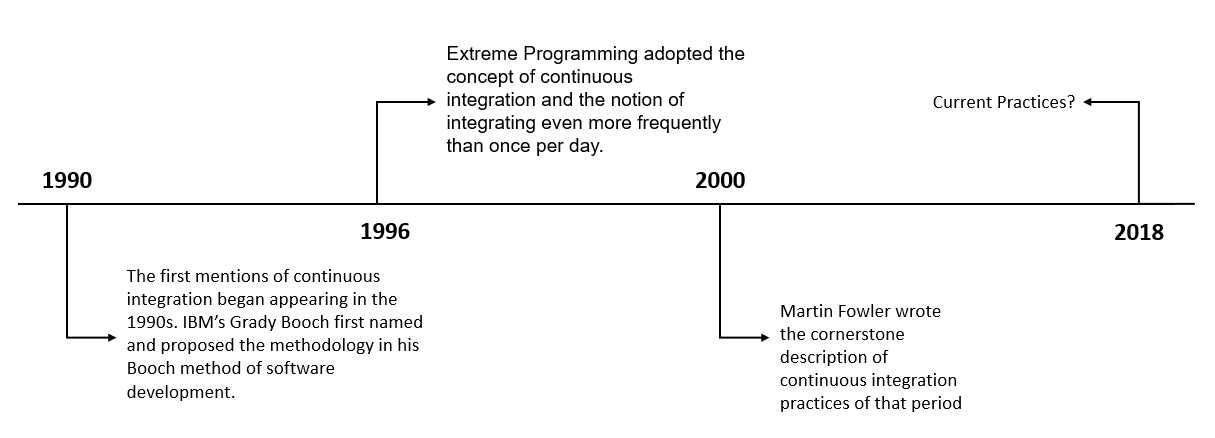
\includegraphics{figures/build-analytics/state_pr.png}
\caption{CI overview.}
\end{figure}

The papers identified using the research protocol defined in section
\ref{build-analytics-research-protocol} that give us an overview of the
current state of the art in build analytics domain are:

\begin{itemize}
\tightlist
\item
  Usage, Costs, and Benefits of Continuous Integration in Open-Source
  Projects {[}\protect\hyperlink{ref-hilton2016usage}{60}{]}
\item
  An Empirical Analysis of Build Failures in the Continuous Integration
  Workflows of Java-Based Open-Source Software
  {[}\protect\hyperlink{ref-rausch2017empirical}{100}{]}
\item
  Continuous Integration
  {[}\protect\hyperlink{ref-fowler2006continuous}{50}{]}
\item
  Enabling Agile Testing Through Continuous Integration
  {[}\protect\hyperlink{ref-stolberg2009enabling}{109}{]}
\item
  Travistorrent: Synthesizing Travis~CI and Github for Full-Stack
  Research on Continuous Integration
  {[}\protect\hyperlink{ref-beller2017travistorrent}{17}{]}
\item
  I'm Leaving You, Travis: A Continuous Integration Breakup Story
  {[}\protect\hyperlink{ref-widder2018m}{119}{]}
\item
  Continuous integration in a social-coding world: Empirical evidence
  from GITHUB {[}\protect\hyperlink{ref-vasilescu2014continuous}{115}{]}
\end{itemize}

The topics that are being explored are:

\begin{itemize}
\tightlist
\item
  Usage of CI in the industry by
  {[}\protect\hyperlink{ref-hilton2016usage}{60}{]}
\item
  Growing popularity of CI due to the introduction of VCS as suggested
  by {[}\protect\hyperlink{ref-rausch2017empirical}{100}{]}
\item
  Common practices used in the industry exemplified by
  {[}\protect\hyperlink{ref-fowler2006continuous}{50}{]}
\item
  Use of common CI practice in the agile approach presented by
  {[}\protect\hyperlink{ref-stolberg2009enabling}{109}{]}
\item
  Comparison between pull requests and direct commits to result in
  successful build as uncovered by
  {[}\protect\hyperlink{ref-vasilescu2014continuous}{115}{]}
\end{itemize}

\subsubsection{Build Analytics Usage}\label{build-analytics-usage}

A survey conducted in open-source projects by Hilton et al.
{[}\protect\hyperlink{ref-hilton2016usage}{60}{]} indicated that 40\% of
all projects used CI. It observed that a median project introduces CI a
year into development. Furthermore, the paper claims that CI is widely
used in practice nowadays. One of many factors contributing to this is
explored by Rausch et al.
{[}\protect\hyperlink{ref-rausch2017empirical}{100}{]}. The growing
popularity of Version Control Systems (VCS) such as GitHub, and hosting
build automation platforms such as Travis have enabled any business of
size to adopt the CI framework. As suggested by Hilton et al.
{[}\protect\hyperlink{ref-hilton2016usage}{60}{]}, the cost and time
associated with introducing the CI framework is not enormous and the
copious benefits far outweigh the resources required.

\subsubsection{Build Analytics
Practices}\label{build-analytics-practices}

The CI concept, often attributed to Martin Fowler
{[}\protect\hyperlink{ref-fowler2006continuous}{50}{]} , is recommended
as best practice of agile software development methods such as extreme
Programming {[}\protect\hyperlink{ref-stolberg2009enabling}{109}{]}. He
introduced many practices that are essential in maintaining the CI
framework. Fowler and Foemmel
{[}\protect\hyperlink{ref-fowler2006continuous}{50}{]} urges engineers
to keep all artifacts required to build the project in a single
repository. This ensures that the system does not require additional
dependencies. In addition, he advises creating a build script that can
compile the code, execute unit tests and automate integration. Once the
code is built, all tests should run to confirm that it behaves as the
developer would expect it to behave. In this way, we are finding and
eradicating software bugs earlier and keeping builds fast. As explored
by Widder et al.{[}\protect\hyperlink{ref-widder2018m}{119}{]}, one of
the factors that lead to companies abandoning the CI framework is the
complexity of the build. A good practice is to have more fast-executing
tests than slow tests.

Furthermore, builds should be readily available to stakeholders and
testers as this can reduce the amount of rework required when rebuilding
a feature that does not meet requirements. In general, all companies
should schedule a ``nightly build'' to update the project from the
repository to ensure everyone is up to date. Continuous Integration is
all about communication, so it is important to ensure that everyone can
easily see the current state of the system. This is also another reason
why CI works well in the agile industry
{[}\protect\hyperlink{ref-stolberg2009enabling}{109}{]}. Both techniques
stress the importance of good communication.

The paper by Vasilescu et al.
{[}\protect\hyperlink{ref-vasilescu2014continuous}{115}{]} studies a
sample of large and active GitHub projects developed in Java, Python and
Ruby. The paper finds that direct code modifications (commits) and more
popular than indirect code modifications (pull request). Additionally,
the notion of automated testing is not as widely practiced. Most samples
in Vasilescu {[}\protect\hyperlink{ref-vasilescu2014continuous}{115}{]}
study were configured to use Travis~CI, however, less than half do. In
terms of languages, Ruby projects are among the early adopters of
Travis~CI, while Java projects are late to adopt CI. The paper uncovers
that the pull requests are much more likely to result in successful
builds than direct commits.

\subsection{Build Analytics Future
Research}\label{build-analytics-future-research}

\textbf{RQ3}: What future research can we expect in the field of build
analytics?

Currently research on build analytics is limited by some challenges,
some are specific to build analytics and some are applicable to the
entire field of software engineering.

The papers identified using the research protocol defined in section
\ref{build-analytics-research-protocol} that give us an overview of
challenges and future research in the field of build analytics are:

\begin{itemize}
\tightlist
\item
  Built to last or built too fast?: evaluating prediction models for
  build times {[}\protect\hyperlink{ref-bisong2017built}{22}{]}
\item
  Work Practices and Challenges in Continuous Integration: A Survey with
  Travis~CI Users {[}\protect\hyperlink{ref-pinto2018work}{93}{]}
\item
  Statically Verifying Continuous Integration Configurations
  {[}\protect\hyperlink{ref-santolucito2018statically}{104}{]}
\item
  (No) Influence of Continuous Integration on the Commit Activity in
  GitHub Projects {[}\protect\hyperlink{ref-baltes2018no}{8}{]}
\item
  The impact of continuous integration on other software development
  practices: a large-scale empirical study
  {[}\protect\hyperlink{ref-zhao2017impact}{124}{]}
\item
  Un-Break My Build: Assisting Developers with Build Repair Hints
  {[}\protect\hyperlink{ref-vassallo2018break}{116}{]}
\item
  Oops, my tests broke the build: An explorative analysis of Travis~CI
  with GitHub {[}\protect\hyperlink{ref-beller2017oops}{16}{]}
\end{itemize}

In Bisong et al.{[}\protect\hyperlink{ref-bisong2017built}{22}{]} the
main limitation was the performance of the machine learning algorithm
used. In the implementation R was used and it proved not capable of
processing the amounts of data needed. This shows that it is important
to choose the right tool when analyzing data.

In Pinto and Rebouças{[}\protect\hyperlink{ref-pinto2018work}{93}{]} it
is noted that research is often done on open source software. There are
still a lot of possibilities for researching on proprietary software
projects.

Tools presented in papers might require a more large-scale and long-term
study to verify that the tool presented keeps up when it is
used{[}\protect\hyperlink{ref-santolucito2018statically}{104}{]}.

Future research in build analytics branches in a couple of different
topics. Pinto and
Rebouças{[}\protect\hyperlink{ref-pinto2018work}{93}{]} proposes to
focus on getting a better understanding of the users and why they might
choose to abandon an automatic build platform.

Baltes et al.{[}\protect\hyperlink{ref-baltes2018no}{8}{]} suggest that
in future research more perspectives when analyzing commit data should
be considered, for instance partitioning commits by developer. It also
notes the importance of more qualitative research.

Some open research questions from recent papers are the following:

\begin{itemize}
\tightlist
\item
  How do teams change their pull request review practices in response to
  the introduction of continuous integration?
  {[}\protect\hyperlink{ref-zhao2017impact}{124}{]}
\item
  How can we detect if fixing a build configuration requires changes in
  the remote environment?
  {[}\protect\hyperlink{ref-vassallo2018break}{116}{]}
\item
  Does breaking the build often translate to worse project quality and
  decreased productivity?
  {[}\protect\hyperlink{ref-beller2017oops}{16}{]}
\item
  Could already trained models on projects with more data available be
  used to make accurate predictions on newer projects with less data
  available? {[}\protect\hyperlink{ref-ni2018acona}{91}{]}
\end{itemize}

From the synthesis of the works discussed in this section the following
research questions emerged:

\begin{itemize}
\tightlist
\item
  What is the impact of the choice of Continuous Integration platform?
  Most of the research is done on users using Travis~CI, there are many
  other platforms out there. Every platform has their own
  characteristics and this could impact the effectiveness for a specific
  kind of project.
\item
  How does the platform or programming language influence effectiveness
  or adoption of continuous integration systems?
\item
  How can machine learning methods be better applied in the field of
  build analytics in order to generate predictions that are easier to
  explain and thus that can be used in practice?
\end{itemize}

\chapter*{Appendix: Build Analytics}\label{appendix-build-analytics}
\addcontentsline{toc}{chapter}{Appendix: Build Analytics}

\begin{longtable}[]{@{}llll@{}}
\caption{\label{tab:build-analytics-selected-papers} Selected
papers}\tabularnewline
\toprule
\begin{minipage}[b]{0.48\columnwidth}\raggedright\strut
Paper with reference\strut
\end{minipage} & \begin{minipage}[b]{0.20\columnwidth}\raggedright\strut
Source\strut
\end{minipage} & \begin{minipage}[b]{0.14\columnwidth}\raggedright\strut
RQ\strut
\end{minipage} & \begin{minipage}[b]{0.06\columnwidth}\raggedright\strut
Notes\strut
\end{minipage}\tabularnewline
\midrule
\endfirsthead
\toprule
\begin{minipage}[b]{0.48\columnwidth}\raggedright\strut
Paper with reference\strut
\end{minipage} & \begin{minipage}[b]{0.20\columnwidth}\raggedright\strut
Source\strut
\end{minipage} & \begin{minipage}[b]{0.14\columnwidth}\raggedright\strut
RQ\strut
\end{minipage} & \begin{minipage}[b]{0.06\columnwidth}\raggedright\strut
Notes\strut
\end{minipage}\tabularnewline
\midrule
\endhead
\begin{minipage}[t]{0.48\columnwidth}\raggedright\strut
1. Bird et al. 2017
{[}\protect\hyperlink{ref-bird2017predicting}{20}{]}\strut
\end{minipage} & \begin{minipage}[t]{0.20\columnwidth}\raggedright\strut
Initial seed\strut
\end{minipage} & \begin{minipage}[t]{0.14\columnwidth}\raggedright\strut
RQ1\strut
\end{minipage} & \begin{minipage}[t]{0.06\columnwidth}\raggedright\strut
1\strut
\end{minipage}\tabularnewline
\begin{minipage}[t]{0.48\columnwidth}\raggedright\strut
2. Beller et al. 2017
{[}\protect\hyperlink{ref-beller2017oops}{16}{]}\strut
\end{minipage} & \begin{minipage}[t]{0.20\columnwidth}\raggedright\strut
Initial seed\strut
\end{minipage} & \begin{minipage}[t]{0.14\columnwidth}\raggedright\strut
RQ3\strut
\end{minipage} & \begin{minipage}[t]{0.06\columnwidth}\raggedright\strut
-\strut
\end{minipage}\tabularnewline
\begin{minipage}[t]{0.48\columnwidth}\raggedright\strut
3. Rausch et al. 2017
{[}\protect\hyperlink{ref-rausch2017empirical}{100}{]}\strut
\end{minipage} & \begin{minipage}[t]{0.20\columnwidth}\raggedright\strut
Initial seed\strut
\end{minipage} & \begin{minipage}[t]{0.14\columnwidth}\raggedright\strut
RQ2\strut
\end{minipage} & \begin{minipage}[t]{0.06\columnwidth}\raggedright\strut
-\strut
\end{minipage}\tabularnewline
\begin{minipage}[t]{0.48\columnwidth}\raggedright\strut
4. Beller et al. TravisTorrent 2017
{[}\protect\hyperlink{ref-beller2017travistorrent}{17}{]}\strut
\end{minipage} & \begin{minipage}[t]{0.20\columnwidth}\raggedright\strut
Initial seed\strut
\end{minipage} & \begin{minipage}[t]{0.14\columnwidth}\raggedright\strut
RQ2\strut
\end{minipage} & \begin{minipage}[t]{0.06\columnwidth}\raggedright\strut
-\strut
\end{minipage}\tabularnewline
\begin{minipage}[t]{0.48\columnwidth}\raggedright\strut
5. Pinto et al. 2018
{[}\protect\hyperlink{ref-pinto2018work}{93}{]}\strut
\end{minipage} & \begin{minipage}[t]{0.20\columnwidth}\raggedright\strut
Initial seed\strut
\end{minipage} & \begin{minipage}[t]{0.14\columnwidth}\raggedright\strut
RQ3\strut
\end{minipage} & \begin{minipage}[t]{0.06\columnwidth}\raggedright\strut
-\strut
\end{minipage}\tabularnewline
\begin{minipage}[t]{0.48\columnwidth}\raggedright\strut
6. Zhao et al. 2017
{[}\protect\hyperlink{ref-zhao2017impact}{124}{]}\strut
\end{minipage} & \begin{minipage}[t]{0.20\columnwidth}\raggedright\strut
Initial seed\strut
\end{minipage} & \begin{minipage}[t]{0.14\columnwidth}\raggedright\strut
RQ3\strut
\end{minipage} & \begin{minipage}[t]{0.06\columnwidth}\raggedright\strut
2\strut
\end{minipage}\tabularnewline
\begin{minipage}[t]{0.48\columnwidth}\raggedright\strut
7. Widder et al. 2018
{[}\protect\hyperlink{ref-widder2018m}{119}{]}\strut
\end{minipage} & \begin{minipage}[t]{0.20\columnwidth}\raggedright\strut
Initial seed\strut
\end{minipage} & \begin{minipage}[t]{0.14\columnwidth}\raggedright\strut
RQ1\strut
\end{minipage} & \begin{minipage}[t]{0.06\columnwidth}\raggedright\strut
-\strut
\end{minipage}\tabularnewline
\begin{minipage}[t]{0.48\columnwidth}\raggedright\strut
8. Hilton et al. 2016
{[}\protect\hyperlink{ref-hilton2016usage}{60}{]}\strut
\end{minipage} & \begin{minipage}[t]{0.20\columnwidth}\raggedright\strut
Initial seed\strut
\end{minipage} & \begin{minipage}[t]{0.14\columnwidth}\raggedright\strut
RQ2\strut
\end{minipage} & \begin{minipage}[t]{0.06\columnwidth}\raggedright\strut
-\strut
\end{minipage}\tabularnewline
\begin{minipage}[t]{0.48\columnwidth}\raggedright\strut
9. Vassallo et al. 2017
{[}\protect\hyperlink{ref-vassallo2017tale}{117}{]}\strut
\end{minipage} & \begin{minipage}[t]{0.20\columnwidth}\raggedright\strut
Ref 2\strut
\end{minipage} & \begin{minipage}[t]{0.14\columnwidth}\raggedright\strut
-\strut
\end{minipage} & \begin{minipage}[t]{0.06\columnwidth}\raggedright\strut
3\strut
\end{minipage}\tabularnewline
\begin{minipage}[t]{0.48\columnwidth}\raggedright\strut
11. Hassan and Wang 2018
{[}\protect\hyperlink{ref-hassan2018hirebuild}{57}{]}\strut
\end{minipage} & \begin{minipage}[t]{0.20\columnwidth}\raggedright\strut
Ref 4\strut
\end{minipage} & \begin{minipage}[t]{0.14\columnwidth}\raggedright\strut
RQ1\strut
\end{minipage} & \begin{minipage}[t]{0.06\columnwidth}\raggedright\strut
-\strut
\end{minipage}\tabularnewline
\begin{minipage}[t]{0.48\columnwidth}\raggedright\strut
12. Vassallo et al. 2018
{[}\protect\hyperlink{ref-vassallo2018break}{116}{]}\strut
\end{minipage} & \begin{minipage}[t]{0.20\columnwidth}\raggedright\strut
Ref 2,3\strut
\end{minipage} & \begin{minipage}[t]{0.14\columnwidth}\raggedright\strut
RQ1, RQ3\strut
\end{minipage} & \begin{minipage}[t]{0.06\columnwidth}\raggedright\strut
-\strut
\end{minipage}\tabularnewline
\begin{minipage}[t]{0.48\columnwidth}\raggedright\strut
13. Zampetti et al. 2017
{[}\protect\hyperlink{ref-zampetti2017open}{122}{]}\strut
\end{minipage} & \begin{minipage}[t]{0.20\columnwidth}\raggedright\strut
Ref by 12\strut
\end{minipage} & \begin{minipage}[t]{0.14\columnwidth}\raggedright\strut
-\strut
\end{minipage} & \begin{minipage}[t]{0.06\columnwidth}\raggedright\strut
3\strut
\end{minipage}\tabularnewline
\begin{minipage}[t]{0.48\columnwidth}\raggedright\strut
14. Baltes et al. 2018
{[}\protect\hyperlink{ref-baltes2018no}{8}{]}\strut
\end{minipage} & \begin{minipage}[t]{0.20\columnwidth}\raggedright\strut
GScholar Search\strut
\end{minipage} & \begin{minipage}[t]{0.14\columnwidth}\raggedright\strut
RQ1, RQ3\strut
\end{minipage} & \begin{minipage}[t]{0.06\columnwidth}\raggedright\strut
4\strut
\end{minipage}\tabularnewline
\begin{minipage}[t]{0.48\columnwidth}\raggedright\strut
15. Bisong et al. 2017
{[}\protect\hyperlink{ref-bisong2017built}{22}{]}\strut
\end{minipage} & \begin{minipage}[t]{0.20\columnwidth}\raggedright\strut
GScholar Search\strut
\end{minipage} & \begin{minipage}[t]{0.14\columnwidth}\raggedright\strut
RQ1, RQ3\strut
\end{minipage} & \begin{minipage}[t]{0.06\columnwidth}\raggedright\strut
5\strut
\end{minipage}\tabularnewline
\begin{minipage}[t]{0.48\columnwidth}\raggedright\strut
16. Santolucito et al. 2018
{[}\protect\hyperlink{ref-santolucito2018statically}{104}{]}\strut
\end{minipage} & \begin{minipage}[t]{0.20\columnwidth}\raggedright\strut
GScholar Search\strut
\end{minipage} & \begin{minipage}[t]{0.14\columnwidth}\raggedright\strut
RQ1\strut
\end{minipage} & \begin{minipage}[t]{0.06\columnwidth}\raggedright\strut
4\strut
\end{minipage}\tabularnewline
\begin{minipage}[t]{0.48\columnwidth}\raggedright\strut
17. Ni and Li 2018 {[}\protect\hyperlink{ref-ni2018acona}{91}{]}\strut
\end{minipage} & \begin{minipage}[t]{0.20\columnwidth}\raggedright\strut
GScholar Search\strut
\end{minipage} & \begin{minipage}[t]{0.14\columnwidth}\raggedright\strut
RQ1\strut
\end{minipage} & \begin{minipage}[t]{0.06\columnwidth}\raggedright\strut
6\strut
\end{minipage}\tabularnewline
\begin{minipage}[t]{0.48\columnwidth}\raggedright\strut
18. Fowler and Foemmel 2006
{[}\protect\hyperlink{ref-fowler2006continuous}{50}{]}\strut
\end{minipage} & \begin{minipage}[t]{0.20\columnwidth}\raggedright\strut
GScholar Search\strut
\end{minipage} & \begin{minipage}[t]{0.14\columnwidth}\raggedright\strut
RQ2\strut
\end{minipage} & \begin{minipage}[t]{0.06\columnwidth}\raggedright\strut
7\strut
\end{minipage}\tabularnewline
\begin{minipage}[t]{0.48\columnwidth}\raggedright\strut
19. Stolberg 2009
{[}\protect\hyperlink{ref-stolberg2009enabling}{109}{]}\strut
\end{minipage} & \begin{minipage}[t]{0.20\columnwidth}\raggedright\strut
GScholar Search\strut
\end{minipage} & \begin{minipage}[t]{0.14\columnwidth}\raggedright\strut
RQ2\strut
\end{minipage} & \begin{minipage}[t]{0.06\columnwidth}\raggedright\strut
7\strut
\end{minipage}\tabularnewline
\begin{minipage}[t]{0.48\columnwidth}\raggedright\strut
20. Vasilescu et al. 2014
{[}\protect\hyperlink{ref-vasilescu2014continuous}{115}{]}\strut
\end{minipage} & \begin{minipage}[t]{0.20\columnwidth}\raggedright\strut
GScholar Search\strut
\end{minipage} & \begin{minipage}[t]{0.14\columnwidth}\raggedright\strut
RQ2\strut
\end{minipage} & \begin{minipage}[t]{0.06\columnwidth}\raggedright\strut
7\strut
\end{minipage}\tabularnewline
\bottomrule
\end{longtable}

\textbf{Notes}

\begin{enumerate}
\def\labelenumi{\arabic{enumi}.}
\tightlist
\item
  US patent owned by Microsoft.
\item
  Collaboration between universities in China, The Netherlands and The
  USA.
\item
  Not included in this survey as it did not introduce a new technique or
  practice.
\item
  Using search term ``Github Continuous Integration''.
\item
  Using search term ``Predicting build time''
\item
  Using search term ``Predicting build failures''
\item
  Using search term ``Current practices in Continuous Integration''
\end{enumerate}

\chapter{Bug Prediction}\label{bug-prediction}

\section{Motivation}\label{motivation-2}

Minimizing the number of bugs in software is an effort central to
software engineering - faulty code fails to fullfill the purpose it was
written for, its impact ranges from sligthly embarrassing to disastrous
and dangerous, and last but not least - fixing it costs time and money.
Resources in a software development lifecycle are almost always limited
and therefore should be allocated to where they are needed most - in
order to avoid bugs, they should be focused on the most fault-prone
areas of the project. Being able to predict where such areas might be
would allow more development and testing efforts to be allocated on the
right places.

However, as noted in {[}\protect\hyperlink{ref-DAmbros2012}{47}{]},
reliably predicting which parts of source code are the most fault-prone
is one of the holy-grails of software engineering. Thus it is not
surprising that bug-prediction continues to garner a widespread research
interest in software analytics, now equipped with the ever-expanding
toolbox of data-mining and machine learning techniques. In this survey
we investigate the current efforts in bug-prediction in the light of the
advances in software analytics methods and focus our attention on
answering the following research questions:

\begin{itemize}
\tightlist
\item
  \textbf{RQ1} What is the current state of the art in bug prediction?
  More specifically, we aim to answer the following:

  \begin{itemize}
  \tightlist
  \item
    What software or other metrics does bug prediction rely on and how
    good are they?
  \item
    What kind prediction models are predominantly used?
  \item
    How are bug prediction models and results validated and evaluated?
  \end{itemize}
\item
  \textbf{RQ2} What is the current state of practice in bug prediction?

  \begin{itemize}
  \tightlist
  \item
    Are bug prediction techniques applied in practice and if so, how?
  \item
    Are the current developments in the field able to provide actionable
    tools for developers?
  \end{itemize}
\item
  \textbf{RQ3} What are some of the open challenges and directions for
  future research?
\end{itemize}

\section{Research protocol}\label{research-protocol-1}

We started by studying the initial 6 seed papers which were selected
based on domain knowledge:

\begin{itemize}
\tightlist
\item
  {[}\protect\hyperlink{ref-Gyimothy2005}{55}{]}
\item
  {[}\protect\hyperlink{ref-Catal2009review}{29}{]}
\item
  {[}\protect\hyperlink{ref-Arisholm2010}{5}{]}
\item
  {[}\protect\hyperlink{ref-DAmbros2010}{46}{]}
\item
  {[}\protect\hyperlink{ref-Hall2012}{56}{]}
\item
  {[}\protect\hyperlink{ref-Lewis2013}{78}{]}
\end{itemize}

Our searches were based on the following elements:

\begin{enumerate}
\def\labelenumi{\arabic{enumi}.}
\item
  Keyword search using search engines (Scopus, ACM Digital Library, IEEE
  Explorer). The search query was constructed so that the paper title
  had to contain the phrase bug prediction, but also the other more
  general variants used in literature: \emph{bug/defect/fault
  prediction}. The title also had to contain at least one of following
  keywords: \emph{metrics}, \emph{models}, \emph{validation},
  \emph{evaluation}, \emph{developers}. To remain within the bug
  prediction field we required \emph{software} to appear in the
  abstract.
\item
  Filtering search results by publication date. We excluded papers older
  than 10 years; that is, published before 2008.
\item
  Filtering by the number of citations. We selected papers with 10 or
  more citations in order to focus on the ones that already have some
  visibility within the field.
\item
  Exploring other impactful publications by the same authors.
\end{enumerate}

\emph{Table 1. Papers found by investigating the authors of other
papers.}

\begin{longtable}[]{@{}lll@{}}
\toprule
Starting point & Type & Result\tabularnewline
\midrule
\endhead
{[}\protect\hyperlink{ref-DAmbros2010}{46}{]} & is author of &
{[}\protect\hyperlink{ref-DAmbros2012}{47}{]}\tabularnewline
{[}\protect\hyperlink{ref-Catal2009review}{29}{]} & is author of &
{[}\protect\hyperlink{ref-Catal2011}{28}{]}
{[}\protect\hyperlink{ref-Catal2009investigating}{30}{]}\tabularnewline
\bottomrule
\end{longtable}

\section{Answers}\label{answers-1}

\chapter{Ecosystem Analytics}\label{ecosystem-analytics}

\section{Motivation}\label{motivation-3}

In the modern day and age, the majority of software products make use of
external software or libraries to use the functionality (for example
parsing JSON) of these products, without having to develop this
functionality itself. Moreover, multiple languages, such as Python and
Rust, provide package managers (pip\footnote{\url{https://pypi.org/project/pip/}}
and Cargo\footnote{\url{https://crates.io/}} respectively) which can be
used to easily manage this third-party functionality, as well as
distribute it.

In parallel to this, the popularity of creating open source projects is
on the rise as well. On platforms such as GitHub\footnote{\url{https://github.com:}},
it is easy and quick to create a new software project, which can be
developed, reviewed and used by the whole community. This development
leads to more libraries being developed and being available for public
use.

Because of these two developments, further inspection of the dependency
relations between projects leads to a graph-like structure of software
projects, where the nodes are the projects and the edges represent a
dependency between two software projects. This structure is known as a
\emph{software ecosystem}. As stated by
{[}\protect\hyperlink{ref-Messerschmitt2003}{88}{]}, a \emph{software
ecosystem} is ``a collection of software products that have some given
degree of symbiotic relationships.'' Another, similar definition is
given by {[}\protect\hyperlink{ref-Lungu2009}{79}{]}: ``A software
ecosystem is a collection of software projects which are developed and
co-evolve in the same environment.''
{[}\protect\hyperlink{ref-Mens2013}{87}{]} extends this definition, ``by
explicitly considering the communities involved (e.g.~user and developer
communities) as being part of the software ecosystem.''
{[}\protect\hyperlink{ref-Stallman2002}{108}{]} opposes the overall
notion of calling this structure a software ecosystem: ``It is
inadvisable to describe the free software community, or any human
community, as an ecosystem, because that word implies the absence of
ethical judgment.''

Although {[}\protect\hyperlink{ref-Stallman2002}{108}{]} thinks that the
term software ecosystem itself is incorrect, it does not necessarily
disagree with the definition of the term. The definition which will be
used in this chapter is the definition of
{[}\protect\hyperlink{ref-Mens2013}{87}{]}, since it captures the
essence of the other two definitions, while adding the notion of the
human communities alongside as well.

By performing analysis on these software ecosystems, the aim is to
generate meaningful insights. These insights can then be used to improve
the efficiency and effectivity of the software development process, as
well as to learn to identify and inform about potential problems. For
example, a warning could be displayed if a dependency has a security
vulnerability.

The field of research on software ecosystems, \emph{ecosystem
analytics}, focuses on performing such analysis. This chapter discovers
what the current progress is in this field of research through a
literature survey. This discovery is not limited to the theoretical
perspective, but will uncover practical implications as well as the open
challenges of the field. In order to describe each covered aspect, we
have formulated three research questions:

\begin{itemize}
\tightlist
\item
  \textbf{RQ1}: What is the current state of the art in software
  analytics for ecosystem analytics?
\item
  \textbf{RQ2}: What are the practical implications from the state of
  the art?
\item
  \textbf{RQ3}: What are the open challenges in ecosystem analytics, for
  which future research is required?
\end{itemize}

Each of these research questions will be answered using recent papers
written in this field of research.

This chapter is structured as follows. First, the research protocol is
described in detail. This includes decisions on which papers are
included in the review. After this, the research questions are answered
using the previously stated set of papers.

\section{Research Protocol}\label{research-protocol-2}

In order to select literature to answer the research questions given in
the previous section, the survey method suggested by
{[}\protect\hyperlink{ref-Kitchenham2004}{72}{]} is used. This method
creates a systematic way to select a set of papers, which is relevant to
the research question(s).

The search strategy, as described by
{[}\protect\hyperlink{ref-Kitchenham2004}{72}{]}, are usually iterative
and benefit from consultations with experts in the field, amongst other
things. Our search strategy can be split in three different types:

\begin{itemize}
\tightlist
\item
  the initial seed, given by an expert in the field, MSc. Joseph
  Hejderup
\item
  a search using a digital search engine, namely Google
  Scholar\footnote{\url{https://github.com:}}
\item
  a selection of referenced papers within papers selected before in the
  above two searches
\end{itemize}

In order to select literature to answer the research questions given in
the previous section, the survey method suggested by
{[}\protect\hyperlink{ref-Kitchenham2004}{72}{]} is used. This method
creates a systematic way to select a set of papers, which is relevant to
the research question(s).

The search strategy, as described by
{[}\protect\hyperlink{ref-Kitchenham2004}{72}{]}, are usually iterative
and benefit from consultations with experts in the field, amongst other
things. Our search strategy can be split in three different types:

\begin{itemize}
\tightlist
\item
  the initial seed, given by an expert in the field, MSc. Joseph
  Hejderup
\item
  a search using a digital search engine, namely Google
  Scholar\footnote{\url{https://github.com:}}
\item
  a selection of referenced papers within papers selected before in the
  above two searches
\end{itemize}

\subsection{Initial seed}\label{initial-seed}

MSc. Joseph Hejderup has provided us with a total of thirteen papers, as
shown in Table 1.

As each of these papers come from an expert in the field, each paper is
assumed to be relevant to atleast the field of software ecosystems.
Because of this, each of these papers were judged on their relevance to
either of the research questions. In Table 1, this relevance judgment is
shown in the left column, since a paper is only selected, if the paper
is indeed relevant. Table 2 describes the reason for which each
particular paper is not selected for the literature survey.

\begin{longtable}[]{@{}lllll@{}}
\toprule
\begin{minipage}[b]{0.01\columnwidth}\raggedright\strut
Selected\strut
\end{minipage} & \begin{minipage}[b]{0.09\columnwidth}\raggedright\strut
Author(s)\strut
\end{minipage} & \begin{minipage}[b]{0.34\columnwidth}\raggedright\strut
Title\strut
\end{minipage} & \begin{minipage}[b]{0.02\columnwidth}\raggedright\strut
Year\strut
\end{minipage} & \begin{minipage}[b]{0.39\columnwidth}\raggedright\strut
Keywords\strut
\end{minipage}\tabularnewline
\midrule
\endhead
\begin{minipage}[t]{0.01\columnwidth}\raggedright\strut
-\strut
\end{minipage} & \begin{minipage}[t]{0.09\columnwidth}\raggedright\strut
{[}\protect\hyperlink{ref-Abate2009}{2}{]}\strut
\end{minipage} & \begin{minipage}[t]{0.34\columnwidth}\raggedright\strut
Strong dependencies between software components\strut
\end{minipage} & \begin{minipage}[t]{0.02\columnwidth}\raggedright\strut
2009\strut
\end{minipage} & \begin{minipage}[t]{0.39\columnwidth}\raggedright\strut
\strut
\end{minipage}\tabularnewline
\begin{minipage}[t]{0.01\columnwidth}\raggedright\strut
-\strut
\end{minipage} & \begin{minipage}[t]{0.09\columnwidth}\raggedright\strut
{[}\protect\hyperlink{ref-Abate2011}{1}{]}\strut
\end{minipage} & \begin{minipage}[t]{0.34\columnwidth}\raggedright\strut
Predicting upgrade failures using dependency analysis\strut
\end{minipage} & \begin{minipage}[t]{0.02\columnwidth}\raggedright\strut
2011\strut
\end{minipage} & \begin{minipage}[t]{0.39\columnwidth}\raggedright\strut
\strut
\end{minipage}\tabularnewline
\begin{minipage}[t]{0.01\columnwidth}\raggedright\strut
+\strut
\end{minipage} & \begin{minipage}[t]{0.09\columnwidth}\raggedright\strut
{[}\protect\hyperlink{ref-Abdalkareem2017}{3}{]}\strut
\end{minipage} & \begin{minipage}[t]{0.34\columnwidth}\raggedright\strut
Why do developers use trivial packages? An empirical case study on
NPM\strut
\end{minipage} & \begin{minipage}[t]{0.02\columnwidth}\raggedright\strut
2017\strut
\end{minipage} & \begin{minipage}[t]{0.39\columnwidth}\raggedright\strut
JavaScript; Node.js; Code Reuse; Empirical Studies\strut
\end{minipage}\tabularnewline
\begin{minipage}[t]{0.01\columnwidth}\raggedright\strut
+\strut
\end{minipage} & \begin{minipage}[t]{0.09\columnwidth}\raggedright\strut
{[}\protect\hyperlink{ref-Bogart2016}{24}{]}\strut
\end{minipage} & \begin{minipage}[t]{0.34\columnwidth}\raggedright\strut
How to break an api: Cost negotiation and community values in three
software ecosystem\strut
\end{minipage} & \begin{minipage}[t]{0.02\columnwidth}\raggedright\strut
2016\strut
\end{minipage} & \begin{minipage}[t]{0.39\columnwidth}\raggedright\strut
Software ecosystems; Dependency management; semantic versioning;
Collaboration; Qualitative research\strut
\end{minipage}\tabularnewline
\begin{minipage}[t]{0.01\columnwidth}\raggedright\strut
+\strut
\end{minipage} & \begin{minipage}[t]{0.09\columnwidth}\raggedright\strut
{[}\protect\hyperlink{ref-Claes2015}{34}{]}\strut
\end{minipage} & \begin{minipage}[t]{0.34\columnwidth}\raggedright\strut
A historical analysis of Debian package incompatibilities\strut
\end{minipage} & \begin{minipage}[t]{0.02\columnwidth}\raggedright\strut
2015\strut
\end{minipage} & \begin{minipage}[t]{0.39\columnwidth}\raggedright\strut
debian, conflict, empirical, analysis, software, evolution,
distribution, package, dependency, maintenance\strut
\end{minipage}\tabularnewline
\begin{minipage}[t]{0.01\columnwidth}\raggedright\strut
+\strut
\end{minipage} & \begin{minipage}[t]{0.09\columnwidth}\raggedright\strut
{[}\protect\hyperlink{ref-Constantinou2017}{35}{]}\strut
\end{minipage} & \begin{minipage}[t]{0.34\columnwidth}\raggedright\strut
An empirical comparison of developer retention in the RubyGems and NPM
software ecosystems\strut
\end{minipage} & \begin{minipage}[t]{0.02\columnwidth}\raggedright\strut
2017\strut
\end{minipage} & \begin{minipage}[t]{0.39\columnwidth}\raggedright\strut
Software ecosystem, Socio-technical interaction, Software evolution,
Empirical analysis, Survival analysis\strut
\end{minipage}\tabularnewline
\begin{minipage}[t]{0.01\columnwidth}\raggedright\strut
+\strut
\end{minipage} & \begin{minipage}[t]{0.09\columnwidth}\raggedright\strut
{[}\protect\hyperlink{ref-Hejderup2018}{58}{]}\strut
\end{minipage} & \begin{minipage}[t]{0.34\columnwidth}\raggedright\strut
Software Ecosystem Call Graph for Dependency Management\strut
\end{minipage} & \begin{minipage}[t]{0.02\columnwidth}\raggedright\strut
2018\strut
\end{minipage} & \begin{minipage}[t]{0.39\columnwidth}\raggedright\strut
\strut
\end{minipage}\tabularnewline
\begin{minipage}[t]{0.01\columnwidth}\raggedright\strut
+\strut
\end{minipage} & \begin{minipage}[t]{0.09\columnwidth}\raggedright\strut
{[}\protect\hyperlink{ref-Kikas2017}{70}{]}\strut
\end{minipage} & \begin{minipage}[t]{0.34\columnwidth}\raggedright\strut
Structure and evolution of package dependency networks\strut
\end{minipage} & \begin{minipage}[t]{0.02\columnwidth}\raggedright\strut
2017\strut
\end{minipage} & \begin{minipage}[t]{0.39\columnwidth}\raggedright\strut
\strut
\end{minipage}\tabularnewline
\begin{minipage}[t]{0.01\columnwidth}\raggedright\strut
+\strut
\end{minipage} & \begin{minipage}[t]{0.09\columnwidth}\raggedright\strut
{[}\protect\hyperlink{ref-Kula2017}{75}{]}\strut
\end{minipage} & \begin{minipage}[t]{0.34\columnwidth}\raggedright\strut
Do developers update their library dependencies?\strut
\end{minipage} & \begin{minipage}[t]{0.02\columnwidth}\raggedright\strut
2017\strut
\end{minipage} & \begin{minipage}[t]{0.39\columnwidth}\raggedright\strut
Software reuse, Software maintenance, Security vulnerabilities\strut
\end{minipage}\tabularnewline
\begin{minipage}[t]{0.01\columnwidth}\raggedright\strut
-\strut
\end{minipage} & \begin{minipage}[t]{0.09\columnwidth}\raggedright\strut
{[}\protect\hyperlink{ref-Mens2013}{87}{]}\strut
\end{minipage} & \begin{minipage}[t]{0.34\columnwidth}\raggedright\strut
Studying Evolving Software Ecosystems based on Ecological Models\strut
\end{minipage} & \begin{minipage}[t]{0.02\columnwidth}\raggedright\strut
2013\strut
\end{minipage} & \begin{minipage}[t]{0.39\columnwidth}\raggedright\strut
Coral Reef, Natural Ecosystem, Open Source Software, Ecological Model,
Software Project\strut
\end{minipage}\tabularnewline
\begin{minipage}[t]{0.01\columnwidth}\raggedright\strut
+\strut
\end{minipage} & \begin{minipage}[t]{0.09\columnwidth}\raggedright\strut
{[}\protect\hyperlink{ref-Raemaekers2017}{98}{]}\strut
\end{minipage} & \begin{minipage}[t]{0.34\columnwidth}\raggedright\strut
Semantic versioning and impact of breaking changes in the Maven
repository\strut
\end{minipage} & \begin{minipage}[t]{0.02\columnwidth}\raggedright\strut
2017\strut
\end{minipage} & \begin{minipage}[t]{0.39\columnwidth}\raggedright\strut
Semantic versioning, Breaking changes, Software libraries\strut
\end{minipage}\tabularnewline
\begin{minipage}[t]{0.01\columnwidth}\raggedright\strut
+\strut
\end{minipage} & \begin{minipage}[t]{0.09\columnwidth}\raggedright\strut
{[}\protect\hyperlink{ref-Robbes2012}{101}{]}\strut
\end{minipage} & \begin{minipage}[t]{0.34\columnwidth}\raggedright\strut
How do developers react to API deprecation? The case of a smalltalk
ecosystem\strut
\end{minipage} & \begin{minipage}[t]{0.02\columnwidth}\raggedright\strut
2012\strut
\end{minipage} & \begin{minipage}[t]{0.39\columnwidth}\raggedright\strut
Ecosystems, Mining Software Repositories, Empirical Studies\strut
\end{minipage}\tabularnewline
\begin{minipage}[t]{0.01\columnwidth}\raggedright\strut
+\strut
\end{minipage} & \begin{minipage}[t]{0.09\columnwidth}\raggedright\strut
{[}\protect\hyperlink{ref-Trockman2018}{114}{]}\strut
\end{minipage} & \begin{minipage}[t]{0.34\columnwidth}\raggedright\strut
Adding sparkle to social coding: An empirical study of repository badges
in the npm ecosystem\strut
\end{minipage} & \begin{minipage}[t]{0.02\columnwidth}\raggedright\strut
2018\strut
\end{minipage} & \begin{minipage}[t]{0.39\columnwidth}\raggedright\strut
\strut
\end{minipage}\tabularnewline
\bottomrule
\end{longtable}

\emph{Table: 1. Papers provided by MSc. Joseph Hejderup. The first
column describes whether the paper of the row will be used. A `+' means
it will be used, a `-' means it will not.}

\begin{longtable}[]{@{}ll@{}}
\toprule
\begin{minipage}[b]{0.05\columnwidth}\raggedright\strut
Paper Reference\strut
\end{minipage} & \begin{minipage}[b]{0.05\columnwidth}\raggedright\strut
Reason not selected\strut
\end{minipage}\tabularnewline
\midrule
\endhead
\begin{minipage}[t]{0.05\columnwidth}\raggedright\strut
{[}\protect\hyperlink{ref-Abate2009}{2}{]}\strut
\end{minipage} & \begin{minipage}[t]{0.05\columnwidth}\raggedright\strut
This paper seems to delve more into one software project itself whereas
we are more interested in the relationship between different software
projects\strut
\end{minipage}\tabularnewline
\begin{minipage}[t]{0.05\columnwidth}\raggedright\strut
{[}\protect\hyperlink{ref-Abate2011}{1}{]}\strut
\end{minipage} & \begin{minipage}[t]{0.05\columnwidth}\raggedright\strut
Similarly to {[}\protect\hyperlink{ref-Abate2009}{2}{]}, we are more
interested in the relationship between different software projects\strut
\end{minipage}\tabularnewline
\begin{minipage}[t]{0.05\columnwidth}\raggedright\strut
{[}\protect\hyperlink{ref-Mens2013}{87}{]}\strut
\end{minipage} & \begin{minipage}[t]{0.05\columnwidth}\raggedright\strut
We were in doubt over this one, it could be useful but we weren't
convinced that it was. Since we already had a lot of material we decided
to not use this\strut
\end{minipage}\tabularnewline
\bottomrule
\end{longtable}

\emph{Table: 2. Papers from the initial seed that were not selected for
the literature survey, along with a specification of the reason why this
is the case.}

\subsection{Digital Search Engine}\label{digital-search-engine}

The second strategy type which is used to select relevant papers for
this literature study, is by a digital search engine. In this literature
survey, Google Scholar\footnote{\url{https://github.com:}} is used. From
the initial seed, common keywords were retrieved and the following
queries have been used to search for relevant papers:

\begin{itemize}
\tightlist
\item
  ``software ecosystems'' AND ``empirical analysis'' \emph{(2018)}
\item
  ``engineering software ecosystems'' \emph{(2014)}
\item
  ``software ecosystem'' AND ``empirical'' \emph{(2014)}
\item
  ``software ecosystem analytics'' \emph{(2014)}
\item
  ``software ecosystem'' AND ``analysis'' \emph{(2017)}
\item
  ``software ecosystem'' AND ``empirical'' \emph{(2018)}
\end{itemize}

For each of these queries, the results were first filtered by the
publish year. These are described by the italic year after each query
above. The papers that are filtered are published earlier than the set
publish year. These specific years were chosen since the survey focuses
on the state of the art within the ecosystem analytics.

After this filtering, we first determined whether a paper was relevant
to the literature survey by examining the title. If it was unclear
whether the paper was indeed relevant by only looking at the title, the
abstract of the paper was examined closely. On these two criteria, each
of the selected papers were judged and ultimately selected. The selected
paper using these method can be found in Table 3.

\begin{longtable}[]{@{}lllll@{}}
\toprule
\begin{minipage}[b]{0.05\columnwidth}\raggedright\strut
First Author\strut
\end{minipage} & \begin{minipage}[b]{0.31\columnwidth}\raggedright\strut
Title\strut
\end{minipage} & \begin{minipage}[b]{0.02\columnwidth}\raggedright\strut
Year\strut
\end{minipage} & \begin{minipage}[b]{0.34\columnwidth}\raggedright\strut
Keywords\strut
\end{minipage} & \begin{minipage}[b]{0.13\columnwidth}\raggedright\strut
Query Used\strut
\end{minipage}\tabularnewline
\midrule
\endhead
\begin{minipage}[t]{0.05\columnwidth}\raggedright\strut
{[}\protect\hyperlink{ref-Decan2018}{41}{]}\strut
\end{minipage} & \begin{minipage}[t]{0.31\columnwidth}\raggedright\strut
An empirical comparison of dependency network evolution in seven
software packaging ecosystems\strut
\end{minipage} & \begin{minipage}[t]{0.02\columnwidth}\raggedright\strut
2018\strut
\end{minipage} & \begin{minipage}[t]{0.34\columnwidth}\raggedright\strut
Software repository mining, Software ecosystem, Package manager,
Dependency network, Software evolution\strut
\end{minipage} & \begin{minipage}[t]{0.13\columnwidth}\raggedright\strut
``software ecosystems'' AND ``empirical analysis''\strut
\end{minipage}\tabularnewline
\begin{minipage}[t]{0.05\columnwidth}\raggedright\strut
{[}\protect\hyperlink{ref-Dittrich2014}{43}{]}\strut
\end{minipage} & \begin{minipage}[t]{0.31\columnwidth}\raggedright\strut
Software engineering beyond the project -- Sustaining software
ecosystems\strut
\end{minipage} & \begin{minipage}[t]{0.02\columnwidth}\raggedright\strut
2014\strut
\end{minipage} & \begin{minipage}[t]{0.34\columnwidth}\raggedright\strut
\strut
\end{minipage} & \begin{minipage}[t]{0.13\columnwidth}\raggedright\strut
engineering software ecosystems\strut
\end{minipage}\tabularnewline
\begin{minipage}[t]{0.05\columnwidth}\raggedright\strut
{[}\protect\hyperlink{ref-Hora2016}{61}{]}\strut
\end{minipage} & \begin{minipage}[t]{0.31\columnwidth}\raggedright\strut
How do developers react to API evolution? A large-scale empirical
study\strut
\end{minipage} & \begin{minipage}[t]{0.02\columnwidth}\raggedright\strut
2016\strut
\end{minipage} & \begin{minipage}[t]{0.34\columnwidth}\raggedright\strut
API evolution, API deprecation, Software ecosystem, Empirical
study\strut
\end{minipage} & \begin{minipage}[t]{0.13\columnwidth}\raggedright\strut
``software ecosystem'' AND ``empirical''\strut
\end{minipage}\tabularnewline
\begin{minipage}[t]{0.05\columnwidth}\raggedright\strut
{[}\protect\hyperlink{ref-Izquierdo2018}{63}{]}\strut
\end{minipage} & \begin{minipage}[t]{0.31\columnwidth}\raggedright\strut
Software Development Analytics for Xen: Why and How\strut
\end{minipage} & \begin{minipage}[t]{0.02\columnwidth}\raggedright\strut
2018\strut
\end{minipage} & \begin{minipage}[t]{0.34\columnwidth}\raggedright\strut
Companies, Ecosystems, Software, Measurement, Object recognition,
Monitoring, Virtualization\strut
\end{minipage} & \begin{minipage}[t]{0.13\columnwidth}\raggedright\strut
software ecosystem analytics\strut
\end{minipage}\tabularnewline
\begin{minipage}[t]{0.05\columnwidth}\raggedright\strut
{[}\protect\hyperlink{ref-Jansen2014}{64}{]}\strut
\end{minipage} & \begin{minipage}[t]{0.31\columnwidth}\raggedright\strut
Measuring the Health of Open Source Software Ecosystems: Beyond the
Scope of Project Health\strut
\end{minipage} & \begin{minipage}[t]{0.02\columnwidth}\raggedright\strut
2014\strut
\end{minipage} & \begin{minipage}[t]{0.34\columnwidth}\raggedright\strut
\strut
\end{minipage} & \begin{minipage}[t]{0.13\columnwidth}\raggedright\strut
``open source software ecosystems''\strut
\end{minipage}\tabularnewline
\begin{minipage}[t]{0.05\columnwidth}\raggedright\strut
{[}\protect\hyperlink{ref-Kula2017-2}{74}{]}\strut
\end{minipage} & \begin{minipage}[t]{0.31\columnwidth}\raggedright\strut
An exploratory study on library aging by monitoring client usage in a
software ecosystem\strut
\end{minipage} & \begin{minipage}[t]{0.02\columnwidth}\raggedright\strut
2017\strut
\end{minipage} & \begin{minipage}[t]{0.34\columnwidth}\raggedright\strut
\strut
\end{minipage} & \begin{minipage}[t]{0.13\columnwidth}\raggedright\strut
``software ecosystem'' AND ``analysis''\strut
\end{minipage}\tabularnewline
\begin{minipage}[t]{0.05\columnwidth}\raggedright\strut
{[}\protect\hyperlink{ref-Malloy2018}{80}{]}\strut
\end{minipage} & \begin{minipage}[t]{0.31\columnwidth}\raggedright\strut
An empirical analysis of the transition from Python 2 to Python 3\strut
\end{minipage} & \begin{minipage}[t]{0.02\columnwidth}\raggedright\strut
2018\strut
\end{minipage} & \begin{minipage}[t]{0.34\columnwidth}\raggedright\strut
Python programming, Programming language evolution, Compliance\strut
\end{minipage} & \begin{minipage}[t]{0.13\columnwidth}\raggedright\strut
``software ecosystem'' AND ``empirical''\strut
\end{minipage}\tabularnewline
\begin{minipage}[t]{0.05\columnwidth}\raggedright\strut
{[}\protect\hyperlink{ref-Manikas2016}{82}{]}\strut
\end{minipage} & \begin{minipage}[t]{0.31\columnwidth}\raggedright\strut
Revisiting software ecosystems Research: A longitudinal literature
study\strut
\end{minipage} & \begin{minipage}[t]{0.02\columnwidth}\raggedright\strut
2016\strut
\end{minipage} & \begin{minipage}[t]{0.34\columnwidth}\raggedright\strut
Software ecosystems; Longitudinal literature study; Software ecosystem
maturity\strut
\end{minipage} & \begin{minipage}[t]{0.13\columnwidth}\raggedright\strut
``Software ecosystems'' OR ``Dependency management'' OR ``semantic
version''\strut
\end{minipage}\tabularnewline
\begin{minipage}[t]{0.05\columnwidth}\raggedright\strut
{[}\protect\hyperlink{ref-Rajlich2014}{99}{]}\strut
\end{minipage} & \begin{minipage}[t]{0.31\columnwidth}\raggedright\strut
Software evolution and maintenance\strut
\end{minipage} & \begin{minipage}[t]{0.02\columnwidth}\raggedright\strut
2014\strut
\end{minipage} & \begin{minipage}[t]{0.34\columnwidth}\raggedright\strut
\strut
\end{minipage} & \begin{minipage}[t]{0.13\columnwidth}\raggedright\strut
Software Evolution and Maintenance\strut
\end{minipage}\tabularnewline
\begin{minipage}[t]{0.05\columnwidth}\raggedright\strut
{[}\protect\hyperlink{ref-Teixeira2015}{111}{]}\strut
\end{minipage} & \begin{minipage}[t]{0.31\columnwidth}\raggedright\strut
Lessons learned from applying social network analysis on an industrial
Free/Libre/Open Source Software Ecosystem\strut
\end{minipage} & \begin{minipage}[t]{0.02\columnwidth}\raggedright\strut
2015\strut
\end{minipage} & \begin{minipage}[t]{0.34\columnwidth}\raggedright\strut
Social network analysis Open source Open-coopetition Software ecosystems
Business models Homophily Cloud computing OpenStack\strut
\end{minipage} & \begin{minipage}[t]{0.13\columnwidth}\raggedright\strut
``software ecosystem analytics''\strut
\end{minipage}\tabularnewline
\bottomrule
\end{longtable}

\emph{Table: 3. Papers selected from searches using Google Scholar. The
column ``Query Used'' describes which of the queries is used to retrieve
the paper.}

\subsection{Referenced papers}\label{referenced-papers}

Finally, a selection of papers has been made by looking at the
references found in papers selected using the two methods above. For
these papers, the selection process is similar to that of the selected
papers using the digital search engine; it is selected when both the
title and the abstract are deemed relevant to the research questions.
This has led to the papers in Table 4. being selected.

\begin{longtable}[]{@{}lllll@{}}
\toprule
\begin{minipage}[b]{0.12\columnwidth}\raggedright\strut
First Author\strut
\end{minipage} & \begin{minipage}[b]{0.31\columnwidth}\raggedright\strut
Title\strut
\end{minipage} & \begin{minipage}[b]{0.02\columnwidth}\raggedright\strut
Year\strut
\end{minipage} & \begin{minipage}[b]{0.24\columnwidth}\raggedright\strut
Keywords\strut
\end{minipage} & \begin{minipage}[b]{0.16\columnwidth}\raggedright\strut
Referenced In\strut
\end{minipage}\tabularnewline
\midrule
\endhead
\begin{minipage}[t]{0.12\columnwidth}\raggedright\strut
{[}\protect\hyperlink{ref-Bavota2014}{11}{]}\strut
\end{minipage} & \begin{minipage}[t]{0.31\columnwidth}\raggedright\strut
How the Apache community upgrades dependencies: an evolutionary
study\strut
\end{minipage} & \begin{minipage}[t]{0.02\columnwidth}\raggedright\strut
2014\strut
\end{minipage} & \begin{minipage}[t]{0.24\columnwidth}\raggedright\strut
Software Ecosystems · Project dependency upgrades · Mining software
repositories\strut
\end{minipage} & \begin{minipage}[t]{0.16\columnwidth}\raggedright\strut
{[}\protect\hyperlink{ref-Kula2017}{75}{]}\strut
\end{minipage}\tabularnewline
\begin{minipage}[t]{0.12\columnwidth}\raggedright\strut
{[}\protect\hyperlink{ref-Blincoe2015}{23}{]}\strut
\end{minipage} & \begin{minipage}[t]{0.31\columnwidth}\raggedright\strut
Ecosystems in GitHub and a method for ecosystem identification using
reference coupling.\strut
\end{minipage} & \begin{minipage}[t]{0.02\columnwidth}\raggedright\strut
2015\strut
\end{minipage} & \begin{minipage}[t]{0.24\columnwidth}\raggedright\strut
\strut
\end{minipage} & \begin{minipage}[t]{0.16\columnwidth}\raggedright\strut
{[}\protect\hyperlink{ref-Constantinou2017}{35}{]}\strut
\end{minipage}\tabularnewline
\begin{minipage}[t]{0.12\columnwidth}\raggedright\strut
{[}\protect\hyperlink{ref-Cox2015}{38}{]}\strut
\end{minipage} & \begin{minipage}[t]{0.31\columnwidth}\raggedright\strut
Measuring Dependency Freshness in Software Systems\strut
\end{minipage} & \begin{minipage}[t]{0.02\columnwidth}\raggedright\strut
2015\strut
\end{minipage} & \begin{minipage}[t]{0.24\columnwidth}\raggedright\strut
\strut
\end{minipage} & \begin{minipage}[t]{0.16\columnwidth}\raggedright\strut
{[}\protect\hyperlink{ref-Kikas2017}{70}{]}\strut
\end{minipage}\tabularnewline
\begin{minipage}[t]{0.12\columnwidth}\raggedright\strut
{[}\protect\hyperlink{ref-Decan2017}{40}{]}\strut
\end{minipage} & \begin{minipage}[t]{0.31\columnwidth}\raggedright\strut
An empirical comparison of dependency issues in OSS packaging
ecosystems\strut
\end{minipage} & \begin{minipage}[t]{0.02\columnwidth}\raggedright\strut
2017\strut
\end{minipage} & \begin{minipage}[t]{0.24\columnwidth}\raggedright\strut
\strut
\end{minipage} & \begin{minipage}[t]{0.16\columnwidth}\raggedright\strut
{[}\protect\hyperlink{ref-Abdalkareem2017}{3}{]},
{[}\protect\hyperlink{ref-Constantinou2017}{35}{]},
{[}\protect\hyperlink{ref-Decan2018}{41}{]}\strut
\end{minipage}\tabularnewline
\begin{minipage}[t]{0.12\columnwidth}\raggedright\strut
{[}\protect\hyperlink{ref-Dietrich2014}{42}{]}\strut
\end{minipage} & \begin{minipage}[t]{0.31\columnwidth}\raggedright\strut
Broken Promises - An Empirical Study into Evolution Problems in Java
Programs Caused by Library Upgrades\strut
\end{minipage} & \begin{minipage}[t]{0.02\columnwidth}\raggedright\strut
2014\strut
\end{minipage} & \begin{minipage}[t]{0.24\columnwidth}\raggedright\strut
\strut
\end{minipage} & \begin{minipage}[t]{0.16\columnwidth}\raggedright\strut
{[}\protect\hyperlink{ref-Raemaekers2017}{98}{]}\strut
\end{minipage}\tabularnewline
\begin{minipage}[t]{0.12\columnwidth}\raggedright\strut
{[}\protect\hyperlink{ref-Malloy2017}{81}{]}\strut
\end{minipage} & \begin{minipage}[t]{0.31\columnwidth}\raggedright\strut
Quantifying the transition from Python 2 to 3: an empirical study of
Python applications.\strut
\end{minipage} & \begin{minipage}[t]{0.02\columnwidth}\raggedright\strut
2017\strut
\end{minipage} & \begin{minipage}[t]{0.24\columnwidth}\raggedright\strut
\strut
\end{minipage} & \begin{minipage}[t]{0.16\columnwidth}\raggedright\strut
{[}\protect\hyperlink{ref-Malloy2018}{80}{]}\strut
\end{minipage}\tabularnewline
\begin{minipage}[t]{0.12\columnwidth}\raggedright\strut
{[}\protect\hyperlink{ref-McDonnell2013}{85}{]}\strut
\end{minipage} & \begin{minipage}[t]{0.31\columnwidth}\raggedright\strut
An empirical study of api stability and adoption in the android
ecosystem\strut
\end{minipage} & \begin{minipage}[t]{0.02\columnwidth}\raggedright\strut
2013\strut
\end{minipage} & \begin{minipage}[t]{0.24\columnwidth}\raggedright\strut
\strut
\end{minipage} & \begin{minipage}[t]{0.16\columnwidth}\raggedright\strut
{[}\protect\hyperlink{ref-Manikas2016}{82}{]}\strut
\end{minipage}\tabularnewline
\bottomrule
\end{longtable}

\emph{Table: 4. Papers selected which are referenced in previously
selected papers. The column ``Referenced In'' describes in which
selected paper the paper is referenced.}

\section{Answers}\label{answers-2}

In this section, an aggregation of information, found in the papers, is
presented. Each subsection of this section focuses on one of the three
research questions posed in Section 1.

\subsection{What is the current state of the art in software analytics
for ecosystem
analytics?}\label{what-is-the-current-state-of-the-art-in-software-analytics-for-ecosystem-analytics}

To answer this research question, we examine the explored topics in
ecosystem analytics. Moreover, we summarize which research methods,
tools and datasets are being used to explore this topics.

The main topic explored in the selected papers are related to the
dependencies within the software ecosystem. One of the main subjects
related to these dependencies is the subject of breaking changes between
different versions of a package.
{[}\protect\hyperlink{ref-Bogart2016}{24}{]} researched the attitude of
developers of Eclipse, CRAN and NPM packages towards making breaking
changes.

\begin{longtable}[]{@{}lllllll@{}}
\toprule
\begin{minipage}[b]{0.09\columnwidth}\raggedright\strut
Reference\strut
\end{minipage} & \begin{minipage}[b]{0.16\columnwidth}\raggedright\strut
Explored topic(s)\strut
\end{minipage} & \begin{minipage}[b]{0.17\columnwidth}\raggedright\strut
Research method(s)\strut
\end{minipage} & \begin{minipage}[b]{0.07\columnwidth}\raggedright\strut
Tool(s)\strut
\end{minipage} & \begin{minipage}[b]{0.10\columnwidth}\raggedright\strut
Dataset(s)\strut
\end{minipage} & \begin{minipage}[b]{0.12\columnwidth}\raggedright\strut
Ecosystem(s)\strut
\end{minipage} & \begin{minipage}[b]{0.10\columnwidth}\raggedright\strut
Conclusion\strut
\end{minipage}\tabularnewline
\midrule
\endhead
\begin{minipage}[t]{0.09\columnwidth}\raggedright\strut
{[}\protect\hyperlink{ref-Abdalkareem2017}{3}{]}\strut
\end{minipage} & \begin{minipage}[t]{0.16\columnwidth}\raggedright\strut
Empirical study on the use of trivial packages, as well as the reasoning
behind this\strut
\end{minipage} & \begin{minipage}[t]{0.17\columnwidth}\raggedright\strut
Quantitative frequency, Survey\strut
\end{minipage} & \begin{minipage}[t]{0.07\columnwidth}\raggedright\strut
-\strut
\end{minipage} & \begin{minipage}[t]{0.10\columnwidth}\raggedright\strut
NPM, GitHub\strut
\end{minipage} & \begin{minipage}[t]{0.12\columnwidth}\raggedright\strut
NPM\strut
\end{minipage} & \begin{minipage}[t]{0.10\columnwidth}\raggedright\strut
Used because it is assumed to be well implemented and tested (only 45\%
actually has tests) and increases productivity. Quantitative research
has shown that 10\% of NodeJS uses trivial packages, where 16.8\% are
trivial packages in NPM\strut
\end{minipage}\tabularnewline
\begin{minipage}[t]{0.09\columnwidth}\raggedright\strut
{[}\protect\hyperlink{ref-Bogart2016}{24}{]}\strut
\end{minipage} & \begin{minipage}[t]{0.16\columnwidth}\raggedright\strut
Attitude of towards breaking changes and how do ecosystems influence
this\strut
\end{minipage} & \begin{minipage}[t]{0.17\columnwidth}\raggedright\strut
Interviews\strut
\end{minipage} & \begin{minipage}[t]{0.07\columnwidth}\raggedright\strut
-\strut
\end{minipage} & \begin{minipage}[t]{0.10\columnwidth}\raggedright\strut
-\strut
\end{minipage} & \begin{minipage}[t]{0.12\columnwidth}\raggedright\strut
Eclipse, CRAM, NPM\strut
\end{minipage} & \begin{minipage}[t]{0.10\columnwidth}\raggedright\strut
There are numerous ways of dealing with breaking changes and ecosystems
play an essential role in the chosen way.\strut
\end{minipage}\tabularnewline
\begin{minipage}[t]{0.09\columnwidth}\raggedright\strut
{[}\protect\hyperlink{ref-Decan2018}{41}{]}\strut
\end{minipage} & \begin{minipage}[t]{0.16\columnwidth}\raggedright\strut
Quantative empirical analysis of differences and similarities between
the evolution of 7 varying ecosystems\strut
\end{minipage} & \begin{minipage}[t]{0.17\columnwidth}\raggedright\strut
Survival analysis\strut
\end{minipage} & \begin{minipage}[t]{0.07\columnwidth}\raggedright\strut
-\strut
\end{minipage} & \begin{minipage}[t]{0.10\columnwidth}\raggedright\strut
libraries.io\strut
\end{minipage} & \begin{minipage}[t]{0.12\columnwidth}\raggedright\strut
Cargo, CPAN, CRAN, npm, NuGet, Packagist, RubyGems\strut
\end{minipage} & \begin{minipage}[t]{0.10\columnwidth}\raggedright\strut
Package updates, which may cause dependent package failrues, are done on
average every few months. Many packages in the analyzed package
dependency networks were found to have a high number of transitive
reverse dependencies, implying that package failures can affect a large
number of other packages in the ecosystem.\strut
\end{minipage}\tabularnewline
\begin{minipage}[t]{0.09\columnwidth}\raggedright\strut
{[}\protect\hyperlink{ref-Dittrich2014}{43}{]}\strut
\end{minipage} & \begin{minipage}[t]{0.16\columnwidth}\raggedright\strut
The article provides a holistic understanding of the observed and
reported practices as a starting point to device specific support for
the development in software ecosystems\strut
\end{minipage} & \begin{minipage}[t]{0.17\columnwidth}\raggedright\strut
Qualitative interview study\strut
\end{minipage} & \begin{minipage}[t]{0.07\columnwidth}\raggedright\strut
-\strut
\end{minipage} & \begin{minipage}[t]{0.10\columnwidth}\raggedright\strut
-\strut
\end{minipage} & \begin{minipage}[t]{0.12\columnwidth}\raggedright\strut
-\strut
\end{minipage} & \begin{minipage}[t]{0.10\columnwidth}\raggedright\strut
The main contribution of this article is the presentation of common
features of product development and evolution in four companies.
Although size, kind of software and business models differ\strut
\end{minipage}\tabularnewline
\begin{minipage}[t]{0.09\columnwidth}\raggedright\strut
{[}\protect\hyperlink{ref-Izquierdo2018}{63}{]}\strut
\end{minipage} & \begin{minipage}[t]{0.16\columnwidth}\raggedright\strut
Code review analysis\strut
\end{minipage} & \begin{minipage}[t]{0.17\columnwidth}\raggedright\strut
Virtualization of process\strut
\end{minipage} & \begin{minipage}[t]{0.07\columnwidth}\raggedright\strut
-\strut
\end{minipage} & \begin{minipage}[t]{0.10\columnwidth}\raggedright\strut
Xen Github data\strut
\end{minipage} & \begin{minipage}[t]{0.12\columnwidth}\raggedright\strut
Xen\strut
\end{minipage} & \begin{minipage}[t]{0.10\columnwidth}\raggedright\strut
Analysis of code review has lead to more reviews and a more thoughtful
and participary review process. Also providing accomodations for new
software developers on OSS by easy access is very important.\strut
\end{minipage}\tabularnewline
\bottomrule
\end{longtable}

\subsection{What are the practical implications from the state of the
art?}\label{what-are-the-practical-implications-from-the-state-of-the-art}

\begin{longtable}[]{@{}llllll@{}}
\toprule
\begin{minipage}[b]{0.10\columnwidth}\raggedright\strut
Reference\strut
\end{minipage} & \begin{minipage}[b]{0.18\columnwidth}\raggedright\strut
Explored topic(s)\strut
\end{minipage} & \begin{minipage}[b]{0.19\columnwidth}\raggedright\strut
Research method(s)\strut
\end{minipage} & \begin{minipage}[b]{0.11\columnwidth}\raggedright\strut
Dataset(s)\strut
\end{minipage} & \begin{minipage}[b]{0.13\columnwidth}\raggedright\strut
Ecosystem(s)\strut
\end{minipage} & \begin{minipage}[b]{0.11\columnwidth}\raggedright\strut
Conclusion\strut
\end{minipage}\tabularnewline
\midrule
\endhead
\begin{minipage}[t]{0.10\columnwidth}\raggedright\strut
{[}\protect\hyperlink{ref-Hora2016}{61}{]}\strut
\end{minipage} & \begin{minipage}[t]{0.18\columnwidth}\raggedright\strut
Exploratory study aimed at observing API evolution and its impact\strut
\end{minipage} & \begin{minipage}[t]{0.19\columnwidth}\raggedright\strut
Empirical study\strut
\end{minipage} & \begin{minipage}[t]{0.11\columnwidth}\raggedright\strut
3600 distinct systems\strut
\end{minipage} & \begin{minipage}[t]{0.13\columnwidth}\raggedright\strut
Pharo\strut
\end{minipage} & \begin{minipage}[t]{0.11\columnwidth}\raggedright\strut
After API changes, clients need time to react and rarely react at all.
Replacements cannot be resolved in a uniform manner throughout the
ecosystem. API changes and deprication can present different
characteristics.\strut
\end{minipage}\tabularnewline
\begin{minipage}[t]{0.10\columnwidth}\raggedright\strut
{[}\protect\hyperlink{ref-Kula2017}{75}{]}\strut
\end{minipage} & \begin{minipage}[t]{0.18\columnwidth}\raggedright\strut
An Empirical Study on the Impact of Security Advisories on Library
Migration\strut
\end{minipage} & \begin{minipage}[t]{0.19\columnwidth}\raggedright\strut
Empirical study\strut
\end{minipage} & \begin{minipage}[t]{0.11\columnwidth}\raggedright\strut
4,600 GitHub software projects and 2,700 library dependencies\strut
\end{minipage} & \begin{minipage}[t]{0.13\columnwidth}\raggedright\strut
Github, Maven\strut
\end{minipage} & \begin{minipage}[t]{0.11\columnwidth}\raggedright\strut
Currently, developers do not actively update their libraries, leading to
security risks.\strut
\end{minipage}\tabularnewline
\bottomrule
\end{longtable}

\subsection{What are the open challenges in ecosystem analytics, for
which future research is
required?}\label{what-are-the-open-challenges-in-ecosystem-analytics-for-which-future-research-is-required}

\begin{longtable}[]{@{}ll@{}}
\toprule
\begin{minipage}[b]{0.13\columnwidth}\raggedright\strut
Reference\strut
\end{minipage} & \begin{minipage}[b]{0.29\columnwidth}\raggedright\strut
Open Challenges Found\strut
\end{minipage}\tabularnewline
\midrule
\endhead
\begin{minipage}[t]{0.13\columnwidth}\raggedright\strut
{[}\protect\hyperlink{ref-Abdalkareem2017}{3}{]}\strut
\end{minipage} & \begin{minipage}[t]{0.29\columnwidth}\raggedright\strut
Examine relationship between team experience and project maturity and
usage of trivial packages\strut
\end{minipage}\tabularnewline
\begin{minipage}[t]{0.13\columnwidth}\raggedright\strut
{[}\protect\hyperlink{ref-Abdalkareem2017}{3}{]}\strut
\end{minipage} & \begin{minipage}[t]{0.29\columnwidth}\raggedright\strut
Compare use of code snippets on Q\&A sites and trivial packages\strut
\end{minipage}\tabularnewline
\begin{minipage}[t]{0.13\columnwidth}\raggedright\strut
{[}\protect\hyperlink{ref-Abdalkareem2017}{3}{]}\strut
\end{minipage} & \begin{minipage}[t]{0.29\columnwidth}\raggedright\strut
How to manage and help developers choose the best packages\strut
\end{minipage}\tabularnewline
\begin{minipage}[t]{0.13\columnwidth}\raggedright\strut
{[}\protect\hyperlink{ref-Decan2018}{41}{]}\strut
\end{minipage} & \begin{minipage}[t]{0.29\columnwidth}\raggedright\strut
Findings for one ecosystem cannot necessarily be generalized to
another\strut
\end{minipage}\tabularnewline
\begin{minipage}[t]{0.13\columnwidth}\raggedright\strut
{[}\protect\hyperlink{ref-Decan2018}{41}{]}\strut
\end{minipage} & \begin{minipage}[t]{0.29\columnwidth}\raggedright\strut
Transitive dependencies are very frequent, meaning that package failrues
can affect a large number of other packages in the ecosystem\strut
\end{minipage}\tabularnewline
\begin{minipage}[t]{0.13\columnwidth}\raggedright\strut
{[}\protect\hyperlink{ref-Jansen2014}{64}{]}\strut
\end{minipage} & \begin{minipage}[t]{0.29\columnwidth}\raggedright\strut
Determing the health of a system from an ecosystem perspective instead
of project level is needed to determine which systems to use. This paper
provides an initial approach but a lot more research could and should be
done to determine system health.\strut
\end{minipage}\tabularnewline
\bottomrule
\end{longtable}

\chapter{Release Engineering
Analytics}\label{release-engineering-analytics}

\section{Motivation}\label{motivation-4}

Release engineering is a discipline involved with making software
available for end users. Efforts spent within the development
environment of a software system should eventually be integrated and
deployed such that end users may benefit from them. In recent years,
release engineers have developed and adopted techniques to build
infrastructures and pipelines which automate the process of releasing
software to an increasingly large degree. These modern approaches have
resulted in various practices such as releasing new versions of a
software system in significantly shorter cycles.

Due to these developments being industry-driven, release engineering
forms a largely uncharted territory for software engineering research.
It requires the attention from researchers both because these new
practices have an often unanticipated impact on software studies and
because they require empirical validation
{[}\protect\hyperlink{ref-adams2016a}{4}{]}.

Therefore, this systematic literature review aims to provide an overview
of the software analytics research that has been conducted so far on
modern release engineering. Its main purpose is to identify the apparent
gap between research and practice, in order to guide further research
efforts.

\subsection{Research Questions}\label{research-questions-1}

Contrary to what is regularly the case, advances in release engineering
practices are driven by industry, instead of scientific research.
Building on this idea, our questions are constructed to identify in
which ways existing modern release engineering practices should still be
studied in software analytics research. Our review thus aims to answer
the following questions.

\begin{itemize}
\item
  \textbf{RQ 1:} \emph{How is modern release engineering done in
  practice?} This question aims to identify the so-called ``state of the
  practice'' in release engineering. We will summarize practices that
  have been adopted to drive release engineering forward. In addition we
  will identify the tools utilized to bring this about. Case studies
  will also be analyzed to this end.
\item
  \textbf{RQ 2:} \emph{What aspects of modern release engineering have
  been studied in software analytics research so far?} In order to
  answer this question we investigate the practices that previous
  empirical studies have focused on. In doing so, we identify the
  associated costs and benefits that have been found, and the analysis
  methods used.
\item
  \textbf{RQ 3:} \emph{What aspects of modern release engineering make
  for relevant study objects in future software analytics research?} In
  answering this question we aim to identify the gap between practice
  and research in release engineering. This way, our intent is not only
  to guide but also to motivate future research.
\end{itemize}

\section{Research Protocol}\label{research-protocol-3}

In this section, we will describe\ldots{}

\subsection{Search Strategy}\label{search-strategy-1}

Since release engineering is a relatively new research topic, we took an
exploratory approach in collecting any literature revolving around the
topic of release engineering from the perspective of software analytics.
This aided us in determining a more narrow scope for our survey,
subsequently allowing us to find additional literature fitting this
scope.

At the start of this project, we were provided with an initial seed of
five papers as a starting point for our literature survey. These initial
papers were {[}\protect\hyperlink{ref-adams2016a}{4}{]},
{[}\protect\hyperlink{ref-da2016a}{37}{]},
{[}\protect\hyperlink{ref-da2014a}{36}{]},
{[}\protect\hyperlink{ref-khomh2012a}{69}{]}, and
{[}\protect\hyperlink{ref-khomh2015a}{68}{]}.

We collected publications using two search engines: Scopus and Google
Scholar. Each of the two search engines comprises several databases such
as ACM Digital Library, Springer, IEEE Xplore and ScienceDirect. The
main query that we constructed is displayed in Figure 1. The
publications found using this query were:

\begin{itemize}
\tightlist
\item
  {[}\protect\hyperlink{ref-kaur2019a}{66}{]}
\item
  {[}\protect\hyperlink{ref-kerzazi2013a}{67}{]}
\item
  {[}\protect\hyperlink{ref-castelluccio2017a}{27}{]}
\item
  {[}\protect\hyperlink{ref-karvonen2017a}{65}{]}
\item
  {[}\protect\hyperlink{ref-claes2017a}{33}{]}
\item
  {[}\protect\hyperlink{ref-fujibayashi2017a}{51}{]}
\item
  {[}\protect\hyperlink{ref-souza2015a}{107}{]}
\item
  {[}\protect\hyperlink{ref-laukkanen2018a}{76}{]}
\end{itemize}

\begin{verbatim}
TITLE-ABS-KEY(
  (
    "continuous release" OR "rapid release" OR "frequent release"
    OR "quick release" OR "speedy release" OR "accelerated release"
    OR "agile release" OR "short release" OR "shorter release"
    OR "lightning release" OR "brisk release" OR "hasty release"
    OR "compressed release" OR "release length" OR "release size"
    OR "release cadence" OR "release frequency"
    OR "continuous delivery" OR "rapid delivery" OR "frequent delivery"
    OR "fast delivery" OR "quick delivery" OR "speedy delivery"
    OR "accelerated delivery" OR "agile delivery" OR "short delivery"
    OR "lightning delivery" OR "brisk delivery" OR "hasty delivery"
    OR "compressed delivery" OR "delivery length" OR "delivery size"
    OR "delivery cadence" OR "continuous deployment" OR "rapid deployment"
    OR "frequent deployment" OR "fast deployment" OR "quick deployment"
    OR "speedy deployment" OR "accelerated deployment" OR "agile deployment"
    OR "short deployment" OR "lightning deployment" OR "brisk deployment"
    OR "hasty deployment" OR "compressed deployment" OR "deployment length"
    OR "deployment size" OR "deployment cadence"
  ) AND (
    "release schedule" OR "release management" OR "release engineering"
    OR "release cycle" OR "release pipeline" OR "release process"
    OR "release model" OR "release strategy" OR "release strategies"
    OR "release infrastructure"
  )
  AND software
) AND (
  LIMIT-TO(SUBJAREA, "COMP") OR LIMIT-TO(SUBJAREA, "ENGI")
)
AND PUBYEAR AFT 2014
\end{verbatim}

\emph{Figure 1. Query used for retrieving release engineering
publications via Scopus.}

In addition to querying search engines as described above, references
related to retrieved papers were analyzed. These reference lists were
obtained from Google Scholar and from the \emph{References} section in
the papers themselves. We selected all papers on release engineering
that are citing or being cited by the initial set of papers. Using this
approach, we have found six additional papers. The results of the
reference analysis are listed in Table 1.

\emph{Table 1. Papers found indirectly by investigating citations of/by
other papers.}

\begin{longtable}[]{@{}lll@{}}
\toprule
Starting point & Type & Result\tabularnewline
\midrule
\endhead
{[}\protect\hyperlink{ref-souza2015a}{107}{]} & has cited &
{[}\protect\hyperlink{ref-plewnia2014a}{96}{]}
{[}\protect\hyperlink{ref-mantyla2015a}{84}{]}\tabularnewline
{[}\protect\hyperlink{ref-khomh2015a}{68}{]} & is cited by &
{[}\protect\hyperlink{ref-poo-caamano2016a}{97}{]}
{[}\protect\hyperlink{ref-teixeira2017a}{110}{]}\tabularnewline
{[}\protect\hyperlink{ref-mantyla2015a}{84}{]} & is cited by &
{[}\protect\hyperlink{ref-rodriguez2017a}{103}{]}
{[}\protect\hyperlink{ref-cesar2017a}{31}{]}\tabularnewline
\bottomrule
\end{longtable}

All the papers that were found, were stored in a custom built web-based
tool for conducting literature reviews. The source code of this tool is
published in a \href{https://github.com/jessetilro/research}{GitHub
repository}. The tool was hosted on a virtual private server, such that
all retrieved publications were stored centrally, accessible to all
reviewers.

\subsection{Study Selection}\label{study-selection}

We selected the studies that we wanted to include in the survey with aid
of the aforementioned tool for storing the papers. In this tool, it is
possible to label papers with tags and leave comments and ratings. Every
paper is reviewed based on the selection criteria. Based on this, the
tool allowed to filter out all papers that appeared not to be relevant
for this literature survey.

The selection criteria are as follows:

\begin{enumerate}
\def\labelenumi{\arabic{enumi}.}
\tightlist
\item
  The study must show (at least) one release engineering technique.
\item
  The study must not just show a release engineering technique, but
  analyze its performance compared to other techniques.
\end{enumerate}

Based on these selection criteria, the following papers appeared to be
irrelevant for the scope of this survey:

\begin{itemize}
\tightlist
\item
  {[}link to paper{]} - Excluded based on rule 2.
\end{itemize}

\subsection{Study Quality Assessment}\label{study-quality-assessment}

Based on {[}\protect\hyperlink{ref-kitchenham2004procedures}{73}{]}, the
quality of a paper will be assessed by the evidence it provides, based
on the following scale. All levels of quality in this scale will be
accepted, except for level 5 (evidence obtained from expert opinion).

\begin{enumerate}
\def\labelenumi{\arabic{enumi}.}
\tightlist
\item
  Evidence obtained from at least one properly-designed randomised
  controlled trial.
\item
  Evidence obtained from well-designed pseudo-randomised controlled
  trials (i.e.~non-random allocation to treatment).
\item
  Comparative studies in a real-world setting:

  \begin{enumerate}
  \def\labelenumii{\arabic{enumii}.}
  \tightlist
  \item
    Evidence obtained from comparative studies with concurrent controls
    and allocation not randomised, cohort studies, case-control studies
    or interrupted time series with a control group.
  \item
    Evidence obtained from comparative studies with historical control,
    two or more single arm studies, or interrupted time series without a
    parallel control group.
  \end{enumerate}
\item
  Experiments in artificial settings:

  \begin{enumerate}
  \def\labelenumii{\arabic{enumii}.}
  \tightlist
  \item
    Evidence obtained from a randomised experiment performed in an
    artificial setting.
  \item
    Evidence obtained from case series, either post-test or
    pre-test/post-test.
  \item
    Evidence obtained from a quasi-random experiment performed in an
    artificial setting.
  \end{enumerate}
\item
  Evidence obtained from expert opinion based on theory or consensus.
\end{enumerate}

Also, the studies will be examined to see if they contain any type of
bias. For this, the same types of biases will be used as described by
{[}\protect\hyperlink{ref-kitchenham2004procedures}{73}{]}:

\begin{itemize}
\tightlist
\item
  Selection/Allocation bias: Systematic difference between comparison
  groups with respect to treatment.
\item
  Performance bias: Systematic difference is the conduct of comparison
  groups apart from the treatment being evaluated.
\item
  Measurement/Detection bias: Systematic difference between the groups
  in how outcomes are ascertained.
\item
  Attrition/Exclusion bias: Systematic differences between comparison
  groups in terms of withdrawals or exclusions of participants from the
  study sample.
\end{itemize}

The studies will be labeled by their quality level and possible biases.
This information can be used during the Data Synthesis phase to weigh
the importance of individual studies
{[}\protect\hyperlink{ref-kitchenham2004procedures}{73}{]}.

\subsection{Data Extraction}\label{data-extraction}

To accurately capture the information contributed by each publication in
our survey, we will use a systematic approach to extracting data. To
guide this process, we will be using a data extraction form which
describes what aspects of a publication are crucial to record. Besides
general publication information (title, author etc.), the form contains
questions that are based on our defined research questions. Furthermore,
the form contains a section for quantitative research, where aspects
such as population and evaluation will be documented. The form that is
used for this is shown below:

\begin{verbatim}
General information:

- Name of person extracting data:
- Date form completed (dd/mm/yyyy):
- Publication title:
- Author information:
- Publication type:
- Conference/Journal:
- Type of study:

What practices in release engineering does this publication mention?

Are these practices to be classified under dated, state of the art or state of
the practice? Why?

What open challenges in release engineering does this publication mention?

What research gaps does this publication contain?

Are these research gaps filled by any other publications in this survey?

Quantitative research publications:

- Study start date:
- Study end date or duration:
- Population description:
- Method(s) of recruitment of participants:
- Sample size:
- Evaluation/measurement description:
- Outcomes:
- Limitations:
- Future research:

Notes:
\end{verbatim}

\subsection{Data Synthesis}\label{data-synthesis}

To summarize the contributions and limitations of each of the included
publications, we will apply a descriptive synthesis approach. In this
part of our survey, we will compare the data that was extracted of the
included publications. Publications with similar findings will be
grouped and evaluated, and differences between groups of publications
will be structured and elaborated on. In this we will compare them using
specifics such as their study types, time of publication and study
quality.

If the extracted data allows for a structured tabular visualization of
similarities and differences between publications this we serve as an
additional form of synthesis. However, this depends on the final
included publications of this survey.

\subsection{Included and Excluded
Studies}\label{included-and-excluded-studies}

\textbf{Included:}

\begin{itemize}
\tightlist
\item
  {[}\protect\hyperlink{ref-adams2016a}{4}{]}
\item
  \textbf{???}
\item
  {[}\protect\hyperlink{ref-cesar2017a}{31}{]}
\item
  {[}\protect\hyperlink{ref-claes2017a}{33}{]}
\item
  {[}\protect\hyperlink{ref-da2014a}{36}{]}
\item
  {[}\protect\hyperlink{ref-da2016a}{37}{]}
\item
  {[}\protect\hyperlink{ref-dyck2015a}{45}{]}
\item
  \textbf{???}
\item
  {[}\protect\hyperlink{ref-karvonen2017a}{65}{]}
\item
  {[}\protect\hyperlink{ref-kerzazi2013a}{67}{]}
\item
  {[}\protect\hyperlink{ref-khomh2015a}{68}{]}
\item
  {[}\protect\hyperlink{ref-laukkanen2018a}{76}{]}
\item
  {[}\protect\hyperlink{ref-mantyla2015a}{84}{]}
\item
  {[}\protect\hyperlink{ref-plewnia2014a}{96}{]}
\item
  {[}\protect\hyperlink{ref-poo-caamano2016a}{97}{]}
\item
  {[}\protect\hyperlink{ref-rodriguez2017a}{103}{]}
\item
  {[}\protect\hyperlink{ref-souza2015a}{107}{]}
\item
  {[}\protect\hyperlink{ref-teixeira2017a}{110}{]}
\end{itemize}

\textbf{Excluded:}

\begin{itemize}
\tightlist
\item
  {[}\protect\hyperlink{ref-khomh2012a}{69}{]} has been excluded,
  because it presents the same results as
  {[}\protect\hyperlink{ref-khomh2015a}{68}{]}, while the latter is more
  extensive because it is a journal article instead of a conference
  article.
\end{itemize}

\subsection{Project timetable}\label{project-timetable}

The literature review was conducted over the course of four weeks. We
worked iteratively and planned for four weekly milestones.

\begin{longtable}[]{@{}lll@{}}
\toprule
\begin{minipage}[b]{0.22\columnwidth}\raggedright\strut
Milestone\strut
\end{minipage} & \begin{minipage}[b]{0.18\columnwidth}\raggedright\strut
Deadline\strut
\end{minipage} & \begin{minipage}[b]{0.48\columnwidth}\raggedright\strut
Goals\strut
\end{minipage}\tabularnewline
\midrule
\endhead
\begin{minipage}[t]{0.22\columnwidth}\raggedright\strut
Milestone 1\strut
\end{minipage} & \begin{minipage}[t]{0.18\columnwidth}\raggedright\strut
16/9/18\strut
\end{minipage} & \begin{minipage}[t]{0.48\columnwidth}\raggedright\strut
- Develop the search strategy - Collect initial publications\strut
\end{minipage}\tabularnewline
\begin{minipage}[t]{0.22\columnwidth}\raggedright\strut
Milestone 2\strut
\end{minipage} & \begin{minipage}[t]{0.18\columnwidth}\raggedright\strut
23/9/18\strut
\end{minipage} & \begin{minipage}[t]{0.48\columnwidth}\raggedright\strut
Write full research protocol\strut
\end{minipage}\tabularnewline
\begin{minipage}[t]{0.22\columnwidth}\raggedright\strut
Milestone 3\strut
\end{minipage} & \begin{minipage}[t]{0.18\columnwidth}\raggedright\strut
30/9/18\strut
\end{minipage} & \begin{minipage}[t]{0.48\columnwidth}\raggedright\strut
- Collect additional literature according to the protocol - Perform data
extraction\strut
\end{minipage}\tabularnewline
\begin{minipage}[t]{0.22\columnwidth}\raggedright\strut
Milestone 4\strut
\end{minipage} & \begin{minipage}[t]{0.18\columnwidth}\raggedright\strut
7/10/18\strut
\end{minipage} & \begin{minipage}[t]{0.48\columnwidth}\raggedright\strut
- Perform data synthesis - Write final version of the chapter\strut
\end{minipage}\tabularnewline
\bottomrule
\end{longtable}

\section{Answers}\label{answers-3}

\subsection{RQ1: \ldots{}}\label{rq1}

\subsection{RQ2: \ldots{}}\label{rq2}

\subsection{RQ3: \ldots{}}\label{rq3}

\section{Discussion}\label{discussion}

\section{Conclusion}\label{conclusion}

\section{Raw extracted data}\label{raw-extracted-data}

This section is not part of the main content of our chapter. It can be
viewed as an Appendix.

\subsection{Understanding the impact of rapid releases on software
quality -- The Case of
Firefox}\label{understanding-the-impact-of-rapid-releases-on-software-quality-the-case-of-firefox}

Reference: {[}\protect\hyperlink{ref-khomh2015a}{68}{]}

General information:

\begin{itemize}
\tightlist
\item
  Name of person extracting data: Maarten Sijm
\item
  Date form completed: 27-09-2018
\item
  Author information: Foutse Khomh, Bram Adams, Tejinder Dhaliwal, Ying
  Zou
\item
  Publication type: Paper in Conference Proceedings
\item
  Conference: Mining Software Repositories (MSR)
\item
  Type of study: Quantitative, empirical case study
\end{itemize}

What practices in release engineering does this publication mention?

\begin{itemize}
\tightlist
\item
  Changing from traditional to rapid release cycles in Mozilla Firefox
\end{itemize}

Are these practices to be classified under dated, state of the art or
state of the practice? Why?

\begin{itemize}
\tightlist
\item
  State of the practice, because they study Firefox and Firefox is still
  using rapid release cycles. However, it is dated because the data is
  six years old.
\end{itemize}

What open challenges in release engineering does this publication
mention?

\begin{itemize}
\tightlist
\item
  More case studies are needed
\end{itemize}

What research gaps does this publication contain?

\begin{itemize}
\tightlist
\item
  More case studies are needed
\end{itemize}

Are these research gaps filled by any other publications in this survey?

\begin{itemize}
\tightlist
\item
  Not yet known \textbf{TODO}
\end{itemize}

Quantitative research publications:

\begin{itemize}
\tightlist
\item
  Study start date: 01-01-2010 (Firefox 3.6)
\item
  Study end date or duration: 20-12-2011 (Firefox 9.0)
\item
  Population description: Mozilla Wiki, VCS, Crash Repository, Bug
  Repository
\item
  Method(s) of recruitment of participants: N/A (case study)
\item
  Sample size: 25 alpha versions, 25 beta versions, 29 minor versions
  and 7 major versions. Amount of bugs/commits/etc. is not specified.
\item
  Evaluation/measurement description: Wilcoxon rank sum test
\item
  Outcomes:

  \begin{itemize}
  \tightlist
  \item
    With shorter release cycles, users do not experience significantly
    more post-release bugs
  \item
    Bugs are fixed faster
  \item
    Users experience these bugs earlier during software execution (the
    program crashes earlier)
  \end{itemize}
\item
  Limitations: Results are specific to Firefox
\item
  Future research: More case studies are needed
\end{itemize}

\subsection{On the influence of release engineering on software
reputation}\label{on-the-influence-of-release-engineering-on-software-reputation}

Reference: {[}\protect\hyperlink{ref-plewnia2014a}{96}{]}

General information:

\begin{itemize}
\tightlist
\item
  Name of person extracting data: Maarten Sijm
\item
  Date form completed: 27-09-2018
\item
  Author information: Christian Plewnia, Andrej Dyck, Horst Lichter
\item
  Publication type: Paper in Conference Proceedings
\item
  Conference: 2nd International Workshop on Release Engineering
\item
  Type of study: Quantitative, empirical case study on multiple software
\end{itemize}

What practices in release engineering does this publication mention?

\begin{itemize}
\tightlist
\item
  Rapid releases
\end{itemize}

Are these practices to be classified under dated, state of the art or
state of the practice? Why?

\begin{itemize}
\tightlist
\item
  Dated practice, data is from before 2014
\end{itemize}

What open challenges in release engineering does this publication
mention?

\begin{itemize}
\tightlist
\item
  Identifying software reputation can better be done using a qualitative
  study.
\end{itemize}

What research gaps does this publication contain?

\begin{itemize}
\tightlist
\item
  Identifying software reputation can better be done using a qualitative
  study.
\end{itemize}

Are these research gaps filled by any other publications in this survey?

\begin{itemize}
\tightlist
\item
  Not yet known \textbf{TODO}
\end{itemize}

Quantitative research publications:

\begin{itemize}
\tightlist
\item
  Study start date: Q3 2008
\item
  Study end date or duration: Q4 2013
\item
  Population description: Chrome, Firefox, Internet Explorer
\item
  Method(s) of recruitment of participants: N/A (case study)
\item
  Sample size: 3 browsers
\item
  Evaluation/measurement description: No statistical analysis, just
  presenting market share results
\item
  Outcomes:

  \begin{itemize}
  \tightlist
  \item
    Chrome's market share increased after adopting rapid releases
  \item
    Firefox's market share decreased after adopting rapid releases
  \item
    IE's market share decreased
  \end{itemize}
\item
  Limitations:

  \begin{itemize}
  \tightlist
  \item
    Identifying software reputation can better be done using a
    qualitative study.
  \end{itemize}
\item
  Future research:

  \begin{itemize}
  \tightlist
  \item
    Identifying software reputation can better be done using a
    qualitative study.
  \end{itemize}
\end{itemize}

\subsection{On rapid releases and software testing: a case study and a
semi-systematic literature
review}\label{on-rapid-releases-and-software-testing-a-case-study-and-a-semi-systematic-literature-review}

Reference: {[}\protect\hyperlink{ref-mantyla2015a}{84}{]}

General information:

\begin{itemize}
\tightlist
\item
  Name of person extracting data: Maarten Sijm
\item
  Date form completed: 28-09-2018
\item
  Author information: Mäntylä, Mika V. and Adams, Bram and Khomh, Foutse
  and Engström, Emelie and Petersen, Kai
\item
  Publication type: Journal/Magazine Article
\item
  Journal: Empirical Software Engineering
\item
  Type of study: Empirical case study and semi-systematic literature
  review
\end{itemize}

What practices in release engineering does this publication mention?

\begin{itemize}
\tightlist
\item
  Impact of rapid releases on testing effort
\end{itemize}

Are these practices to be classified under dated, state of the art or
state of the practice? Why?

\begin{itemize}
\tightlist
\item
  State of the practice for the case study
\item
  State of the art for the literature review
\end{itemize}

What open challenges in release engineering does this publication
mention?

\begin{itemize}
\tightlist
\item
  Future work should focus on empirical studies of these factors that
  complement the existing qualitative observations and perceptions of
  rapid releases.
\end{itemize}

What research gaps does this publication contain?

\begin{itemize}
\tightlist
\item
  See open challenges
\end{itemize}

Are these research gaps filled by any other publications in this survey?

\begin{itemize}
\tightlist
\item
  Not yet known \textbf{TODO}
\end{itemize}

Quantitative research publications:

\begin{itemize}
\tightlist
\item
  Study start date: June 2006 (Firefox 2.0)
\item
  Study end date or duration: June 2012 (Firefox 13.0)
\item
  Population description: System-level test execution data
\item
  Method(s) of recruitment of participants: N/A (case study)
\item
  Sample size: 1,547 unique test cases, 312,502 executions, performed by
  6,058 individuals on 2,009 software builds, 22 OS versions and 78
  locales.
\item
  Evaluation/measurement description: Wilcoxon rank-sum test, Cliff's
  delta, Cohen's Kappa for Firefox Research Question (FF-RQ) 5.
\item
  Outcomes (FF-RQs; RR = rapid release; TR = traditional release):

  \begin{enumerate}
  \def\labelenumi{\arabic{enumi}.}
  \tightlist
  \item
    RRs perform more test executions per day, but these tests focus on a
    smaller subset of the test case corpus.
  \item
    RRs have less testers, but they have a higher workload.
  \item
    RRs test fewer, but larger builds.
  \item
    RRs test fewer platforms in total, but test each supported platform
    more thoroughly.
  \item
    RRs have higher similarity of test suites and testers within a
    release series than TRs had.
  \item
    RR testing happens closer to the release date and is more
    continuous, yet these findings were not confirmed by the QA
    engineer.
  \end{enumerate}
\item
  Limitations:

  \begin{itemize}
  \tightlist
  \item
    Study measures correlation, not causation
  \item
    Not generalizable, as it is a case study on FF
  \end{itemize}
\item
  Future research: More empirical studies
\end{itemize}

Semi-systematic literature survey:

\begin{itemize}
\tightlist
\item
  Study date: Unknown (before 2015)
\item
  Population description: Papers with main focus on:

  \begin{itemize}
  \tightlist
  \item
    Rapid Releases (RRs)
  \item
    Aspect of software engineering largely impacted by RRs
  \item
    An agile, lean or open source process having results of RRs
  \item
    Excluding: opinion papers without empirical data on RRs
  \end{itemize}
\item
  Method(s) of recruitment of participants: Scopus queries
\item
  Sample size: 24 papers
\item
  Outcomes:

  \begin{itemize}
  \tightlist
  \item
    Evidence is scarce. Often RRs are implemented as part of agile
    adoption. This makes it difficult to separate the impact of RRs from
    other process changes.
  \item
    Originates from several software development paradigms: Agile, FOSS,
    Lean, internet-speed software development
  \item
    Prevalence

    \begin{itemize}
    \tightlist
    \item
      Practiced in many software engineering domains, not just web
      applications
    \item
      Between 23\% and 83\% of practitioners do RRs
    \end{itemize}
  \item
    (Perceived) Problems:

    \begin{itemize}
    \tightlist
    \item
      Increased technical debt
    \item
      RRs are in conflict with high reliability and high test coverage
    \item
      Customers might be dipleased with RRs (many updates)
    \item
      Time-pressure / Deadline oriented work
    \end{itemize}
  \item
    (Perceived) Benefits:

    \begin{itemize}
    \tightlist
    \item
      Rapid feedback leading to increased quality focus of the devs and
      testers
    \item
      Easier monitoring of progress and quality
    \item
      Customer satisfaction
    \item
      Shorter time-to-market
    \item
      Continuous work / testing
    \end{itemize}
  \item
    Enablers:

    \begin{itemize}
    \tightlist
    \item
      Sequential development where multiple releases are under work
      simultaneously
    \item
      Tools for automated testing and efficient deployment
    \item
      Involvement of product management and productive customers
    \end{itemize}
  \end{itemize}
\item
  Limitations:

  \begin{itemize}
  \tightlist
  \item
    Not all papers that present results about RRs, have ``rapid
    release'' mentioned in the abstract.
  \end{itemize}
\item
  Future research:

  \begin{itemize}
  \tightlist
  \item
    Systematically search for agile and lean adoption papers
  \end{itemize}
\end{itemize}

Notes:

\begin{itemize}
\tightlist
\item
  Basically contains all the answers we need 😂
\end{itemize}

\subsection{Release management in free and open source software
ecosystems}\label{release-management-in-free-and-open-source-software-ecosystems}

Reference: {[}\protect\hyperlink{ref-poo-caamano2016a}{97}{]}

General information:

\begin{itemize}
\tightlist
\item
  Name of person extracting data: Maarten Sijm
\item
  Date form completed: 28-09-2018
\item
  Author information: Germán Poo-Caamaño
\item
  Publication type: PhD Thesis
\item
  Type of study: Empirical case study on two large-scale FOSSs: GNOME
  and OpenStack
\end{itemize}

What practices in release engineering does this publication mention?

\begin{itemize}
\tightlist
\item
  Communication in release engineering
\end{itemize}

Are these practices to be classified under dated, state of the art or
state of the practice? Why?

\begin{itemize}
\tightlist
\item
  State of the practice, because case study
\end{itemize}

What open challenges in release engineering does this publication
mention?

\begin{itemize}
\tightlist
\item
  Is the ecosystem {[}around the studied software{]} shrinking or
  expanding?
\item
  How have communications in the ecosystem changed over time?
\end{itemize}

What research gaps does this publication contain?

\begin{itemize}
\tightlist
\item
  More case studies are needed
\end{itemize}

Are these research gaps filled by any other publications in this survey?

\begin{itemize}
\tightlist
\item
  Not yet known \textbf{TODO}
\end{itemize}

Quantitative research publications (GNOME):

\begin{itemize}
\tightlist
\item
  Study start date: January 2009 (GNOME 2.x)
\item
  Study end date or duration: August 2011 (GNOME 3.x)
\item
  Population description: Mailing lists
\item
  Method(s) of recruitment of participants: GNOME's website recommends
  this channel of communication. IRC is also recommended, but its
  history is not stored.
\item
  Sample size: 285 mailing lists, 6947 messages, grouped into 945
  discussions.
\item
  Evaluation/measurement description: Counting
\item
  Outcomes:

  \begin{itemize}
  \tightlist
  \item
    Developers also communicate via blogs, bug trackers, conferences,
    and hackfests.
  \item
    The Release Team has direct contact with almost all participants in
    the mailing list
  \item
    The tasks of the Release Team:

    \begin{itemize}
    \tightlist
    \item
      defining requirements of GNOME releases
    \item
      coordinating and communicating with projects and teams
    \item
      shipping a release within defined quality and time specifications
    \end{itemize}
  \item
    Major challenges of the Release Team:

    \begin{itemize}
    \tightlist
    \item
      coordinate projects and teams of volunteers without direct power
      over them
    \item
      keep the build process manageable
    \item
      monitor for unplanned changes
    \item
      monitor for changes during the stabilization phase
    \item
      test the GNOME release
    \end{itemize}
  \end{itemize}
\item
  Limitations:

  \begin{itemize}
  \tightlist
  \item
    Only mailing list was investigated, other channels were not
  \item
    Possible subjective bias in manually categorizing email subjects
  \item
    Not very generalizable, as it's just one case study
  \end{itemize}
\item
  Future research:

  \begin{itemize}
  \tightlist
  \item
    Fix the limitations
  \end{itemize}
\end{itemize}

Quantitative research publications (OpenStack):

\begin{itemize}
\tightlist
\item
  Study start date: May 2012
\item
  Study end date or duration: July 2014
\item
  Population description: Mailing lists
\item
  Method(s) of recruitment of participants: Found on OpenStack's website
\item
  Sample size: 47 mailing lists, 24,643 messages, grouped into 7,650
  discussions. Filtered data: 14,486 messages grouped into 2,682
  discussions.
\item
  Evaluation/measurement description: Counting
\item
  Outcomes:

  \begin{itemize}
  \tightlist
  \item
    Developers communicate via email, blogs, launchpad, wiki, gerrit,
    face-to-face, IRC, video-conferences, and etherpad.
  \item
    Project Team Leaders and the Release Team members are the key
    players in the communication and coordination across projects in the
    context of release management
  \item
    The tasks for the Release Team and Project Team Leaders:

    \begin{itemize}
    \tightlist
    \item
      defining the requirements of an OpenStack release
    \item
      coordinating and communicating with projects and teams to reach
      the objectives of each milestone
    \item
      coordinating feature freeze exceptions at the end of a release
    \item
      shipping a release within defined quality and time specifications
    \end{itemize}
  \item
    Major challenges of these teams:

    \begin{itemize}
    \tightlist
    \item
      coordinate projects and teams without direct power over them
    \item
      keep everyone informed and engaged
    \item
      decide what becomes part of of the integrated release
    \item
      monitor changes
    \item
      set priorities in cross-project coordination
    \item
      overcome limitations of the communication infrastructure
    \end{itemize}
  \end{itemize}
\item
  Limitations:

  \begin{itemize}
  \tightlist
  \item
    Only studies mailing list, to compare with GNOME case study
  \item
    Possible subjective bias in manually categorizing email subjects
  \item
    Not very generalizable, as it's just one case study
  \end{itemize}
\item
  Future research:

  \begin{itemize}
  \tightlist
  \item
    Fix the limitations
  \end{itemize}
\end{itemize}

Notes:

\begin{itemize}
\tightlist
\item
  Since there are two case studies, the results become a bit more
  generalizable
\item
  The author set up a theory that encapsulates the communication and
  coordination regarding release management in FOSS ecosystems, and can
  be summarized as:

  \begin{enumerate}
  \def\labelenumi{\arabic{enumi}.}
  \tightlist
  \item
    The size and complexity of the integrated product is constrained by
    the release managers capacity
  \item
    The release management should reach the whole ecosystem to increase
    awareness and participation
  \item
    The release managers need social and technical skills
  \end{enumerate}
\end{itemize}

\subsection{Release Early, Release Often and Release on Time. An
Empirical Case Study of Release
Management}\label{release-early-release-often-and-release-on-time.-an-empirical-case-study-of-release-management}

Reference: {[}\protect\hyperlink{ref-teixeira2017a}{110}{]}

General information:

\begin{itemize}
\tightlist
\item
  Name of person extracting data: Maarten Sijm
\item
  Date form completed: 28-09-2018
\item
  Author information: Jose Teixeira
\item
  Publication type: Paper in Conference Proceedings
\item
  Conference: Open Source Systems: Towards Robust Practices
\item
  Type of study: Empirical case study
\end{itemize}

What practices in release engineering does this publication mention?

\begin{itemize}
\tightlist
\item
  Shifting towards rapid releases in OpenStack
\end{itemize}

Are these practices to be classified under dated, state of the art or
state of the practice? Why?

\begin{itemize}
\tightlist
\item
  State of the practice, because it is a recent case study on OpenStack
\end{itemize}

What open challenges in release engineering does this publication
mention?

\begin{itemize}
\tightlist
\item
  More case studies are needed.
\end{itemize}

What research gaps does this publication contain?

\begin{itemize}
\tightlist
\item
  More case studies are needed.
\end{itemize}

Are these research gaps filled by any other publications in this survey?

\begin{itemize}
\tightlist
\item
  Not yet known \textbf{TODO}
\end{itemize}

Quantitative research publications:

\begin{itemize}
\tightlist
\item
  Study start date: Not specified
\item
  Study end date or duration: Not specified
\item
  Population description: Websites and blogs
\item
  Method(s) of recruitment of participants: Random clicking through
  OpenStack websites
\item
  Sample size: Not specified
\item
  Evaluation/measurement description: Not specified
\item
  Outcomes:

  \begin{itemize}
  \tightlist
  \item
    OpenStack releases in a cycle of six months
  \item
    The release management process is a hybrid of feature-based and
    time-based
  \item
    Having a time-based release strategy is a challenging coopearative
    task involving multiple people and technology
  \end{itemize}
\item
  Limitations:

  \begin{itemize}
  \tightlist
  \item
    Study is not completed yet, these are preliminary results
  \end{itemize}
\item
  Future research:

  \begin{itemize}
  \tightlist
  \item
    Not indicated
  \end{itemize}
\end{itemize}

\subsection{Kanbanize the release engineering
process}\label{kanbanize-the-release-engineering-process}

Reference: {[}\protect\hyperlink{ref-kerzazi2013a}{67}{]}

General information:

\begin{itemize}
\tightlist
\item
  Name of person extracting data: Jesse Tilro
\item
  Date form completed: 29-09-2018
\item
  Author information: Kerzazi, N. and Robillard, P.N.
\item
  Publication type: Paper in Conference Proceedings
\item
  Journal: 2013 1st International Workshop on Release Engineering,
  RELENG 2013 - Proceedings
\item
  Type of study: Action research
\end{itemize}

What practices in release engineering does this publication mention?

\begin{itemize}
\tightlist
\item
  Following principles of the Kanban agile software development
  life-cycle model that implicitly describe the release process
\item
  (Switching to) more frequent (daily) release cycles
\item
  (Transitioning to) a structured release process
\end{itemize}

Are these practices to be classified under dated, state of the art or
state of the practice? Why?

\begin{itemize}
\tightlist
\item
  Either dated or state of the practice, not sure. Would have to do some
  additional research on the adoption of Kanban
\end{itemize}

What open challenges in release engineering does this publication
mention?

\begin{itemize}
\tightlist
\item
  Release effectiveness: minimize system failure and customer impact
\item
  Problems with releasing encountered in practice

  \begin{itemize}
  \tightlist
  \item
    \textbf{TODO} list problems if of interest
  \end{itemize}
\end{itemize}

What research gaps does this publication contain?

\begin{itemize}
\item
\end{itemize}

Are these research gaps filled by any other publications in this survey?

\begin{itemize}
\item
\end{itemize}

Quantitative research publications:

\begin{itemize}
\item
  Study start date:
\item
  Study end date or duration:
\item
  Population description:
\item
  Method(s) of recruitment of participants:
\item
  Sample size:
\item
  Evaluation/measurement description:
\item
  Outcomes:

  \begin{enumerate}
  \def\labelenumi{\arabic{enumi}.}
  \item
  \end{enumerate}
\item ~
  \section{Limitations:}\label{limitations}
\item
  Future research:
\end{itemize}

Notes:

\begin{itemize}
\item
\end{itemize}

\subsection{Is it safe to uplift this patch? An empirical study on
mozilla
firefox}\label{is-it-safe-to-uplift-this-patch-an-empirical-study-on-mozilla-firefox}

Reference: {[}\protect\hyperlink{ref-castelluccio2017a}{27}{]}

General information:

\begin{itemize}
\tightlist
\item
  Name of person extracting data: Jesse Tilro
\item
  Date form completed: 29-09-2018
\item
  Author information: Castelluccio, M. and An, L. and Khomh, F.
\item
  Publication type: Paper in Conference Proceedings
\item
  Journal: Proceedings - 2017 IEEE International Conference on Software
  Maintenance and Evolution, ICSME 2017
\item
  Type of study: Case study, both quantitative (data analysis) and
  qualitative (interviews)
\end{itemize}

What practices in release engineering does this publication mention?

\begin{itemize}
\tightlist
\item
  Patch uplift (meaning the promotion of patches from development
  directly to a stabilization channel, potentially skipping several
  channels)
\end{itemize}

Are these practices to be classified under dated, state of the art or
state of the practice? Why?

\begin{itemize}
\tightlist
\item
  State of the practice: case study of what is being done in the field,
  quite recently (2017).
\end{itemize}

What open challenges in release engineering does this publication
mention?

\begin{itemize}
\tightlist
\item
  Exploring possibilities to leverage this research by building
  classifiers capable of automatically assessing the risk associated
  with patch uplift candidates and recommend patches that can be
  uplifted safely.
\item
  Validate and extend results of this study for generalizability.
\end{itemize}

What research gaps does this publication contain?

\begin{itemize}
\tightlist
\item
  Study aimed to fill two identified gaps identified in literature:

  \begin{itemize}
  \tightlist
  \item
    How do urgent patches in rapid release models affect software
    quality (in terms of fault proneness)?
  \item
    How can the reliability of the integration of urgent patches be
    improved?
  \end{itemize}
\end{itemize}

Are these research gaps filled by any other publications in this survey?

\begin{itemize}
\tightlist
\item
  The paper itself
\end{itemize}

Quantitative research publications:

\begin{itemize}
\tightlist
\item
  Study start date:
\item
  Study end date or duration:
\item
  Population description:
\item
  Method(s) of recruitment of participants:
\item
  Sample size:
\item
  Evaluation/measurement description:
\item
  Outcomes:

  \begin{enumerate}
  \def\labelenumi{\arabic{enumi}.}
  \item
  \end{enumerate}
\item
  Limitations:
\item
  Future research:
\end{itemize}

Notes:

\begin{itemize}
\item
\end{itemize}

\subsection{Systematic literature review on the impacts of agile release
engineering
practices}\label{systematic-literature-review-on-the-impacts-of-agile-release-engineering-practices}

Reference: {[}\protect\hyperlink{ref-karvonen2017a}{65}{]}

General information:

\begin{itemize}
\tightlist
\item
  Name of person extracting data: Jesse Tilro
\item
  Date form completed: 29-09-2018
\item
  Author information: Karvonen, T. and Behutiye, W. and Oivo, M. and
  Kuvaja, P.
\item
  Publication type: Journal/Magazine Article
\item
  Journal: Information and Software Technology
\item
  Type of study: Systematic literature review
\end{itemize}

What practices in release engineering does this publication mention?

\begin{itemize}
\tightlist
\item
  Agile release engineering (ARE) practices

  \begin{itemize}
  \tightlist
  \item
    Continuous integration (CI)
  \item
    Continuous delivery (CD)
  \item
    Rapid Release (RR)
  \item
    Continuous deployment
  \item
    DevOps (similar to CD, congruent with release engineering practices)
  \end{itemize}
\end{itemize}

Are these practices to be classified under dated, state of the art or
state of the practice? Why?

\begin{itemize}
\tightlist
\item
  State of the art, for it concerns a state of the art report and was
  published recently (2017).
\end{itemize}

What open challenges in release engineering does this publication
mention?

\begin{itemize}
\tightlist
\item
  Claims that modern release engineering practices allow for software to
  be delivered faster and cheaper should be further empirically
  validated.
\item
  This analysis could be extended with industry case studies, to develop
  a checklist for analyzing company and ecosystem readiness for
  continuous delivery and continuous deployment.
\item
  The comprehensive reporting of the context and how the practice is
  implemented instead of merely referring to usage of the practice
  should be considered by future research.
\item
  Different stakeholders' points of view, such as customer perceptions
  regarding practices require further research.
\item
  Research on DevOps would be highly relevant for release engineering
  and the continuous software engineering research domain.
\item
  Future research on the impact of RE practices could benefit from more
  extensive use of quantitative methodologies from case studies, and the
  combination of quantitative with qualitative (e.g.~interviews)
  methods.
\end{itemize}

What research gaps does this publication contain?

\begin{itemize}
\tightlist
\item
  Refer to challenges
\end{itemize}

Are these research gaps filled by any other publications in this survey?

\begin{itemize}
\tightlist
\item
  \textbf{TODO}
\end{itemize}

Quantitative research publications:

\begin{itemize}
\tightlist
\item
  Study start date: N/A
\item
  Study end date or duration: N/A
\item
  Population description: N/A
\item
  Method(s) of recruitment of participants: N/A
\item
  Sample size: N/A
\item
  Evaluation/measurement description: N/A
\item
  Outcomes: N/A
\item
  Limitations: N/A
\item
  Future research: N/A
\end{itemize}

Notes:

\begin{itemize}
\item
\end{itemize}

\subsection{Abnormal Working Hours: Effect of Rapid Releases and
Implications to Work
Content}\label{abnormal-working-hours-effect-of-rapid-releases-and-implications-to-work-content}

Reference: {[}\protect\hyperlink{ref-claes2017a}{33}{]}

General information:

\begin{itemize}
\tightlist
\item
  Name of person extracting data: Jesse Tilro
\item
  Date form completed: 29-09-2018
\item
  Author information: Claes, M. and Mantyla, M. and Kuutila, M. and
  Adams, B.
\item
  Publication type: Paper in Conference Proceedings
\item
  Journal: IEEE International Working Conference on Mining Software
  Repositories
\item
  Type of study: Quantitative case study
\end{itemize}

What practices in release engineering does this publication mention?

\begin{itemize}
\tightlist
\item
  Faster release cycles
\end{itemize}

Are these practices to be classified under dated, state of the art or
state of the practice? Why?

\begin{itemize}
\item
\end{itemize}

What open challenges in release engineering does this publication
mention?

\begin{itemize}
\tightlist
\item
  Future research might further study the impact of time pressure and
  work patterns - indirectly release practices - on software developers.
\end{itemize}

What research gaps does this publication contain?

\begin{itemize}
\item
\end{itemize}

Are these research gaps filled by any other publications in this survey?

\begin{itemize}
\item
\end{itemize}

Quantitative research publications:

\begin{itemize}
\tightlist
\item
  Study start date: first data item 2012-12-21
\item
  Study end date or duration: last data item 2016-01-03
\item
  Population description: N/A
\item
  Method(s) of recruitment of participants: N/A
\item
  Sample size: 145691 bug tracker contributors (1.8\% timezone), 11.11
  million comments (53\% author with timezone)
\item
  Evaluation/measurement description: measure distributions on number of
  comments per day of the week and time of the day, before and after
  transition to rapid release cycles. Test distribution difference using
  Mann-Whitney U test and test effect size using Cohen's d and Cliff's
  delta. Also evaluate general development of number of comments,
  working day against weekend and day against night.
\item
  Outcomes:

  \begin{enumerate}
  \def\labelenumi{\arabic{enumi}.}
  \tightlist
  \item
    Switching to rapid releases has reduced the amount of work performed
    outside of office hours. (Supported by results in psychology.)
  \item
    Thus, rapid release cycles seem to have a positive effect on
    occupational health.
  \item
    Comments posted during the weekend contained more technical terms.
  \item
    Comments posted during weekdays contained more positive and polite
    vocabulary.
  \end{enumerate}
\item
  Limitations:
\item
  Future research:
\end{itemize}

Notes:

\begin{itemize}
\item
\end{itemize}

\subsection{Does the release cycle of a library project influence when
it is adopted by a client
project?}\label{does-the-release-cycle-of-a-library-project-influence-when-it-is-adopted-by-a-client-project}

Reference: {[}\protect\hyperlink{ref-fujibayashi2017a}{51}{]}

General information:

\begin{itemize}
\tightlist
\item
  Name of person extracting data: Jesse Tilro
\item
  Date form completed: 29-09-2018
\item
  Author information: Fujibayashi, D. and Ihara, A. and Suwa, H. and
  Kula, R.G. and Matsumoto, K.
\item
  Publication type: Paper in Conference Proceedings
\item
  Journal: SANER 2017 - 24th IEEE International Conference on Software
  Analysis, Evolution, and Reengineering
\item
  Type of study: Quantitative study
\end{itemize}

What practices in release engineering does this publication mention?

\begin{itemize}
\tightlist
\item
  Rapid release cycles
\end{itemize}

Are these practices to be classified under dated, state of the art or
state of the practice? Why?

\begin{itemize}
\tightlist
\item
  State of the art and practice: practitioners currently practice it,
  researchers currently research it.
\end{itemize}

What open challenges in release engineering does this publication
mention?

\begin{itemize}
\tightlist
\item
  Gaining an understanding of the effect of a library's release cycle on
  its adoption.
\end{itemize}

What research gaps does this publication contain?

\begin{itemize}
\tightlist
\item
  First step towards solving the above challenge.
\end{itemize}

Are these research gaps filled by any other publications in this survey?

\begin{itemize}
\tightlist
\item
  This paper
\end{itemize}

Quantitative research publications:

\begin{itemize}
\tightlist
\item
  Study start date: 21-07-2016 (data extraction)
\item
  Study end date or duration:
\item
  Population description:
\item
  Method(s) of recruitment of participants:
\item
  Sample size: 23 libraries, 415 client projects
\item
  Evaluation/measurement description:
\item
  Scott-Knott test to group libraries with similar release cycle.
\item
  Outcomes:

  \begin{enumerate}
  \def\labelenumi{\arabic{enumi}.}
  \tightlist
  \item
    There is a relationship between release cycle of a library project
    and the time for clients to adopt it: quicker release seems to be
    associated with quicker adoption.
  \end{enumerate}
\item
  Limitations:

  \begin{itemize}
  \tightlist
  \item
    Small sample size
  \item
    Not controlled for many factors
  \item
    No statistical significance tests?
  \end{itemize}
\item
  Future research:
\end{itemize}

Notes:

\begin{itemize}
\tightlist
\item
  Very short, probably not very strong evidence, refer to limitations
\item
  Nice that the focus is libraries here, very interesting population
  because most studies focus on end-user targeting software systems
\end{itemize}

\subsection{Rapid releases and patch backouts: A software analytics
approach}\label{rapid-releases-and-patch-backouts-a-software-analytics-approach}

Reference: {[}\protect\hyperlink{ref-souza2015a}{107}{]}

General information:

\begin{itemize}
\tightlist
\item
  Name of person extracting data: Jesse Tilro
\item
  Date form completed: 29-09-2018
\item
  Author information: Souza, R. and Chavez, C. and Bittencourt, R.A.
\item
  Publication type: Journal/Magazine Article
\item
  Journal: IEEE Software
\item
  Type of study: Quantitative
\end{itemize}

What practices in release engineering does this publication mention?

\begin{itemize}
\item
\end{itemize}

Are these practices to be classified under dated, state of the art or
state of the practice? Why?

\begin{itemize}
\item
\end{itemize}

What open challenges in release engineering does this publication
mention?

\begin{itemize}
\tightlist
\item
  How rapid release cycles affect code integration
\end{itemize}

What research gaps does this publication contain?

\begin{itemize}
\item
\end{itemize}

Are these research gaps filled by any other publications in this survey?

\begin{itemize}
\item
\end{itemize}

Quantitative research publications:

\begin{itemize}
\tightlist
\item
  Study start date:
\item
  Study end date or duration:
\item
  Population description:
\item
  Method(s) of recruitment of participants:
\item
  Sample size:
\item
  Evaluation/measurement description:
\item
  Outcomes:

  \begin{enumerate}
  \def\labelenumi{\arabic{enumi}.}
  \item
  \end{enumerate}
\item
  Limitations:
\item
  Future research:
\end{itemize}

Notes:

\begin{itemize}
\tightlist
\item
  Also reviews existing literature very well
\end{itemize}

\subsection{Comparison of release engineering practices in a large
mature company and a
startup}\label{comparison-of-release-engineering-practices-in-a-large-mature-company-and-a-startup}

Reference: {[}\protect\hyperlink{ref-laukkanen2018a}{76}{]}

General information:

\begin{itemize}
\tightlist
\item
  Name of person extracting data: Jesse Tilro
\item
  Date form completed: 29-09-2018
\item
  Author information: Laukkanen, E. and Paasivaara, M. and Itkonen, J.
  and Lassenius, C.
\item
  Publication type: Journal/Magazine Article
\item
  Journal: Empirical Software Engineering
\item
  Type of study:
\end{itemize}

What practices in release engineering does this publication mention?

\begin{itemize}
\item
\end{itemize}

Are these practices to be classified under dated, state of the art or
state of the practice? Why?

\begin{itemize}
\item
\end{itemize}

What open challenges in release engineering does this publication
mention?

\begin{itemize}
\item
\end{itemize}

What research gaps does this publication contain?

\begin{itemize}
\item
\end{itemize}

Are these research gaps filled by any other publications in this survey?

\begin{itemize}
\item
\end{itemize}

Quantitative research publications:

\begin{itemize}
\item
  Study start date:
\item
  Study end date or duration:
\item
  Population description:
\item
  Method(s) of recruitment of participants:
\item
  Sample size:
\item
  Evaluation/measurement description:
\item
  Outcomes:

  \begin{enumerate}
  \def\labelenumi{\arabic{enumi}.}
  \item
  \end{enumerate}
\item ~
  \section{Limitations:}\label{limitations-1}
\item
  Future research:
\end{itemize}

Notes:

\begin{itemize}
\item
\end{itemize}

\subsection{Modern Release Engineering in a
Nutshell}\label{modern-release-engineering-in-a-nutshell}

Reference: {[}\protect\hyperlink{ref-adams2016a}{4}{]}

General information:

\begin{itemize}
\tightlist
\item
  Name of person extracting data: Nels Numan
\item
  Date form completed (dd/mm/yyyy): 28/09/2018
\item
  Publication title: Modern Release Engineering in a Nutshell
\item
  Author information: Bram Adams and Shane McIntosh
\item
  Journal: 23rd International Conference on Software Analysis,
  Evolution, and Reengineering (2016)
\item
  Publication type: Conference paper
\item
  Type of study: Survey
\end{itemize}

What practices in release engineering does this publication mention?

\begin{itemize}
\tightlist
\item
  Branching and merging

  \begin{itemize}
  \tightlist
  \item
    Software teams rely on Version Control Systems
  \item
    Quality assurance activities like code reviews are used before doing
    a merge or even allowing a code change to be committed into a branch
  \item
    Keep branches short-lived and merge often. If this is impossible, a
    rebase can be done.
  \item
    ``trunk-based development'' can be applied to eliminate most
    branches below the master branch.
  \item
    Feature toggles are used to provide isolation for new features in
    case of the absence of branches.
  \end{itemize}
\item
  Building and testing

  \begin{itemize}
  \tightlist
  \item
    To help assess build and test conflicts, many projects also provide
    ``try'' servers to development teams, which automatically runs a
    build and test process referred to as CI.
  \item
    The CI process often does not run full test, but a representative
    subset.
  \item
    The more intensive tests, such as integration, system or performance
    typically get run nightly or in weekends.
  \end{itemize}
\item
  Build system:

  \begin{itemize}
  \tightlist
  \item
    GNU Make is the most popular file-based build system technology. Ant
    is the prototypical task-based build system technology.
    Lifecycle-based build technologies like Maven consider the build
    system of a project to have a sequence of standard build activities
    that together form a ``build lifecycle.''
  \item
    ``Reproducible builds'' involve for a given feature and hardware
    configuration of the code base, every build invoca- tion should
    yield bit-to-bit identical build results.
  \end{itemize}
\item
  Infrastructure-as-code

  \begin{itemize}
  \tightlist
  \item
    Containers or virtual machines are used to deploy new versions of
    the system for testing or even production.
  \item
    It has been recommended that infrastructure code is to be stored in
    a separate VCS repository than source code, in order to restrict
    access to infrastructure code.
  \end{itemize}
\item
  Deployment

  \begin{itemize}
  \tightlist
  \item
    The term ``dark launching'' corresponds to deploying new features
    without releasing them to the public, in which parts of the system
    automatically make calls to the hidden features in a way invisible
    to end users.
  \item
    ``Blue green deployment'' deploys the next software version on a
    copy of the production environment, and changes this to be the main
    enviroment on release.
  \item
    In ``canary deployment'' a prospective release of the software
    system is loaded onto a subset of the production environments for
    only a subset of users.
  \item
    ``A/B testing'' deploys alternative A of a feature to the
    environment of a subset of the user base, while alternative B is
    deployed to the environment of another subset.
  \end{itemize}
\item
  Release

  \begin{itemize}
  \tightlist
  \item
    Once a deployed version of a system is released, the release
    engineers monitor telemetry data and crash logs to track the
    performance and quality of releases. Several frameworks and
    applications have been introduced for this.
  \end{itemize}
\end{itemize}

Are these practices to be classified under dated, state of the art or
state of the practice? Why?

\begin{itemize}
\tightlist
\item
  The majority of these practices are classified by the paper as state
  of the practice, but state of the art practices are also mentioned.
\end{itemize}

What open challenges in release engineering does this publication
mention?

\begin{itemize}
\tightlist
\item
  Branching and merging

  \begin{itemize}
  \tightlist
  \item
    No methodology or insight exists on how to empirically validate the
    best branching structure for a given organization or project, and
    what results in the smallest amount of merge conflicts.
  \item
    Release engineers need to pay particular attention to conflicts and
    incompatibilities caused by evolving library and API dependencies.
  \end{itemize}
\item
  Building and testing

  \begin{itemize}
  \tightlist
  \item
    Speeding up CI might be the major concern of practitioners. This
    speed up can be achieved through predicting whether a code change
    will break the build, or by ``chunking'' code changes into a group
    and only compile and test each group once.
  \item
    The concept of ``green builds'' slowly is becoming an issue, in the
    sense that frequent triggering of the CI server consumes energy.
  \item
    Security of the release engineering pipeline in general, and the CI
    server in particular, also has become a major concern.
  \end{itemize}
\item
  Release

  \begin{itemize}
  \tightlist
  \item
    Qualitative studies are not only essential to understand the
    rationale behind quantitative findings, but also to identify design
    patterns and best practices for build systems.

    \begin{itemize}
    \tightlist
    \item
      How can developers make their builds more maintainable and of
      higher quality?
    \item
      What refactorings should be performed for which build system
      anti-patterns?
    \end{itemize}
  \item
    Identification and resolution of build bugs, i.e., source code or
    build specification changes that cause build breakage, possibly on a
    subset of the supported platforms.
  \item
    Basic tools have a hard time determining what part of the system is
    necessary to build.
  \item
    Studies on non-GNU Make build systems are missing.
  \item
    Apart from identifying bottlenecks, such approaches should also
    suggest concrete refactorings of the build system specifications or
    source code.
  \end{itemize}
\item
  Infrastructure-as-code

  \begin{itemize}
  \tightlist
  \item
    Research on differences between infrastructure languages is lacking.
  \item
    Best practices and design patterns for infrastructure-as-code need
    to be documented.
  \item
    Qualitative analysis of infrastructure code will be necessary to
    understand how developers address different infrastructure needs.
  \item
    Quantitative analysis of the version control and bug report systems
    can then help to determine which patterns were beneficial in terms
    of maintenance effort and/or quality.
  \end{itemize}
\item
  Deployment

  \begin{itemize}
  \tightlist
  \item
    More emperical studies can be done to answer question like this:

    \begin{itemize}
    \tightlist
    \item
      Is blue-green deployment the fastest means to deploy a new version
      of a web app?
    \item
      Are A/B testing and dark launching worth the investment and risk?
    \item
      Should one use containers or virtual machines for a medium-sized
      web app in order to meet application performance and robustness
      criteria?
    \item
      If an app is part of a suite of apps built around a common
      database, should each app be deployed in a different container?
    \end{itemize}
  \item
    Better tools for quality assurance are required, to prevent
    showstopper bugs from slipping through and requiring re-deployment
    of a mobile app version (with corresponding vetting), these include:

    \begin{itemize}
    \tightlist
    \item
      Defect prediction (either file- or commit-based)
    \item
      Smarter/safer update mechanisms
    \item
      Tools for improving code review
    \item
      Generating tests
    \item
      Filtering and interpreting crash reports
    \item
      Prioritization and triaging of defect reports
    \end{itemize}
  \end{itemize}
\item
  Release

  \begin{itemize}
  \tightlist
  \item
    More research is needed on determining which code change is the
    perfect one for triggering the release of one of these releases, or
    whether a canary is good enough to be released to another data
    centre.
  \item
    Question such as the following should be investigated:

    \begin{itemize}
    \tightlist
    \item
      Should one release on all platforms at the same time?
    \item
      In the case of defects, which platform should receive priority?
    \item
      Should all platforms use the same version numbering, or should
      that be feature-dependent?
    \item
      Research on the continuous delivery and rapid releases from other
      systems should be explored.
    \end{itemize}
  \end{itemize}
\end{itemize}

What research gaps does this publication contain?

\begin{itemize}
\tightlist
\item
  As is common with surveys, it does not contain the state of the field
  today. More quantitive and qualitive research has been done, which can
  not possibly be included.
\end{itemize}

Are these research gaps filled by any other publications in this survey?

\begin{itemize}
\tightlist
\item
  An example of further research that expand on this study is
  {[}\protect\hyperlink{ref-da2016a}{37}{]}
\end{itemize}

\subsection{The Impact of Switching to a Rapid Release Cycle on the
Integration Delay of Addressed
Issues}\label{the-impact-of-switching-to-a-rapid-release-cycle-on-the-integration-delay-of-addressed-issues}

Reference: {[}\protect\hyperlink{ref-da2016a}{37}{]}

General information:

\begin{itemize}
\tightlist
\item
  Name of person extracting data: Nels Numan
\item
  Date form completed (dd/mm/yyyy): 28/09/2018
\item
  Publication title: The Impact of Switching to a Rapid Release Cycle on
  the Integration Delay of Addressed Issues
\item
  Author information: Daniel Alencar da Costa, Shane McIntosh, Uira
  Kulesza, Ahmed E. Hassan
\item
  Journal: 13th Working Conference on Mining Software Repositories
  (2016)
\item
  Publication type: Conference paper
\item
  Type of study: Emperical study
\end{itemize}

What practices in release engineering does this publication mention?

\begin{itemize}
\tightlist
\item
  To give a context to the study, the paper describes the concept of
  traditional releases, rapid releases, their differences, and how issue
  reports are structured.
\end{itemize}

Are these practices to be classified under dated, state of the art or
state of the practice? Why?

\begin{itemize}
\tightlist
\item
  State of the practice. The paper describes common practices that were
  in use at the time of the publication.
\end{itemize}

What open challenges in release engineering does this publication
mention?

\begin{itemize}
\tightlist
\item
  The study mentions that comparing systems with different release
  structures is difficult since one has to distinguish to what extent
  the results are due to the release strategy and which are due to
  intricacies of the systems or organization itself.
\end{itemize}

What research gaps does this publication contain?

\begin{itemize}
\tightlist
\item
  The main gap in this study is the specificity of the data. Only
  Mozilla has been considered, and external factors such as other
  organizational challenges which could have an effect on release time
  could not be included. More research that looks further into comparing
  this case to that of other organizations is needed.
\end{itemize}

Are these research gaps filled by any other publications in this survey?

\begin{itemize}
\item
\end{itemize}

Quantitative research publications:

\begin{itemize}
\tightlist
\item
  Study start date: Used data starts from 1999
\item
  Study end date or duration: Used data ends in 2010
\item
  Population description: The paper describes multiple steps to describe
  their data collection approach. The paper collected the date and
  version number of each Firefox release. Tags within the VCS were used
  to link issue IDs to releases. The paper discards issues that are
  potential false positives: IDs that have less five digits, issues that
  refer to tests instead of bugfixes, any potential ID that is the name
  of a file. Since the commit logs are linked to the VCS tags, the paper
  is able to link the issue IDs found within these commit logs to the
  releases that correspond to those tags.
\item
  Method(s) of recruitment of participants: Firefox release history wiki
  and VCS logs
\item
  Sample size: 72114 issue reports from the Firefox system (34673 for
  traditional releases and 37441 for rapid releases)
\item
  Evaluation/measurement description: The paper aims to answer three
  research questions:

  \begin{itemize}
  \tightlist
  \item
    Are addressed issues integrated more quickly in rapid releases?

    \begin{itemize}
    \tightlist
    \item
      Approach: Through beanplots to compare the distributions, the
      paper first observes the lifetime of the issues of traditional and
      rapid releases. Next, it looks at the time span of the triaging,
      fixing, and integration phases within the lifetime of an issue.
    \end{itemize}
  \item
    Why can traditional releases integrate addressed issues more
    quickly?

    \begin{itemize}
    \tightlist
    \item
      Approach: the paper groups traditional and rapid releases into
      major and minor releases and study their integration delay through
      beanplots, Mann-Whiteney-Wilcoxon tests, Cliff's delta, and MAD.
    \end{itemize}
  \item
    Did the change in the release strategy have an impact on the
    characteristics of delayed issues?

    \begin{itemize}
    \tightlist
    \item
      Approach: the paper builds linear regression models for both
      release approaches. The paper firstly estimates the degrees of
      freedom that can be spent on the models. Secondly, they check for
      metrics that are highly correlated using Spearman rank correlation
      tests and perform a redundancy check to remove redundant metrics.
      The paper then assesses the fit of our models using the ROC area
      and the Brier score. The ROC area is used to evaluate the degree
      of discrimination achieved by the model. The Brier score is used
      to evaluate the accuracy of probabilistic predictions. The used
      metrics include reporter experience, resolver experience, issue
      severity, issue priority, project queue rank, number of impacted
      files and fix time. A full list of metrics can be found in Table 2
      of the paper.
    \end{itemize}
  \end{itemize}
\item
  Outcomes:

  \begin{itemize}
  \tightlist
  \item
    Are addressed issues integrated more quickly in rapid releases?

    \begin{itemize}
    \tightlist
    \item
      Results: There is no significant difference between traditional
      and rapid releases regarding issue lifetime. Results:
    \end{itemize}
  \item
    Why can traditional releases integrate addressed issues more
    quickly?

    \begin{itemize}
    \tightlist
    \item
      Results: Minor-traditional releases tend to have less integration
      delay than major/minor-rapid releases.
    \end{itemize}
  \item
    Did the change in the release strategy have an impact on the
    characteristics of delayed issues?

    \begin{itemize}
    \tightlist
    \item
      Results: The models achieve a Brier score of 0.05- 0.16 and ROC
      areas of 0.81-0.83. Traditional releases prioritize the
      integration of backlog issues, while rapid releases prioritize the
      inte- gration of issues of the current release cycle.
    \end{itemize}
  \end{itemize}
\item
  Limitations: Defects in the tools that were developed to perform the
  data collection and evaluation could have an effect on the outcomes.
  Furthermore, the way that issue IDs are linked to releases may not
  represent the total addressed issues per release. The results cannot
  be generalized as the evaluation was solely done on the Firefox
  system.
\item
  Future research: Further research can look into applying the same
  evaluation strategy to other organizations that switched from
  traditional to rapid release.
\end{itemize}

Notes:

\subsection{An Empirical Study of Delays in the Integration of Addressed
Issues}\label{an-empirical-study-of-delays-in-the-integration-of-addressed-issues}

Reference: {[}\protect\hyperlink{ref-da2014a}{36}{]}

General information:

\begin{itemize}
\tightlist
\item
  Name of person extracting data: Nels Numan
\item
  Date form completed (dd/mm/yyyy): 29/09/18
\item
  Publication title: An Empirical Study of Delays in the Integration of
  Addressed Issues
\item
  Author information: Daniel Alencar da Costa, Surafel Lemma Abebe,
  Shane McIntosh, Uira Kulesza, Ahmed E. Hassan
\item
  Journal: 2014 IEEE International Conference on Software Maintenance
  and Evolution
\item
  Publication type: Conference paper
\item
  Type of study: Emperical study
\end{itemize}

What practices in release engineering does this publication mention?

\begin{itemize}
\tightlist
\item
  This publication discusses the usage of issue tracking systems, and
  what the term issue means to form a context around the study.
\end{itemize}

Are these practices to be classified under dated, state of the art or
state of the practice? Why?

\begin{itemize}
\tightlist
\item
  State of the practice.
\end{itemize}

What open challenges in release engineering does this publication
mention?

\begin{itemize}
\tightlist
\item
  The results based on the investigated open source projects may not be
  generalizable and replication of the study is required on a larger set
  of projects to form a more general conclusion. Another challenge is
  finding metrics that are truly correlated with the integration delay
  of issues.
\end{itemize}

What research gaps does this publication contain?

\begin{itemize}
\tightlist
\item
  Please see last question.
\end{itemize}

Are these research gaps filled by any other publications in this survey?

\begin{itemize}
\tightlist
\item
  {[}\protect\hyperlink{ref-da2016a}{37}{]}
\end{itemize}

Quantitative research publications:

\begin{itemize}
\tightlist
\item
  Study start date:
\item
  Used data start dates:

  \begin{itemize}
  \tightlist
  \item
    ArgoUML: 18/08/2003
  \item
    Eclipse: 03/11/2003
  \item
    Firefox: 05/06/2012
  \end{itemize}
\item
  Used data end dates:

  \begin{itemize}
  \tightlist
  \item
    ArgoUML: 15/12/2011
  \item
    Eclipse: 12/02/2007
  \item
    Firefox: 04/02/2014
  \end{itemize}
\item
  Population description:
\item
  Method(s) of recruitment of participants: The data was collected from
  both ITSs and VCSs of the studied systems.
\item
  Sample size: 20,995 issues from ArgoUML, Eclipse and Firefox projects
\item
  Evaluation/measurement description:

  \begin{itemize}
  \tightlist
  \item
    How long are addressed issues typically delayed by the integration
    process?

    \begin{itemize}
    \tightlist
    \item
      Approach: models are created using metrics from four dimensions:
      reporter, issue, project, and history. Please refer to Table 2 in
      the paper for all of the metrics considered. The models are
      trained using the random forest technique. Precision, recall,
      F-measure, and ROC area are used to evaluate the models.
    \end{itemize}
  \end{itemize}
\item
  Outcomes:

  \begin{itemize}
  \tightlist
  \item
    How long are addressed issues typically delayed by the integration
    process?

    \begin{itemize}
    \tightlist
    \item
      Addressed issues are usually delayed in a rapid release cycle.
      Many delayed issues were addressed well before releases from which
      they were omitted. Many delayed issues were addressed well before
      releases from which they were omitted.
    \end{itemize}
  \item
    Can we accurately predict when an addressed issue will be
    integrated?

    \begin{itemize}
    \tightlist
    \item
      The prediction models achieve a weighted average precision between
      0.59 to 0.88 and a recall between 0.62 to 0.88, with ROC areas of
      above 0.74. The models achieve better F-measure values than
      Zero-R.
    \end{itemize}
  \item
    What are the most influential attributes for estimating integration
    delay?

    \begin{itemize}
    \tightlist
    \item
      The integrator workload has a bigger influence on integrator delay
      than the other attributes. Severity and priority have little
      influence on issue in- tegration delay.
    \end{itemize}
  \end{itemize}
\item
  Limitations: See open challenges.
\item
  Future research: See open challenges.
\end{itemize}

Notes:

\subsection{Towards Definitions for Release Engineering and
DevOps}\label{towards-definitions-for-release-engineering-and-devops}

Reference: {[}\protect\hyperlink{ref-dyck2015a}{45}{]}

General information:

\begin{itemize}
\tightlist
\item
  Name of person extracting data: Nels Numan
\item
  Date form completed (dd/mm/yyyy): 30/09/2018
\item
  Publication title: Towards Definitions for Release Engineering and
  DevOps
\item
  Author information: Andrej Dyck, Ralf Penners, Horst Lichter
\item
  Journal:
\item
  Publication type:
\item
  Type of study: Survey
\end{itemize}

What practices in release engineering does this publication mention?

\begin{itemize}
\tightlist
\item
  This paper talks about approaches to improve the collaboration between
  development and IT operations teams, in order to streamline software
  engineering processes. The paper defines for release engineering and
  devops.
\end{itemize}

Are these practices to be classified under dated, state of the art or
state of the practice? Why?

\begin{itemize}
\tightlist
\item
  Not applicable.
\end{itemize}

What open challenges in release engineering does this publication
mention?

\begin{itemize}
\tightlist
\item
  The paper mentions that creating a definition which is uniform and
  valid for many situations is difficult to find and that further
  research is needed.
\end{itemize}

What research gaps does this publication contain?

\begin{itemize}
\tightlist
\item
  This paper aims to form a uniform definition for release engeneering
  and devops, in collaboration with experts. It is unclear how many
  experts were consulted for this definition, and more consultations and
  research could be done to further improve the definition.
\end{itemize}

Are these research gaps filled by any other publications in this survey?

\begin{itemize}
\item
\end{itemize}

Quantitative research publications:

\begin{itemize}
\tightlist
\item
  Study start date:
\item
  Study end date or duration:
\item
  Population description:
\item
  Method(s) of recruitment of participants:
\item
  Sample size:
\item
  Evaluation/measurement description:
\item
  Outcomes:
\item
  Limitations:
\item
  Future research:
\end{itemize}

Notes:

\subsection{Continuous deployment of software intensive products and
services: A systematic mapping
study}\label{continuous-deployment-of-software-intensive-products-and-services-a-systematic-mapping-study}

Reference: {[}\protect\hyperlink{ref-rodriguez2017a}{103}{]}

General information:

\begin{itemize}
\tightlist
\item
  Name of person extracting data: Nels Numan
\item
  Date form completed (dd/mm/yyyy): 30/09/18
\item
  Publication title: Continuous deployment of software intensive
  products and services: A systematic mapping study
\item
  Author information: Pilar Rodrígueza, Alireza Haghighatkhaha, Lucy
  Ellen Lwakatarea, Susanna Teppolab, Tanja Suomalainenb, Juho Eskelib,
  Teemu Karvonena, Pasi Kuvajaa, June M. Vernerc, Markku Oivoa
\item
  Journal:
\item
  Publication type:
\item
  Type of study: Semantic study
\end{itemize}

What practices in release engineering does this publication mention?

\begin{itemize}
\tightlist
\item
  This paper discussed the developments of continuous development over
  the years until June 2014. This paper has performed a semantic study
  to identify, classify and analyze primary studies related to
  continuous development. The paper has found the following major
  points:

  \begin{itemize}
  \tightlist
  \item
    Almost all primary studies make reference in one way or another to
    accelerate the releae cycle by shortening the release cadence and
    turning it into a continuous flow.
  \item
    Some reviewed publications claim that accelerating the release cycle
    can make it harder to perform re-engineering activities.
  \item
    CD challenges and changes traditional planning towards continuous
    planning in order to achieve fast and frequent releases.
  \item
    Tighter integration between planning and execution is required in
    order to achieve a more holisitic view on planning in CD.
  \item
    It is important for the engineering and QA teams to ensure backward
    compatibility of enhancements, so that users perceive only
    improvements rather than experience any loss of functionality.
  \item
    Code change activities tend to focus more on bug fixing and
    maintenance than functional- ity expansion
  \item
    The architecture must be robust enough to allow the organization to
    invest its resources in offensive initiatives such as new
    functionalitity, product enhancements and innovation rather than
    defensive efforts such as bugfixes.
  \item
    A major challenge in CD is to retain the balance between speed and
    quality. Some approaches reviewed by this study propose a focus on
    measuring and monitoring source code and architectural quality.
  \item
    To avoid issues such as duplicated testing efforts and slow feedback
    loops it is important to make all testing activities transparent to
    individual developers.
  \end{itemize}
\end{itemize}

What open challenges in release engineering does this publication
mention?

\begin{itemize}
\tightlist
\item
  Continuous and rapid experimentation is an emerging research topic
  with many possibilities for future work. This is why it's important to
  keep up with the newly contributed studies and add them to future
  reviews to compare their findings.
\end{itemize}

What research gaps does this publication contain?

\begin{itemize}
\item
\end{itemize}

Notes:

\subsection{Frequent Releases in Open Source Software: A Systematic
Review}\label{frequent-releases-in-open-source-software-a-systematic-review}

Reference: {[}\protect\hyperlink{ref-cesar2017a}{31}{]}

General information:

\begin{itemize}
\tightlist
\item
  Name of person extracting data: Nels Numan
\item
  Date form completed (dd/mm/yyyy): 30/09/18
\item
  Publication title: Frequent Releases in Open Source Software: A
  Systematic Review
\item
  Author information: Antonio Cesar Brandão Gomes da Silva, Glauco de
  Figueiredo Carneiro, Fernando Brito e Abreu and Miguel Pessoa Monteiro
\item
  Journal: Information
\item
  Publication type: Journal
\item
  Type of study: Survey
\end{itemize}

What practices in release engineering does this publication mention?

\begin{itemize}
\tightlist
\item
  This paper discussed the developments of continuous development over
  the years. This paper has performed a semantic study to identify,
  classify and analyze primary studies related to continuous
  development. The paper finds:

  \begin{itemize}
  \tightlist
  \item
    Two main motivations for the implementation of frequent software
    releases in the context of OSS projects, which are the project
    attractiveness/increase of participants and maintenance and increase
    of market share
  \item
    Four main strategies are adopted by practitioners to implement
    frequent software releases in the context of OSS projects:
    time-based release, automated release, test-driven development and
    continuous delivery/deployment.
  \item
    The main positive points associated to rapid releases are: quick
    return on customer needs, rapid delivery of new features, quick bug
    fixes, immediate release security patches, increased efficiency,
    entry of new collaborators, and greater focus on quality on the part
    of developers and testers.
  \item
    The main negative points assocaited to rapid releases are
    reliability of new versions, increase in the ``technical debt'',
    pressure felt by employees and community dependence.
  \end{itemize}
\end{itemize}

Are these practices to be classified under dated, state of the art or
state of the practice? Why?

\begin{itemize}
\tightlist
\item
  The practices discussed are a combination of state of the art and
  state of the practice approaches.
\end{itemize}

What open challenges in release engineering does this publication
mention?

\begin{itemize}
\tightlist
\item
  A meta-model for the mining of open source bases in view of gathering
  data that leads to assessment of the quality of projects adoping the
  frequent release approach.
\end{itemize}

What research gaps does this publication contain?

\begin{itemize}
\item
\end{itemize}

Are these research gaps filled by any other publications in this survey?

\begin{itemize}
\item
\end{itemize}

\chapter{Code Review}\label{code-review}

\section{Review protocol}\label{review-protocol}

This section describes the review protocol used for the systematic
review presented in this section. The protcol has been set up using
Kitchenham's method as described by Kitchenham et al.
{[}\protect\hyperlink{ref-kitchenham2007}{71}{]}.

\subsection{Research questions}\label{research-questions-2}

The goal of the review is to summarize the state of the art and identify
future challenges in the code review area. The research questions are as
follows:

\begin{itemize}
\tightlist
\item
  \textbf{RQ1}: \emph{What is the state of the art in the research area
  of code review?} This question focusses on topics that are researched
  often, the results of that research, and research methods, tools and
  datasets that are used.
\item
  \textbf{RQ2}: \emph{What is the current state of practice in the area
  of code review?} This concerns tools and techniques that are developed
  and used in practice, by open source projects but also by commercial
  companies.
\item
  \textbf{RQ3}: \emph{What are future challenges in the area of code
  review?} This concerns both research challenges and challenges for use
  in practice.
\end{itemize}

\subsection{Search process}\label{search-process}

The search process consists of the following:

\begin{itemize}
\tightlist
\item
  A Google Scholar search using the search query \emph{``modern code
  review'' OR ``modern code reviews''}. The results list will be sorted
  by decreasing relevance by Google Scholar and will be considered by us
  in order.
\item
  A general Google search for non-scientific reports (e.g., blog posts)
  and implemented code review tools. For this search queries \emph{code
  review} and \emph{code review tools} are used, respectively. The
  result list will be considered in order.
\item
  All papers in the initial seed provided by the course instructor will
  be considered.
\item
  All papers referenced by already collected papers will be considered.
\end{itemize}

From now on, all four categories listed above in general will be called
\emph{resource}.

\subsection{Inclusion criteria}\label{inclusion-criteria}

From the scientific literature, the following types of papers will be
considered:

Papers researching recent code review

\begin{itemize}
\tightlist
\item
  concepts,
\item
  methodologies,
\item
  tools and platforms,
\item
  and experiments concerning the preceding.
\end{itemize}

From non-scientific resources, all resources discussing recent tools and
techniques used in practice will be considered.

\subsection{Exclusion criteria}\label{exclusion-criteria}

Resources published before 2008 will be excluded from the study.

\subsection{Primary study selection
process}\label{primary-study-selection-process}

We will select a number of candidate resources based on the criteria
stated above. For each resource, each person participating in the review
can select it as a candidate.

From all candidates, resource will be selected that will actually be
reviewed. This can also be done by each person participating in the
review. All resources that are candidates but are not selected for
actual review must be explicitly rejected, with accompanying reasoning,
by at least two persons participating in the review.

\subsection{Data collection}\label{data-collection}

The following data will be collected from each considered resource:

\begin{itemize}
\tightlist
\item
  Source (for example, the blog website or specific journal)
\item
  Year published
\item
  Type of resource
\item
  Author(s) and organization(s)
\item
  Summary of the resource of a maximum of 100 words
\item
  Data for answering \textbf{RQ1}:

  \begin{itemize}
  \tightlist
  \item
    Sub-topic of research
  \item
    Research method
  \item
    Used tools
  \item
    Used datasets
  \item
    Research questions and their answers
  \end{itemize}
\item
  Data for answering \textbf{RQ2}:

  \begin{itemize}
  \tightlist
  \item
    Tools used
  \item
    Company/organization using the tool
  \item
    Evaluation of the tool
  \end{itemize}
\item
  Data for answering \textbf{RQ3}:

  \begin{itemize}
  \tightlist
  \item
    Future research challenges posed
  \end{itemize}
\end{itemize}

All data will be collected by one person participating in the review and
checked by another.

\section{Candidate resources}\label{candidate-resources}

In this section, all candidates that are collected using the described
search process are presented. The in survey column in the tables below
indicates whether the paper has been included in the survey in the end
or if it has been excluded for some reason. If it has been excluded, the
reason is stated along with the paper summary.

\subsection{Initial seed}\label{initial-seed-1}

These following table lists all initial seed papers provided by the
course intructor. They are listed in alphabetical order of the first
author's name, and then by publish year.

\begin{longtable}[]{@{}llll@{}}
\toprule
First author & Year & Reference & In survey? (Y/N)\tabularnewline
\midrule
\endhead
Bacchelli, A. & 2013 &
{[}\protect\hyperlink{ref-bacchelli2013expectations}{7}{]}
&\tabularnewline
Beller, M. & 2014 & {[}\protect\hyperlink{ref-beller2014modern}{14}{]}
&\tabularnewline
Bird, C. & 2015 & {[}\protect\hyperlink{ref-bird2015lessons}{21}{]}
&\tabularnewline
Fagan, M. & 2002 & {[}\protect\hyperlink{ref-fagan2002design}{49}{]}
&\tabularnewline
Gousios, G. & 2014 &
{[}\protect\hyperlink{ref-gousios2014exploratory}{53}{]}
&\tabularnewline
McIntosh, S. & 2014 &
{[}\protect\hyperlink{ref-mcintosh2014impact}{86}{]} &\tabularnewline
\bottomrule
\end{longtable}

\subsection{Google Scholar}\label{google-scholar}

The following table lists all candidates that have been collected
through the Google Scholar search described in the search process. They
are listed in alphabetical order of the first author's name, and then by
publish year. Note that as described in the search process section,
papers in the search are considered in order.

\begin{longtable}[]{@{}llll@{}}
\toprule
First author & Year & Reference & In survey? (Y/N)\tabularnewline
\midrule
\endhead
Baysal, O. & 2016 &
{[}\protect\hyperlink{ref-baysal2016investigating}{12}{]}
&\tabularnewline
Thongtanunam, P. & 2015 &
{[}\protect\hyperlink{ref-thongtanunam2015should}{113}{]}
&\tabularnewline
Thongtanunam, P. & 2016 &
{[}\protect\hyperlink{ref-thongtanunam2016revisiting}{112}{]}
&\tabularnewline
Xia, X. & 2015 & {[}\protect\hyperlink{ref-xia2015should}{120}{]}
&\tabularnewline
Zanjani, M. B. & 2016 &
{[}\protect\hyperlink{ref-zanjani2016automatically}{123}{]}
&\tabularnewline
\bottomrule
\end{longtable}

\subsection{By reference}\label{by-reference}

The following table lists all candidates that have been found by being
referenced by another paper we found. They are listed in alphabetical
order of the first author's name, and then by publish year.

\begin{longtable}[]{@{}lllll@{}}
\toprule
First author & Year & Reference & Referenced by & In survey?
(Y/N)\tabularnewline
\midrule
\endhead
Baum & 2016 & {[}\protect\hyperlink{ref-baum2016faceted}{10}{]} &
&\tabularnewline
Baum & 2017 & {[}\protect\hyperlink{ref-baum2017choice}{9}{]} &
&\tabularnewline
Baysal & 2013 & {[}\protect\hyperlink{ref-baysal2013influence}{13}{]} &
&\tabularnewline
Bosu & 2013 & {[}\protect\hyperlink{ref-bosu2013impact}{25}{]} &
&\tabularnewline
Ciolkowski & 2003 &
{[}\protect\hyperlink{ref-ciolkowski2003software}{32}{]} &
&\tabularnewline
Czerwonka & 2015 & {[}\protect\hyperlink{ref-czerwonka2015code}{39}{]} &
&\tabularnewline
\bottomrule
\end{longtable}

\section{Paper summaries}\label{paper-summaries}

This section contains summaries of all papers included in the survey.
They are listed in alphabetical order of first author name, and then by
year published.

\subsection{Expectations, outcomes, and challenges of modern code
review}\label{expectations-outcomes-and-challenges-of-modern-code-review}

Reference: {[}\protect\hyperlink{ref-bacchelli2013expectations}{7}{]}

This paper describes research about the goals and actual effects of code
reviews. Interviews and experiments have been done with people in the
programming field.

One of the main conclusions is that the main effect of doing code
reviews is that everyone involved understands the code better. This is
opposed to what the goal of code reviews is generally: discovering
errors.

\subsection{A Faceted Classification Scheme for Change-Based Industrial
Code Review
Processes}\label{a-faceted-classification-scheme-for-change-based-industrial-code-review-processes}

Reference: {[}\protect\hyperlink{ref-baum2016faceted}{10}{]}

The broad research questions treated in this article are: How is code
review performed in industry today? Which commonalities and variations
exist between code review processes of different teams and companies?
The article describes a classification scheme for change-based code
review processes in industry. This scheme is based on descriptions of
the code review processes of eleven companies, obtained from interviews
with software engineering professionals that were performed during a
Grounded Theory study.

\subsection{The Choice of Code Review Process: A Survey on the State of
the
Practice}\label{the-choice-of-code-review-process-a-survey-on-the-state-of-the-practice}

Reference: {[}\protect\hyperlink{ref-baum2017choice}{9}{]}

This paper, published in 2017, is trying to answer 3 RQs. Firstly, how
prevalent is change-based review in the industry? Secondly, does the
chance that code review remains in use increase if code review is
embedded into the process (and its supporting tools) so that it does not
require a conscious decision to do a review? Thirdly, are the intended
and acceptable levels of review effects a mediator in determining the
code review process?

\subsection{The influence of non-technical factors on code
review}\label{the-influence-of-non-technical-factors-on-code-review}

Reference: {[}\protect\hyperlink{ref-baysal2013influence}{13}{]}

\subsection{Investigating technical and non-technical factors
influencing modern code
review}\label{investigating-technical-and-non-technical-factors-influencing-modern-code-review}

Reference: {[}\protect\hyperlink{ref-baysal2016investigating}{12}{]}

\subsection{Modern code reviews in open-source projects: Which problems
do they
fix?}\label{modern-code-reviews-in-open-source-projects-which-problems-do-they-fix}

Reference: {[}\protect\hyperlink{ref-beller2014modern}{14}{]}

It has been researched what kinds of problems are solved by doing code
reviews. The conclusion is that 75\% are improvements in evolvability of
the code, and 25\% in functional aspects.

It has also been researched which part of the review comments is
actually followed up by an action, and which part of the edits after a
review are actually caused by review comments.

\subsection{Lessons learned from building and deploying a code review
analytics
platform}\label{lessons-learned-from-building-and-deploying-a-code-review-analytics-platform}

Reference: {[}\protect\hyperlink{ref-bird2015lessons}{21}{]}

A code review data analyzation platform developed and used by Microsoft
is discussed. It is mainly presented what users of the system think of
it and how its use influences development teams. One of the conclusions
is that in general, the platform has a positive influence on development
teams and their products.

\subsection{Impact of peer code review on peer impression formation: A
survey}\label{impact-of-peer-code-review-on-peer-impression-formation-a-survey}

Reference: {[}\protect\hyperlink{ref-bosu2013impact}{25}{]}

\subsection{Software Reviews: The State of the
Practice}\label{software-reviews-the-state-of-the-practice}

Reference: {[}\protect\hyperlink{ref-ciolkowski2003software}{32}{]}

To investigate how industry carries out software reviews and in what
forms, this paper con- ducted a two-part survey in 2002, the first part
based on a national initiative in Germany and the second involving
companies world- wide. Additionally, this paper also include some
fundenmental concepts of code review, such as functionalities of code
review.

\subsection{Code reviews do not find bugs: how the current code review
best practice slows us
down}\label{code-reviews-do-not-find-bugs-how-the-current-code-review-best-practice-slows-us-down}

Reference: {[}\protect\hyperlink{ref-czerwonka2015code}{39}{]}

As code review has many uses and benefits, the authors hope to find out
whether the current code review methods are sufficiently efficient. They
also research whether other methods may be more efficient. With
experience gained at Microsoft and with support of data, the authors
posit (1) that code reviews often do not find functionality issues that
should block a code submission; (2) that effective code reviews should
be performed by people with a specific set of skills; and (3) that the
social aspect of code reviews cannot be ignored.

\subsection{Design and code inspections to reduce errors in program
development}\label{design-and-code-inspections-to-reduce-errors-in-program-development}

Reference: {[}\protect\hyperlink{ref-fagan2002design}{49}{]}

This paper describes a method to thoroughly check code quality after
each step of the development process, in a heavyweight manner. It does
not really concern agile development.

The authors state that these methods do not affect the developing
process negatively, and that they work well for improving software
quality.

\subsection{An exploratory study of the pull-based software development
model}\label{an-exploratory-study-of-the-pull-based-software-development-model}

Reference: {[}\protect\hyperlink{ref-gousios2014exploratory}{53}{]}

This article focusses on how much pull requests are being used and how
they are used, focussing on GitHub. For example, it is concluded that
pull-request are not being used that much, that pull-requests are being
merged fast after they have been submitted, and that a pull request not
being merged is most of the time not caused by technical errors in the
pull-request.

\subsection{The impact of code review coverage and code review
participation on software quality: A case study of the qt, vtk, and itk
projects}\label{the-impact-of-code-review-coverage-and-code-review-participation-on-software-quality-a-case-study-of-the-qt-vtk-and-itk-projects}

Reference: {[}\protect\hyperlink{ref-mcintosh2014impact}{86}{]}

This paper focusses on the influence of doing light-weight code reviews
on software quality. In particular, the effect of review coverage (the
part of the code that has been reviewed) and review participation (a
measure for how much reviewers are involved in the review process) are
being assessed.

It turns out that both aspects improve software quality when they are
higher. Review participation is the most influential. According to the
authors there are other aspects, which they have not looked into, that
are of significant importance for the review process.

\subsection{Who should review my code? A file location-based
code-reviewer recommendation approach for modern code
review}\label{who-should-review-my-code-a-file-location-based-code-reviewer-recommendation-approach-for-modern-code-review}

Reference: {[}\protect\hyperlink{ref-thongtanunam2015should}{113}{]}

\subsection{Revisiting code ownership and its relationship with software
quality in the scope of modern code
review}\label{revisiting-code-ownership-and-its-relationship-with-software-quality-in-the-scope-of-modern-code-review}

Reference: {[}\protect\hyperlink{ref-thongtanunam2016revisiting}{112}{]}

\subsection{Who should review this change?: Putting text and file
location analyses together for more accurate
recommendations}\label{who-should-review-this-change-putting-text-and-file-location-analyses-together-for-more-accurate-recommendations}

Reference: {[}\protect\hyperlink{ref-xia2015should}{120}{]}

\subsection{Automatically recommending peer reviewers in modern code
review}\label{automatically-recommending-peer-reviewers-in-modern-code-review}

Reference: {[}\protect\hyperlink{ref-zanjani2016automatically}{123}{]}

\chapter{Runtime and Performance
Analytics}\label{runtime-and-performance-analytics}

In this chapter, we discuss the field of performance and runtime
analytics. This chapter does not cover the entire field because it is
too broad. Using Kitchenham's method
{[}\protect\hyperlink{ref-kitchenham2004procedures}{73}{]}, we have
narrowed down the scope of this survey.

For inspiration, we started reading five recent papers on runtime and
performance analytics published at top conferences. These five were
selected because the papers handle the software side of performance and
runtime analytics which is more in line with the other chapters of this
book. However, focussing on only software, the field is still very
broad. Currently, we are leaning towards a focus on performance and
runtime analytics literature regarding the Android platform. As we still
are at the start of this research, we might deviate from this initial
focus.

We have gathered a few other papers (excluding the five initial papers)
to find out if this field is suited for this survey. These papers can be
found in Figure INSERT FIGURE NUMBER HERE. To get relevant papers, we
used the following keywords: Android, performance, runtime, reliability,
synchronization, security, monitoring. Furthermore, we only retrieved
papers published at top venues, which we list here:

\begin{itemize}
\tightlist
\item
  ACM Transactions on Software Engineering Methodology (TOSEM),
\item
  Empirical Software Engineering (EMSE),
\item
  IEEE Transactions on Software Engineering (TSE),
\item
  Information and Software Technology (IST),
\item
  Journal of Systems and Software (JSS),
\item
  ACM Computing Surveys (CSUR),
\item
  Foundations of Software Engineering (SIGSOFT FSE),
\item
  International Conference on Automated Software Engineering (ASE),
\item
  Working Conference on Mining Software Repositories (MSR)
\item
  Symposium on Operating Systems Design and Implementation (OSDI)
\end{itemize}

\section{Week 1}\label{week-1}

Because we consider the five starting papers to be our inspiration, we
have chosen to briefly describe these papers by giving some basic
metrics about them (citations), summarizing them and by adding a few
notes about them. This is our initial work that we would like to expand
on in the coming weeks.

\subsection{Charting the API minefield using software telemetry
data}\label{charting-the-api-minefield-using-software-telemetry-data}

In this paper, researchers used software telemetry data from mobile
application crashes. With heuristics, they separated the API calls from
application calls so they can analyze what the most common causes for
crashes are. Top crash causes are: memory exhaustion, race conditions or
deadlocks, and missing resources. A significant percentage was not
suitable for analysis as these crashes were associated with generic
exceptions (10\%). They performed a literature search to find solutions
to the problems that cause the crashes. For each crash cause category,
an implementation recommendation is made. More specific exceptions,
non-blocking algorithms, and default resources can eliminate the most
frequent crashes. They also suggest that development tools like memory
analyzers, thread debuggers, and static analyzers can prevent many
application failures. They also propose features of execution platforms
and frameworks related to process and memory management that could
reduce application crashes.

\textbf{Remarks}

\begin{itemize}
\tightlist
\item
  Among the papers that refer to this paper or are referenced by this
  paper there are four papers that share the topic of crash data on
  mobile platforms that have been publiced to top software engineering
  venues {[}{]}.
\item
  The paper seems to be quite discerning as they evaluate their methods
  and reason about the threats to validity.
\end{itemize}

\subsection{Reproducing context-sensitive crashes of mobile apps using
crowdsourced
monitoring}\label{reproducing-context-sensitive-crashes-of-mobile-apps-using-crowdsourced-monitoring}

The mobile applications market continues to grow and many applications
are available. It is important for developers that their application
keeps working and that crashes are fixed as fast as possible to keep up
with competitors. However, the mobile market is complex as for end users
there are endless configurations of application versions, mobile
hardware and user input sequences. Therefore, it is difficult to
reproduce software crashes under the same context and conditions that
triggered the observed crash. This is why the researchers developed
MoTiF which uses machine learning to reproduce the steps the end users
take before the app crashes on the end user's phone and generates a test
suite. MoTiF also uses the crowd to validate whether the generated test
suite truly reproduces the observed crash.

\textbf{Remarks}

\begin{itemize}
\tightlist
\item
  The datasets used for the research are a bit questionable. One is
  based on simply performing a large amount of random event on the app,
  the other dataset is created by letting a group of 10 student try to
  crash the app in one hour.
\item
  Only 5 different apps have been tested.
\item
  Contains reference to ``Charting the API minefield using software
  telemetry data''.
\end{itemize}

\subsection{An exploratory study on faults in web api integration in a
large-scale payment
company}\label{an-exploratory-study-on-faults-in-web-api-integration-in-a-large-scale-payment-company}

This research explores what the implications of web API faults are, what
the most common web API faults are and best practices for API design.
The faults in API integration can be grouped in 11 causes: invalid user
input, missing user input, expired request data, invalid request data,
missing request data, insufficient permissions, double processing,
configuration, missing server data, internal and third party. Most
faults can be attributed to the invalid or missing request data, and
most API consumers seem to be impacted by faults caused by invalid
request data and third party integration. Furthermore, API consumers
most often use official API documentation to implement an API correctly,
followed by code examples. The challenges of preventing runtime problems
are the lack of implementation details, insufficient guidance on certain
aspects of the integration, insufficient understanding of the impact of
problems, and missing guidance on how to recover from errors.

\textbf{Remarks}

\begin{itemize}
\tightlist
\item
  Easy to read
\item
  Paper only considers a single API
\item
  Survey only has 40 responses
\end{itemize}

\subsection{Search-based test data generation for SQL
queries}\label{search-based-test-data-generation-for-sql-queries}

SQL queries should be tested as thoroughly as program code. However, it
is hard to generate test data for testing. Other researchers proposed
viewing this problem as a constraint solving problem, so test data could
be generated with a SAT-solver. However, strings are not supported by
current SAT-solver tools and it is a complex task to translate a query
to a satisfiability problem. In this research, the test generation
problem is treated as a search-based problem. They use random search,
biased random search and genetic algorithms (GA) to generate the data.
The methods are combined in a tool called EvSQL and the tool is tested
on more than 2000 queries. The GA method is the best and is able to
cover a little over 98\% of the queries.

\textbf{Remarks}

\begin{itemize}
\tightlist
\item
  Easy to read
\item
  Utilizes queries of 4 different systems
\item
  Generation of test data for SQL questies implies easier generation of
  unit- regression- and integration tests for SQL queries.
\end{itemize}

\subsection{Anomaly detection using program control flow graph mining
from execution
logs}\label{anomaly-detection-using-program-control-flow-graph-mining-from-execution-logs}

The paper attempts to diagnose distributed applications. For this
purpose they mine templates and their sequences from exedcution logs,
from this information they create a control flow graph. The main cause
of failures identified: making an API request to another application.
This results in many new calls to other services or even other
applications. This flow gets interrupted at some point. So when the top
level API is not working, they want to show where it goes wrong. In
earlier work, primarily metrics and logs were used to find the cause.
However these approaches struggled with many benign warnings or errors
in healthy state or faults do not manifest as errors. Manually checking
a transaction flow is also very hard. Instead, templates are used as
print statements from the source code. These represent the nodes, the
edges are the flows. This approach imposes two major challenges. One,
mining print statements is hard because parameters are different in
every log. Two, flows can happen at the simultaneously. The paper tries
to solve these challenges by applying a join on two print statements if
the statements are preceded and followed by approximately the same
steps.

\textbf{Remarks}

\begin{itemize}
\tightlist
\item
  Has a presentation on YouTube
\item
  Difficult to read
\end{itemize}

\section{Week 2}\label{week-2}

Because we are still working on the exact scope of the survey as well as
the lay-out of the chapter, we have chosen to temporarily divide the
papers by week. This will be changed later on. A more suitable focus for
this survey would be the Energy vs performance sub-domain of runtime and
performance analytics. To explore this domain we have summarized some
initial papers.

The survey on performance vs energy efficiency focuses on the following
research questions: \textbf{RQ1} What is the current state of art?
\textbf{RQ2} What is the current state of practice? \textbf{RQ3} What
are the challenges of the future work?

To answer these questions three papers are selected to form the basis of
this literature survey:

\begin{itemize}
\item
  Yepang Liu, Chang Xu, and Shing-Chi Cheung. 2014. Characterizing and
  detecting performance bugs for smartphone applications. In Proceedings
  of the 36th International Conference on Software Engineering (ICSE
  2014). ACM, New York, NY, USA, 1013-1024. DOI:
  \url{https://doi.org/10.1145/2568225.2568229}
\item
  Rui Pereira, Pedro Simão, Jácome Cunha, and João Saraiva. 2018.
  jStanley: placing a green thumb on Java collections. In Proceedings of
  the 33rd ACM/IEEE International Conference on Automated Software
  Engineering (ASE 2018). ACM, New York, NY, USA, 856-859. DOI:
  \url{https://doi.org/10.1145/3238147.3240473}
\item
  Stefanos Georgiou, Maria Kechagia, Panos Louridas, and Diomidis
  Spinellis. 2018. What are your programming language's energy-delay
  implications?. In Proceedings of the 15th International Conference on
  Mining Software Repositories (MSR '18). ACM, New York, NY, USA,
  303-313. DOI: \url{https://doi.org/10.1145/3196398.3196414}
\end{itemize}

By looking into the state of programming languages in regards to energy
performance, the state of the art will be determined, thus answering
RQ1. For the current state of practice (RQ2) literature on the topic of
energy efficiency in Android applications will be used. From both topics
the challenges and related work will be used for answering RQ3.

\textbf{Running list of domain keywords:} Programming Languages,
Energy-Delay-Product, Energy-Efficiency, Empirical study, performance
bug, testing, static analysis, Green Software, Energy-aware Software,
JCF

\subsection{What Are Your Programming Language's Energy-Delay
Implications?}\label{what-are-your-programming-languages-energy-delay-implications}

Motivated by the lack of studies that investigate the energy consumption
of software applications compared to the number of studies in the energy
efficiency of hardware, the researchers set out to investigate the
run-time performance of commonly used programming tasks in different
languages on different platforms. The paper contributes by giving a
customized and extended data set that can be used as a benchmark for
similar studies, a set of publicly available tools for measuring the
Energy Delay Product (EDP) of various programming tasks implemented in
different programming languages, an empirical study on programming
language EDP implications, by using different types of programming tasks
and software platforms, and a programming language-based ranking
catalogue, in the form of heat maps, where developers can find which
programming language to pick for particular tasks and platforms; when
energy or run-time performance are important. The research questions
which are answered are as follows: Which programming languages are the
most EDP efficient and inefficient for particular tasks? Which types of
programming languages are, on average, more EDP efficient and
inefficient for each of the selected platforms (i.e.~server, laptop and
embedded system)? How much does the EDP of each programming language
differ among the selected platforms? To answer these questions the
Rosetta Code Repository, a publicly available repository for programming
tasks, is used. It offers 868 tasks, 204 draft tasks and has
implementations in 675 programming languages. The results of the paper
are that for most tasks the compiled programming languages outperform
the interpreted ones.

\textbf{Keywords:} Programming Languages; Energy-Delay-Product;
Energy-Efficiency

\subsection{Characterizing and Detecting Performance Bugs for Smartphone
Applications}\label{characterizing-and-detecting-performance-bugs-for-smartphone-applications}

Bugs can cause significant performance degradation, which in turn may
lead to losing the competitive edge for the application. The paper is
motivated by people having little understanding for performance bugs and
the lack of effective techniques to fight these bugs. In the paper the
questions are researched what the common types of performance bugs are
in Android applications, and what impact they have on the user
experience (RQ1), how the performance bugs manifest themselves and if
their manifestation needs special input (RQ2), if performance bugs are
more difficult to debug and fix compared to non-performance bugs and
what information or tools can help with that (RQ3) and if there are
common causes of performance bugs, and if patterns can be distilled to
facilitate performance analysis and bug detection (RQ4). Answering these
questions leads to the paper making two major contributions: The first
empirical study of real-world performance bugs in smartphone
applications. The findings can help understand characteristics of
performance bugs in smartphone applications, and provide guidance to
related research. The implementation of a static code analyzer,
PerfChecker, which successfully identified performance optimization
opportunities in 18 popular Android applications. The selected Android
applications needed to have more than 10.000 downloads and own a public
bug tracking system. Furthermore there should be at least hundreds of
code revisions. These criteria provide an indicator of the popularity
and maturity of the selected applications. At first 29 Android
applications were selected, with PerfChecker successfully detecting 126
matching instances of the bug patterns in 18 of these applications. Of
these detected 126 matching instances of performance bug patterns, 68
were quickly confirmed by developers as previously unknown issues that
affect application performance.

\textbf{Keywords}: Empirical study, performance bug, testing, static
analysis.

\subsection{jStanley: Placing a Green Thumb on Java
Collections}\label{jstanley-placing-a-green-thumb-on-java-collections}

In this short paper the tool jStanley is presented. With the help of
this tool developers can obtain information and suggestions on the
energy efficiency of their Java code. jStanley is available as Eclipse
plugin. In a preliminary evaluation jStanley shows energy gains between
2\% and 17\%, and a reduction in execution time between 2\% and 13\%.

\textbf{Keywords:} Green Software, Energy-aware Software, JCF, Eclipse
Plugin

\subsection{A Study on the Energy Consumption of Android App Development
Approaches}\label{a-study-on-the-energy-consumption-of-android-app-development-approaches}

In this study, an analysis is given of the energy consumption of Android
app according to which development method was used to create them. They
look mainly at the difference between programming languages and their
respective frameworks. They measured across multiple devices, which
presented little difference between them. They also rewrote some app to
use a hybrid framework in the hopes of improving the performance vs
Energy consumption balance and they report a non-negligible improvement.

\textbf{Keywords:} Android, runtime, performance (search keywords, the
paper itself did not contain keywords)

\chapter{App Store Analytics}\label{app-store-analytics}

\section{Motivation}\label{motivation-5}

In the year 2008, the first app stores became available. These stores
have grown rapidly in size since then, with over 3 million apps in the
Google Play store alone at the time of writing {[}REFERENCE{]}. These
app stores together with the large user bases associated with them
provide software developers and researchers with valuable data. The
process of exploiting this data from app stores to gain valuable
insights is what we would call ``App Store Analytics''. Because apps
have not been around for a long time the research field of App Store
Analytics is still very young. However, because apps are used so much
nowadays it plays an important role in the field of Software
Engineering. Therefore, to get an overview of the current state of this
young research field this chapter(?) is devoted as a survey on the field
of App Store Analytics. We present three research questions to structure
this survey:

\begin{itemize}
\tightlist
\item
  \textbf{RQ1} Current state of the art in software analytics for App
  Store Analytics:

  \begin{itemize}
  \tightlist
  \item
    Topics that are being explored.
  \item
    Research methods, tools, and datasets being used.
  \item
    Main research findings, aggregated.
  \end{itemize}
\item
  \textbf{RQ2} Current state of practice in software analytics for App
  Store Analytics:

  \begin{itemize}
  \tightlist
  \item
    Tools and companies creating/employing them.
  \item
    Case studies and their findings.
  \end{itemize}
\item
  \textbf{RQ3} Open challenges and future research required.
\end{itemize}

\section{Research protocol}\label{research-protocol-4}

TODO: here are just ideas of what I'm doing but they should be properly
written

The research protocol is divided into two important parts: the articles
search process and the article selection process. In the following
paragraphs, both processes will be explained. {[}Refer to Kitchenham?{]}

\subsection{Search queries (Article search
process)}\label{search-queries-article-search-process}

Our initial seed of the papers came from the survey of the field of App
Store Analytics by Martin et al. {[}TODO: REFER to survey{]} and after
that we used the keywords \textbf{apps}, \textbf{app store}, \textbf{app
store analytics} and \textbf{app store mining} to search for other
relevant papers on Google Scholar, ACM, IEEE Xplore and pages of
individual journals (CSUR, TSE, EMSE, JSS, TOSEM, IST) and conferences
(ICSE, FSE, ASE, MSR, OSDI). From the results only articles with
relevant titles were selected and added to the list for consideration.

TODO: Include a table with journals/conferences including their full
names

\subsection{Article selection}\label{article-selection}

In order to retain only the most relevant papers to answer the research
questions, we devised a composed metric that takes into account the
number of citations and the year the paper was published. Taking these
elements the scoring scheme is the following: Citations (C): Year of
publication (Y): The metric is computed as follows: Inclusion\_metric =
C (0.5) * Y (0.5)

For each paper the previously mentioned metric was calculated and the
top 30 were selected, discarding the rest.

\subsubsection{Inclusion criteria}\label{inclusion-criteria-1}

\begin{itemize}
\tightlist
\item
  The paper was published in well established journal or conference.
\item
  Title or abstract of the paper mentions app stores, mining from app
  stores or app store analytics.
\item
  Tha paper was published in 2010 or later.
\end{itemize}

\subsubsection{Exclution criteria}\label{exclution-criteria}

\begin{itemize}
\tightlist
\item
  The paper has at least 10 citations on Google Scholar.
\item
  The paper focuses on mobile app development or is an analysis of
  arbitrary selection of apps and does not extend to the app stores as a
  whole.
\end{itemize}

\subsection{Fact extraction}\label{fact-extraction}

Taking into consideration the example presented by Kitchenham et al in
{[}reference{]}, the following data were extracted from each of the
papers: - Source (journal or conference) - Complete reference - Main
topic area - Authors information (full names, institution, and country)
- Summary (research questions and answers) - Research question / issue -
MORE?

Each one of the team members was in charge of reviewing and extracting
the data of a set of papers . Then, the extracted data was checked by
another member. The allocation of team members to the papers was random,
equally splitting the workloads.

\section{Answers}\label{answers-4}

\begin{itemize}
\item
  \textbf{RQ1} Current state of the art in software analytics for App
  Store Analytics
\item
  \textbf{RQ2} Current state of practice in software analytics for App
  Store Analytics
\item
  \textbf{RQ3} Open challenges and future research required
\end{itemize}

\section{Paper extracted data}\label{paper-extracted-data}

\subsection{API change and fault proneness: A threat to the success of
Android
apps}\label{api-change-and-fault-proneness-a-threat-to-the-success-of-android-apps}

\textbf{Source:} Conference ESEC/FSE'17 Joint Meeting of the European
Software Engineering Conference and the ACM SIGSOFT Symposium on the
Foundations of Software Engineering

\textbf{Main topic area:} using user feedback/reviews, API changes

\textbf{Authors information (full names, institution, and country):} -
Mario Linares-Vásquez - Universidad de los Andes, Colombia - Gabriele
Bavota - University of Sannio, Italy - Carlos Bernal-Cárdenas -
Universidad Nacional de Colombia, Colombia - Massimiliano Di Penta -
University of Sannio, Italy - Rocco Oliveto - University of Molise,
Italy - Denys Poshyvanyk - College of William and Mary, USA

The paper presents an empirical study that aims to corroborate the
relationship between the fault and change-proneness of APIs and the
degree of success of Android apps measured by their user ratings. For
this, the authors selected a sample of 7,097 free Android apps from the
Google Play Market and gathered information of the changes and faults
that the APIs used by them presented. Using this data and statistical
tools such as box-plots and the Mann-Whitney test, two main hypotheses
were analyzed. The first hypothesis tested the relationship between
fault-proneness (number of bugs fixed in the API) and the success of an
app. The second tested the relationship between change-proneness
(overall method changes, changes in method signatures and changes to the
set of exceptions thrown by methods) and the success of an app. Finally,
although no causal relationships between the variables can be assumed,
the paper found significant differences of the level of success of the
apps taking into consideration the change and fault-proneness of the
APIs they use.

\textbf{Research question/issue:} relationship between fault- and
change-proneness of APIs and the degree of success in Android apps.

\subsection{What would users change in my app? summarizing app reviews
for recommending software
changes}\label{what-would-users-change-in-my-app-summarizing-app-reviews-for-recommending-software-changes}

\textbf{Source:} Proceeding FSE 2016 Proceedings of the 2016 24th ACM
SIGSOFT International Symposium on Foundations of Software Engineering

\textbf{Main topic area:} using user feedback/reviews

\textbf{Authors information (full names, institution, and country):} -
Andrea Di Sorbo - University of Sannio, Italy - Sebastiano Panichella -
University of Zurich, Switzerland - Carol V. Alexandru - University of
Zurich, Switzerland - Junji Shimagaki - Sony Mobile Communications,
Japan - Corrado A. Visaggio - University of Sannio, Italy - Gerardo
Canfora - University of Sannio, Italy - Harald C. Gall - University of
Zurich, Switzerland

\textbf{Summary (research questions and answers):} The paper proposes a
new approach for analyzing App Store user reviews, deriving insights
from them. The presented solution has two components. First, the User
Reviews Model (URM) that enable the classification of users intentions
(e.g., UI improvements, bug fixes, etc.). Second, the Summarizer of User
Review Feedback (SURF). A tool that, by leveraging the URM, is capable
of generating summaries of users feedback. After evaluating the proposed
approach, TODO

\textbf{Research question/issue:} there is no approach that is able to
do, at the same time, the following: (i) determine for a large number of
reviews the specific topic discussed in the review (e.g., UI
improvements, security/licensing issues, etc.), (ii) identify the
maintenance task to perform for addressing the request stated in the
review (e.g., bug fixing, feature enhancement, etc.), and (iii) present
such information in the form of a condensed, interactive and structured
agenda of recommended software changes, which is actionable for
developers. {[}Reference paper{]}

\subsection{App Store, Marketplace, Play! An Analysis of Multi-Homing in
Mobile Software
Ecosystems}\label{app-store-marketplace-play-an-analysis-of-multi-homing-in-mobile-software-ecosystems}

\textbf{Source:} Proceedings of the Fourth International Workshops on
Software Ecosystems \textbf{Main topic area:} App store ecosystem

\textbf{Authors information (full names, institution, and country):}
Sami Hyrynsalmi, University of Turku, Finland

Tuomas Mäkilä, University of Turku, Finland

Antero Järvi, University of Turku, Finland

Arho Suominen, VTT Technical Research Centre of Finland, Finland

Marko Seppänen, Tampere University of Technology, Finland

Timo Knuutila, University of Turku, Finland

\textbf{Summary (research questions and answers):} Multi-homing is not
used by many developers, where multi-homing is the strategy of releasing
your application to multiple platforms. An analysis of Google Play, App
Store and Windows Phone Store shows that not many developers use this
strategy. Next to this, the paper found that the type and popularity of
apps does not differ from those that use a single-homing strategy.

\textbf{Research question/issue:} Analysis of multi-homing in different
app stores. How much is it used by developers and is there a difference
in popularity?

\subsection{A systematic literature review: Opinion mining studies from
mobile app store user
reviews}\label{a-systematic-literature-review-opinion-mining-studies-from-mobile-app-store-user-reviews}

*Source:** Journal of Systems and Software

\textbf{Main topic area:} Opinion Mining and Requirement Engineering

\textbf{Authors information (full names, institution, and country):}
Necmiye Genc-Nayebi, École de Technologie Supérieure (ETS) - Université
du Québec, Canada Dr.~Alain Abran, École de Technologie Supérieure (ETS)
- Université du Québec, Canada

\textbf{Summary (research questions and answers):} TODO: summary

\textbf{Research question/issue:} What are the proposed solutions for
mining online opinions in app store user reviews, challenges and
unsolved problems in the domain, new contributions to software
requirements evolution and future research direction.

\subsection{The Impact of API Change and Fault-Proneness on the User
Ratings of Android
Apps}\label{the-impact-of-api-change-and-fault-proneness-on-the-user-ratings-of-android-apps}

TODO: template

The paper by Bavota et al. aims to find empirical evidence supporting
the success of apps and the relationship with change- and
fault-proneness of the underlying APIs, where the success of the app is
measured by its user rating. They performed two case studies to find
quantitative evidence using 5848 free Android apps as well as an
explanation for these results doing a survey with 45 professional
Android developers. The quantitative case study was done by comparing
the user ratings to the number of bug fixes and changes in the API that
an app uses. They found that apps with a high user rating are
significantly less change- and fault-prone than APIs used by apps with a
low user rating. In the second case study the paper found that most of
the 45 developers observed a direct relationship between the user
ratings of apps and the APIs those apps use.

\subsection{How can i improve my app? Classifying user reviews for
software maintenance and
evolution}\label{how-can-i-improve-my-app-classifying-user-reviews-for-software-maintenance-and-evolution}

TODO: template

The most popular apps in the app stores (such as Google Play or App
Store) receive thousands of user reviews per day and therefore it would
be very time demanding to go through the reviews manually to obtain
relevant information for the future development of the apps. This paper
uses a combination of Natural Language Processing Sentiment Analysis and
Text Analysis to extract relevant sentences from the reviews and to
classify them into the following categories: Information Seeking,
Information Giving, Feature Request, Problem Discovery, and Others. The
results show 75\% precision and 74\% recall when classifier (J48 using
data from NLP+SA+TA) is trained on 20\% of the data (1421 manually
labeled sentences from reviews of seven different apps) and the rest is
used for testing. The paper also states that the results do not differ
in a statistically significant manner when a different classifier is
used and shows that precision and recall can be further improved by
increasing the size of the data set.

\chapter{Final Words}\label{final-words}

We have finished a nice book on Software Analytics.

\hypertarget{refs}{}
\hypertarget{ref-Abate2011}{}
{[}1{]} Abate, P. and Cosmo, R.D. 2011. Predicting upgrade failures
using dependency analysis. \emph{2011 IEEE 27th international conference
on data engineering workshops} (Apr. 2011).

\hypertarget{ref-Abate2009}{}
{[}2{]} Abate, P. et al. 2009. Strong dependencies between software
components. \emph{2009 3rd international symposium on empirical software
engineering and measurement} (Oct. 2009).

\hypertarget{ref-Abdalkareem2017}{}
{[}3{]} Abdalkareem, R. et al. 2017. Why do developers use trivial
packages? An empirical case study on npm. \emph{Proceedings of the 2017
11th joint meeting on foundations of software engineering - ESEC/FSE
2017} (2017).

\hypertarget{ref-adams2016a}{}
{[}4{]} Adams, B. and McIntosh, S. 2016. Modern release engineering in a
nutshell--why researchers should care. \emph{Software analysis,
evolution, and reengineering (saner), 2016 ieee 23rd international
conference on} (2016), 78--90.

\hypertarget{ref-Arisholm2010}{}
{[}5{]} Arisholm, E. et al. 2010. A systematic and comprehensive
investigation of methods to build and evaluate fault prediction models.
\emph{Journal of Systems and Software}. 83, 1 (2010), 2--17.

\hypertarget{ref-atifi2017}{}
{[}6{]} Atifi, M. et al. 2017. \emph{A comparative study of software
testing techniques}.

\hypertarget{ref-bacchelli2013expectations}{}
{[}7{]} Bacchelli, A. and Bird, C. 2013. Expectations, outcomes, and
challenges of modern code review. \emph{Proceedings of the 2013
international conference on software engineering} (2013), 712--721.

\hypertarget{ref-baltes2018no}{}
{[}8{]} Baltes, S. et al. 2018. (No) influence of continuous integration
on the commit activity in github projects. \emph{arXiv preprint
arXiv:1802.08441}. (2018).

\hypertarget{ref-baum2017choice}{}
{[}9{]} Baum, T. et al. 2017. The choice of code review process: A
survey on the state of the practice. \emph{International conference on
product-focused software process improvement} (2017), 111--127.

\hypertarget{ref-baum2016faceted}{}
{[}10{]} Baum, T. et al. 2016. A faceted classification scheme for
change-based industrial code review processes. \emph{Software quality,
reliability and security (qrs), 2016 ieee international conference on}
(2016), 74--85.

\hypertarget{ref-Bavota2014}{}
{[}11{]} Bavota, G. et al. 2014. How the apache community upgrades
dependencies: An evolutionary study. \emph{Empirical Software
Engineering}. 20, 5 (Sep. 2014), 1275--1317.

\hypertarget{ref-baysal2016investigating}{}
{[}12{]} Baysal, O. et al. 2016. Investigating technical and
non-technical factors influencing modern code review. \emph{Empirical
Software Engineering}. 21, 3 (2016), 932--959.

\hypertarget{ref-baysal2013influence}{}
{[}13{]} Baysal, O. et al. 2013. The influence of non-technical factors
on code review. \emph{Reverse engineering (wcre), 2013 20th working
conference on} (2013), 122--131.

\hypertarget{ref-beller2014modern}{}
{[}14{]} Beller, M. et al. 2014. Modern code reviews in open-source
projects: Which problems do they fix? \emph{Proceedings of the 11th
working conference on mining software repositories} (2014), 202--211.

\hypertarget{ref-beller2017developer}{}
{[}15{]} Beller, M. et al. 2017. Developer testing in the ide: Patterns,
beliefs, and behavior. \emph{IEEE Transactions on Software Engineering}.
1 (2017), 1--1.

\hypertarget{ref-beller2017oops}{}
{[}16{]} Beller, M. et al. 2017. Oops, my tests broke the build: An
explorative analysis of travis ci with github. \emph{Mining software
repositories (msr), 2017 ieee/acm 14th international conference on}
(2017), 356--367.

\hypertarget{ref-beller2017travistorrent}{}
{[}17{]} Beller, M. et al. 2017. Travistorrent: Synthesizing travis ci
and github for full-stack research on continuous integration.
\emph{Proceedings of the 14th international conference on mining
software repositories} (2017), 447--450.

\hypertarget{ref-beller2015}{}
{[}18{]} Beller, M. et al. 2015. When, how, and why developers (do not)
test in their ides. \emph{2015 10th joint meeting of the european
software engineering conference and the acm sigsoft symposium on the
foundations of software engineering, esec/fse 2015 - proceedings}
(2015), 179--190.

\hypertarget{ref-bevan2005}{}
{[}19{]} Bevan, J. et al. 2005. Facilitating software evolution research
with kenyon. \emph{ESEC/fse'05 - proceedings of the joint 10th european
software engineering conference (esec) and 13th acm sigsoft symposium on
the foundations of software engineering (fse-13)} (2005), 177--186.

\hypertarget{ref-bird2017predicting}{}
{[}20{]} Bird, C. and Zimmermann, T. 2017. Predicting software build
errors. Google Patents.

\hypertarget{ref-bird2015lessons}{}
{[}21{]} Bird, C. et al. 2015. Lessons learned from building and
deploying a code review analytics platform. \emph{Proceedings of the
12th working conference on mining software repositories} (2015),
191--201.

\hypertarget{ref-bisong2017built}{}
{[}22{]} Bisong, E. et al. 2017. Built to last or built too fast?:
Evaluating prediction models for build times. \emph{Proceedings of the
14th international conference on mining software repositories} (2017),
487--490.

\hypertarget{ref-Blincoe2015}{}
{[}23{]} Blincoe, K. et al. 2015. Ecosystems in GitHub and a method for
ecosystem identification using reference coupling. \emph{2015 IEEE/ACM
12th working conference on mining software repositories} (May 2015).

\hypertarget{ref-Bogart2016}{}
{[}24{]} Bogart, C. et al. 2016. How to break an API: Cost negotiation
and community values in three software ecosystems. \emph{Proceedings of
the 2016 24th ACM SIGSOFT international symposium on foundations of
software engineering - FSE 2016} (2016).

\hypertarget{ref-bosu2013impact}{}
{[}25{]} Bosu, A. and Carver, J.C. 2013. Impact of peer code review on
peer impression formation: A survey. \emph{Empirical software
engineering and measurement, 2013 acm/ieee international symposium on}
(2013), 133--142.

\hypertarget{ref-bowring2014obsidian}{}
{[}26{]} Bowring, J. and Hegler, H. 2014. Obsidian: Pattern-based unit
test implementations. \emph{Journal of Software Engineering and
Applications}. 7, 02 (2014), 94.

\hypertarget{ref-castelluccio2017a}{}
{[}27{]} Castelluccio, M. et al. 2017. Is it safe to uplift this patch?
An empirical study on mozilla firefox. \emph{Proceedings - 2017 IEEE
International Conference on Software Maintenance and Evolution, ICSME
2017} (2017), 411--421.

\hypertarget{ref-Catal2011}{}
{[}28{]} Catal, C. 2011. Software fault prediction: A literature review
and current trends. \emph{Expert Systems with Applications}. 38, 4
(2011), 4626--4636.

\hypertarget{ref-Catal2009review}{}
{[}29{]} Catal, C. and Diri, B. 2009. A systematic review of software
fault prediction studies.

\hypertarget{ref-Catal2009investigating}{}
{[}30{]} Catal, C. and Diri, B. 2009. Investigating the effect of
dataset size, metrics sets, and feature selection techniques on software
fault prediction problem. \emph{Information Sciences}. 179, 8 (2009),
1040--1058.

\hypertarget{ref-cesar2017a}{}
{[}31{]} Cesar Brandão Gomes da Silva, A. et al. 2017. Frequent releases
in open source software: A systematic review. \emph{Information}. 8, 3
(2017), 109.

\hypertarget{ref-ciolkowski2003software}{}
{[}32{]} Ciolkowski, M. et al. 2003. Software reviews: The state of the
practice. \emph{IEEE software}. 6 (2003), 46--51.

\hypertarget{ref-claes2017a}{}
{[}33{]} Claes, M. et al. 2017. Abnormal working hours: Effect of rapid
releases and implications to work content. \emph{IEEE International
Working Conference on Mining Software Repositories} (2017), 243--247.

\hypertarget{ref-Claes2015}{}
{[}34{]} Claes, M. et al. 2015. A historical analysis of debian package
incompatibilities. \emph{2015 IEEE/ACM 12th working conference on mining
software repositories} (May 2015).

\hypertarget{ref-Constantinou2017}{}
{[}35{]} Constantinou, E. and Mens, T. 2017. An empirical comparison of
developer retention in the RubyGems and npm software ecosystems.
\emph{Innovations in Systems and Software Engineering}. 13, 2-3 (Aug.
2017), 101--115.

\hypertarget{ref-da2014a}{}
{[}36{]} Costa, D.A. da et al. 2014. An empirical study of delays in the
integration of addressed issues. \emph{2014 ieee international
conference on software maintenance and evolution} (2014), 281--290.

\hypertarget{ref-da2016a}{}
{[}37{]} Costa, D.A. da et al. 2016. The impact of switching to a rapid
release cycle on the integration delay of addressed issues - an
empirical study of the mozilla firefox project. \emph{2016 ieee/acm 13th
working conference on mining software repositories (msr)} (2016),
374--385.

\hypertarget{ref-Cox2015}{}
{[}38{]} Cox, J. et al. 2015. Measuring dependency freshness in software
systems. \emph{2015 IEEE/ACM 37th IEEE international conference on
software engineering} (May 2015).

\hypertarget{ref-czerwonka2015code}{}
{[}39{]} Czerwonka, J. et al. 2015. Code reviews do not find bugs: How
the current code review best practice slows us down. \emph{Proceedings
of the 37th international conference on software engineering-volume 2}
(2015), 27--28.

\hypertarget{ref-Decan2017}{}
{[}40{]} Decan, A. et al. 2017. An empirical comparison of dependency
issues in OSS packaging ecosystems. \emph{2017 IEEE 24th international
conference on software analysis, evolution and reengineering (SANER)}
(Feb. 2017).

\hypertarget{ref-Decan2018}{}
{[}41{]} Decan, A. et al. 2018. An empirical comparison of dependency
network evolution in seven software packaging ecosystems.
\emph{Empirical Software Engineering}. (Feb. 2018).

\hypertarget{ref-Dietrich2014}{}
{[}42{]} Dietrich, J. et al. 2014. Broken promises: An empirical study
into evolution problems in java programs caused by library upgrades.
\emph{2014 software evolution week - IEEE conference on software
maintenance, reengineering, and reverse engineering (CSMR-WCRE)} (Feb.
2014).

\hypertarget{ref-Dittrich2014}{}
{[}43{]} Dittrich, Y. 2014. Software engineering beyond the project
sustaining software ecosystems. \emph{Information and Software
Technology}. 56, 11 (Nov. 2014), 1436--1456.

\hypertarget{ref-dulz2013model}{}
{[}44{]} Dulz, W. 2013. Model-based strategies for reducing the
complexity of statistically generated test suites. \emph{International
conference on software quality} (2013), 89--103.

\hypertarget{ref-dyck2015a}{}
{[}45{]} Dyck, A. et al. 2015. Towards definitions for release
engineering and devops. \emph{Release engineering (releng), 2015
ieee/acm 3rd international workshop on} (2015), 3--3.

\hypertarget{ref-DAmbros2010}{}
{[}46{]} D'Ambros, M. et al. 2010. An extensive comparison of bug
prediction approaches. \emph{Proceedings - International Conference on
Software Engineering}. (2010), 31--41.

\hypertarget{ref-DAmbros2012}{}
{[}47{]} D'Ambros, M. et al. 2012. Evaluating defect prediction
approaches: A benchmark and an extensive comparison. \emph{Empirical
Software Engineering}. 17, 4-5 (2012), 531--577.

\hypertarget{ref-eick2001}{}
{[}48{]} Eick, S.G. et al. 2001. Does code decay? Assessing the evidence
from change management data. \emph{IEEE Transactions on Software
Engineering}. 27, 1 (Jan. 2001), 1--12.

\hypertarget{ref-fagan2002design}{}
{[}49{]} Fagan, M. 2002. Design and code inspections to reduce errors in
program development. \emph{Software pioneers}. Springer. 575--607.

\hypertarget{ref-fowler2006continuous}{}
{[}50{]} Fowler, M. and Foemmel, M. 2006. Continuous integration.
\emph{Thought-Works) http://www. thoughtworks. com/Continuous
Integration. pdf}. 122, (2006), 14.

\hypertarget{ref-fujibayashi2017a}{}
{[}51{]} Fujibayashi, D. et al. 2017. Does the release cycle of a
library project influence when it is adopted by a client project?
\emph{SANER 2017 - 24th IEEE International Conference on Software
Analysis, Evolution, and Reengineering} (2017), 569--570.

\hypertarget{ref-GAROUSI20131354}{}
{[}52{]} Garousi, V. and Zhi, J. 2013. A survey of software testing
practices in canada. \emph{Journal of Systems and Software}. 86, 5
(2013), 1354--1376.

\hypertarget{ref-gousios2014exploratory}{}
{[}53{]} Gousios, G. et al. 2014. An exploratory study of the pull-based
software development model. \emph{Proceedings of the 36th international
conference on software engineering} (2014), 345--355.

\hypertarget{ref-greiler2013}{}
{[}54{]} Greiler, M. et al. 2013. Strategies for avoiding text fixture
smells during software evolution. \emph{IEEE international working
conference on mining software repositories} (2013), 387--396.

\hypertarget{ref-Gyimothy2005}{}
{[}55{]} Gyimothy, T. et al. 2005. Empirical validation of
object-oriented metrics on open source software for fault prediction.
\emph{IEEE Transactions on Software Engineering}. 31, 10 (Oct. 2005),
897--910.

\hypertarget{ref-Hall2012}{}
{[}56{]} Hall, T. et al. 2012. A Systematic Literature Review on Fault
Prediction Performance in Software Engineering. \emph{IEEE Transactions
on Software Engineering}. 38, 6 (Nov. 2012), 1276--1304.

\hypertarget{ref-hassan2018hirebuild}{}
{[}57{]} Hassan, F. and Wang, X. 2018. HireBuild: An automatic approach
to history-driven repair of build scripts. \emph{Proceedings of the 40th
international conference on software engineering} (2018), 1078--1089.

\hypertarget{ref-Hejderup2018}{}
{[}58{]} Hejderup, J. et al. 2018. Software ecosystem call graph for
dependency management. \emph{Proceedings of the 40th international
conference on software engineering new ideas and emerging results -
ICSE-NIER 18} (2018).

\hypertarget{ref-hemmati2018}{}
{[}59{]} Hemmati, H. and Sharifi, F. 2018. Investigating nlp-based
approaches for predicting manual test case failure. \emph{Proceedings -
2018 ieee 11th international conference on software testing,
verification and validation, icst 2018} (2018), 309--319.

\hypertarget{ref-hilton2016usage}{}
{[}60{]} Hilton, M. et al. 2016. Usage, costs, and benefits of
continuous integration in open-source projects. \emph{Proceedings of the
31st ieee/acm international conference on automated software
engineering} (2016), 426--437.

\hypertarget{ref-Hora2016}{}
{[}61{]} Hora, A. et al. 2016. How do developers react to API evolution?
A large-scale empirical study. \emph{Software Quality Journal}. 26, 1
(Oct. 2016), 161--191.

\hypertarget{ref-hurdugaci2012}{}
{[}62{]} Hurdugaci, V. and Zaidman, A. 2012. Aiding software developers
to maintain developer tests. \emph{2012 16th european conference on
software maintenance and reengineering} (March 2012), 11--20.

\hypertarget{ref-Izquierdo2018}{}
{[}63{]} Izquierdo, D. et al. 2018. Software development analytics for
xen: Why and how. \emph{IEEE Software}. (2018), 1--1.

\hypertarget{ref-Jansen2014}{}
{[}64{]} Jansen, S. 2014. Measuring the health of open source software
ecosystems: Beyond the scope of project health. \emph{Information and
Software Technology}. 56, 11 (Nov. 2014), 1508--1519.

\hypertarget{ref-karvonen2017a}{}
{[}65{]} Karvonen, T. et al. 2017. Systematic literature review on the
impacts of agile release engineering practices. \emph{Information and
Software Technology}. 86, (2017), 87--100.

\hypertarget{ref-kaur2019a}{}
{[}66{]} Kaur, A. and Vig, V. 2019. On understanding the release
patterns of open source java projects. \emph{Advances in Intelligent
Systems and Computing}. 711, (2019), 9--18.

\hypertarget{ref-kerzazi2013a}{}
{[}67{]} Kerzazi, N. and Robillard, P. 2013. Kanbanize the release
engineering process. \emph{2013 1st International Workshop on Release
Engineering, RELENG 2013 - Proceedings} (2013), 9--12.

\hypertarget{ref-khomh2015a}{}
{[}68{]} Khomh, F. et al. 2015. Understanding the impact of rapid
releases on software quality. \emph{Empirical Software Engineering}. 20,
2 (2015), 336--373.

\hypertarget{ref-khomh2012a}{}
{[}69{]} Khomh, F. et al. 2012. Do faster releases improve software
quality?: An empirical case study of mozilla firefox. \emph{Proceedings
of the 9th ieee working conference on mining software repositories}
(Piscataway, NJ, USA, 2012), 179--188.

\hypertarget{ref-Kikas2017}{}
{[}70{]} Kikas, R. et al. 2017. Structure and evolution of package
dependency networks. \emph{2017 IEEE/ACM 14th international conference
on mining software repositories (MSR)} (May 2017).

\hypertarget{ref-kitchenham2007}{}
{[}71{]} Kitchenham 2007. \emph{Guidelines for performing systematic
literature reviews in software engineering}. Keele University;
University of Durham.

\hypertarget{ref-Kitchenham2004}{}
{[}72{]} Kitchenham, B. 2004. Procedures for performing systematic
reviews. \emph{Keele}. 33, 1 (2004), 1--26.

\hypertarget{ref-kitchenham2004procedures}{}
{[}73{]} Kitchenham, B. 2004. Procedures for performing systematic
reviews. \emph{Keele, UK, Keele University}. 33, 2004 (2004), 1--26.

\hypertarget{ref-Kula2017-2}{}
{[}74{]} Kula, R.G. et al. 2017. An exploratory study on library aging
by monitoring client usage in a software ecosystem. \emph{2017 IEEE 24th
international conference on software analysis, evolution and
reengineering (SANER)} (Feb. 2017).

\hypertarget{ref-Kula2017}{}
{[}75{]} Kula, R.G. et al. 2017. Do developers update their library
dependencies? \emph{Empirical Software Engineering}. 23, 1 (May 2017),
384--417.

\hypertarget{ref-laukkanen2018a}{}
{[}76{]} Laukkanen, E. et al. 2018. Comparison of release engineering
practices in a large mature company and a startup. \emph{Empirical
Software Engineering}. (2018), 1--43.

\hypertarget{ref-leung2015testing}{}
{[}77{]} Leung, H.K. and Lui, K.M. 2015. Testing analytics on software
variability. \emph{Software analytics (swan), 2015 ieee 1st
international workshop on} (2015), 17--20.

\hypertarget{ref-Lewis2013}{}
{[}78{]} Lewis, C. et al. 2013. Does bug prediction support human
developers? Findings from a Google case study. \emph{2013 35th
international conference on software engineering (icse)} (May 2013),
372--381.

\hypertarget{ref-Lungu2009}{}
{[}79{]} Lungu, M. 2009. \emph{Reverse engineering software ecosystems}.
University of Lugano.

\hypertarget{ref-Malloy2018}{}
{[}80{]} Malloy, B.A. and Power, J.F. 2018. An empirical analysis of the
transition from python 2 to python 3. \emph{Empirical Software
Engineering}. (Jul. 2018).

\hypertarget{ref-Malloy2017}{}
{[}81{]} Malloy, B.A. and Power, J.F. 2017. Quantifying the transition
from python 2 to 3: An empirical study of python applications.
\emph{2017 ACM/IEEE international symposium on empirical software
engineering and measurement (ESEM)} (Nov. 2017).

\hypertarget{ref-Manikas2016}{}
{[}82{]} Manikas, K. 2016. Revisiting software ecosystems research: A
longitudinal literature study. \emph{Journal of Systems and Software}.
117, (Jul. 2016), 84--103.

\hypertarget{ref-marsavina2014}{}
{[}83{]} Marsavina, C. et al. 2014. Studying fine-grained co-evolution
patterns of production and test code. \emph{2014 ieee 14th international
working conference on source code analysis and manipulation} (Sept
2014), 195--204.

\hypertarget{ref-mantyla2015a}{}
{[}84{]} Mäntylä, M.V. et al. 2015. On rapid releases and software
testing: A case study and a semi-systematic literature review.
\emph{Empirical Software Engineering}. 20, 5 (2015), 1384--1425.

\hypertarget{ref-McDonnell2013}{}
{[}85{]} McDonnell, T. et al. 2013. An empirical study of API stability
and adoption in the android ecosystem. \emph{2013 IEEE international
conference on software maintenance} (Sep. 2013).

\hypertarget{ref-mcintosh2014impact}{}
{[}86{]} McIntosh, S. et al. 2014. The impact of code review coverage
and code review participation on software quality: A case study of the
qt, vtk, and itk projects. \emph{Proceedings of the 11th working
conference on mining software repositories} (2014), 192--201.

\hypertarget{ref-Mens2013}{}
{[}87{]} Mens, T. et al. 2013. Studying evolving software ecosystems
based on ecological models. \emph{Evolving software systems}. Springer
Berlin Heidelberg. 297--326.

\hypertarget{ref-Messerschmitt2003}{}
{[}88{]} Messerschmitt, D.G. and Szyperski, C. 2003. \emph{Software
ecosystem: Understanding an indispensable technology and industry (mit
press)}. The MIT Press.

\hypertarget{ref-supportingtestsuite}{}
{[}89{]} Mirzaaghaei, M. et al. 2012. Supporting test suite evolution
through test case adaptation. \emph{2012 ieee fifth international
conference on software testing, verification and validation} (April
2012), 231--240.

\hypertarget{ref-moiz2017uncertainty}{}
{[}90{]} Moiz, S.A. 2017. Uncertainty in software testing. \emph{Trends
in software testing}. Springer. 67--87.

\hypertarget{ref-ni2018acona}{}
{[}91{]} Ni, A. and Li, M. 2018. ACONA: Active online model adaptation
for predicting continuous integration build failures. \emph{Proceedings
of the 40th international conference on software engineering: Companion
proceeedings} (2018), 366--367.

\hypertarget{ref-noor2015test}{}
{[}92{]} Noor, T.B. and Hemmati, H. 2015. Test case analytics: Mining
test case traces to improve risk-driven testing. \emph{Software
analytics (swan), 2015 ieee 1st international workshop on} (2015),
13--16.

\hypertarget{ref-pinto2018work}{}
{[}93{]} Pinto, G. and Rebouças, F.C.R.B.M. 2018. Work practices and
challenges in continuous integration: A survey with travis ci users.
(2018).

\hypertarget{ref-pinto2013}{}
{[}94{]} Pinto, L.S. et al. 2013. TestEvol: A tool for analyzing
test-suite evolution. \emph{Proceedings - international conference on
software engineering} (2013), 1303--1306.

\hypertarget{ref-pinto2012understanding}{}
{[}95{]} Pinto, L.S. et al. 2012. Understanding myths and realities of
test-suite evolution. \emph{Proceedings of the acm sigsoft 20th
international symposium on the foundations of software engineering}
(2012), 33.

\hypertarget{ref-plewnia2014a}{}
{[}96{]} Plewnia, C. et al. 2014. On the influence of release
engineering on software reputation. \emph{Mountain view, ca, usa: In 2nd
international workshop on release engineering} (2014).

\hypertarget{ref-poo-caamano2016a}{}
{[}97{]} Poo-Caamaño, G. 2016. \emph{Release management in free and open
source software ecosystems}.

\hypertarget{ref-Raemaekers2017}{}
{[}98{]} Raemaekers, S. et al. 2017. Semantic versioning and impact of
breaking changes in the maven repository. \emph{Journal of Systems and
Software}. 129, (Jul. 2017), 140--158.

\hypertarget{ref-Rajlich2014}{}
{[}99{]} Rajlich, V. 2014. Software evolution and maintenance.
\emph{Proceedings of the on future of software engineering - FOSE 2014}
(2014).

\hypertarget{ref-rausch2017empirical}{}
{[}100{]} Rausch, T. et al. 2017. An empirical analysis of build
failures in the continuous integration workflows of java-based
open-source software. \emph{Proceedings of the 14th international
conference on mining software repositories} (2017), 345--355.

\hypertarget{ref-Robbes2012}{}
{[}101{]} Robbes, R. et al. 2012. How do developers react to API
deprecation? \emph{Proceedings of the ACM SIGSOFT 20th international
symposium on the foundations of software engineering - FSE 12} (2012).

\hypertarget{ref-robinson2011}{}
{[}102{]} Robinson, B. et al. 2011. Scaling up automated test
generation: Automatically generating maintainable regression unit tests
for programs. \emph{2011 26th ieee/acm international conference on
automated software engineering (ase 2011)} (Nov. 2011), 23--32.

\hypertarget{ref-rodriguez2017a}{}
{[}103{]} Rodríguez, P. et al. 2017. Continuous deployment of software
intensive products and services: A systematic mapping study.
\emph{Journal of Systems and Software}. 123, (2017), 263--291.

\hypertarget{ref-santolucito2018statically}{}
{[}104{]} Santolucito, M. et al. 2018. Statically verifying continuous
integration configurations. \emph{arXiv preprint arXiv:1805.04473}.
(2018).

\hypertarget{ref-schneidewind2007}{}
{[}105{]} Schneidewind, N.F. 2007. Risk-driven software testing and
reliability. \emph{International Journal of Reliability, Quality and
Safety Engineering}. 14, 2 (2007), 99--132.

\hypertarget{ref-shamshiri2018automatically}{}
{[}106{]} Shamshiri, S. et al. 2018. How do automatically generated unit
tests influence software maintenance? \emph{Software testing,
verification and validation (icst), 2018 ieee 11th international
conference on} (2018), 250--261.

\hypertarget{ref-souza2015a}{}
{[}107{]} Souza, R. et al. 2015. Rapid releases and patch backouts: A
software analytics approach. \emph{IEEE Software}. 32, 2 (2015), 89--96.

\hypertarget{ref-Stallman2002}{}
{[}108{]} Stallman, R. 2002. \emph{Free software, free society: Selected
essays of richard m. stallman}. Lulu. com.

\hypertarget{ref-stolberg2009enabling}{}
{[}109{]} Stolberg, S. 2009. Enabling agile testing through continuous
integration. \emph{Agile conference, 2009. agile'09.} (2009), 369--374.

\hypertarget{ref-teixeira2017a}{}
{[}110{]} Teixeira, J. 2017. Release early, release often and release on
time. an empirical case study of release management. \emph{Open source
systems: Towards robust practices} (Cham, 2017), 167--181.

\hypertarget{ref-Teixeira2015}{}
{[}111{]} Teixeira, J. et al. 2015. Lessons learned from applying social
network analysis on an industrial free/libre/open source software
ecosystem. \emph{Journal of Internet Services and Applications}. 6, 1
(Jul. 2015).

\hypertarget{ref-thongtanunam2016revisiting}{}
{[}112{]} Thongtanunam, P. et al. 2016. Revisiting code ownership and
its relationship with software quality in the scope of modern code
review. \emph{Proceedings of the 38th international conference on
software engineering} (2016), 1039--1050.

\hypertarget{ref-thongtanunam2015should}{}
{[}113{]} Thongtanunam, P. et al. 2015. Who should review my code? A
file location-based code-reviewer recommendation approach for modern
code review. \emph{Software analysis, evolution and reengineering
(saner), 2015 ieee 22nd international conference on} (2015), 141--150.

\hypertarget{ref-Trockman2018}{}
{[}114{]} Trockman, A. 2018. Adding sparkle to social coding.
\emph{Proceedings of the 40th international conference on software
engineering companion proceeedings - ICSE 18} (2018).

\hypertarget{ref-vasilescu2014continuous}{}
{[}115{]} Vasilescu, B. et al. 2014. Continuous integration in a
social-coding world: Empirical evidence from github. \emph{Software
maintenance and evolution (icsme), 2014 ieee international conference
on} (2014), 401--405.

\hypertarget{ref-vassallo2018break}{}
{[}116{]} Vassallo, C. et al. 2018. Un-break my build: Assisting
developers with build repair hints. (2018).

\hypertarget{ref-vassallo2017tale}{}
{[}117{]} Vassallo, C. et al. 2017. A tale of ci build failures: An open
source and a financial organization perspective. \emph{Software
maintenance and evolution (icsme), 2017 ieee international conference
on} (2017), 183--193.

\hypertarget{ref-vernotte2015}{}
{[}118{]} Vernotte, A. et al. 2015. \emph{Risk-driven vulnerability
testing: Results from eHealth experiments using patterns and model-based
approach}.

\hypertarget{ref-widder2018m}{}
{[}119{]} Widder, D.G. et al. 2018. I'im leaving you, travis: A
continuous integration breakup story. (2018).

\hypertarget{ref-xia2015should}{}
{[}120{]} Xia, X. et al. 2015. Who should review this change?: Putting
text and file location analyses together for more accurate
recommendations. \emph{Software maintenance and evolution (icsme), 2015
ieee international conference on} (2015), 261--270.

\hypertarget{ref-zaidman2011studying}{}
{[}121{]} Zaidman, A. et al. 2011. Studying the co-evolution of
production and test code in open source and industrial developer test
processes through repository mining. \emph{Empirical Software
Engineering}. 16, 3 (2011), 325--364.

\hypertarget{ref-zampetti2017open}{}
{[}122{]} Zampetti, F. et al. 2017. How open source projects use static
code analysis tools in continuous integration pipelines. \emph{Mining
software repositories (msr), 2017 ieee/acm 14th international conference
on} (2017), 334--344.

\hypertarget{ref-zanjani2016automatically}{}
{[}123{]} Zanjani, M.B. et al. 2016. Automatically recommending peer
reviewers in modern code review. \emph{IEEE Transactions on Software
Engineering}. 42, 6 (2016), 530--543.

\hypertarget{ref-zhao2017impact}{}
{[}124{]} Zhao, Y. et al. 2017. The impact of continuous integration on
other software development practices: A large-scale empirical study.
\emph{Proceedings of the 32nd ieee/acm international conference on
automated software engineering} (2017), 60--71.


\end{document}
